\documentclass[11pt]{report}
%\usepackage[margin=0.75in]{geometry}
\usepackage{geometry}
\usepackage[utf8]{inputenc}
\usepackage[greek, spanish, es-tabla]{babel}
\usepackage[bottom]{footmisc}
\usepackage[tt]{titlepic}
\usepackage{url}
\usepackage{xurl}
\usepackage{graphicx}
\usepackage{makeidx}
\usepackage{enumerate}
\usepackage{fancyhdr, ragged2e}
\usepackage{eurosym}
\usepackage{float}
\usepackage{titlesec}
\usepackage[bookmarks,hidelinks]{hyperref}
\usepackage{nameref}
\usepackage{enumitem}
\usepackage{booktabs}
\usepackage[table]{xcolor}
\usepackage{multirow}
\usepackage{amsmath}
\usepackage{listings}
\usepackage{subcaption}

	%\addtolength{\oddsidemargin}{-.8in}
	%\addtolength{\evensidemargin}{-.8in}
	%\addtolength{\textwidth}{1.45in}

	\addtolength{\topmargin}{-.1in}
	\addtolength{\textheight}{1.25in}

\graphicspath{{figures/}}
\pagestyle{fancy}
\renewcommand{\chaptermark}[1]{\markboth{\scriptsize\MakeUppercase{#1}}{}}
\renewcommand{\sectionmark}[1]{\markright{\tiny\MakeUppercase{#1}}{}}
\fancyfoot{}
%\fancyfoot[RO, LE] {\thepage}
\fancyfoot[R] {\thepage}
%\fancyfoot[LO, RE] {\scriptsize Escuela de Ingeniería Informática - Universidad de Oviedo. Mª Isabel Fernández Pérez}
\fancyfoot[L] {\scriptsize Escuela de Ingeniería Informática - Universidad de Oviedo. Mª Isabel Fernández Pérez}

\renewcommand{\footrulewidth}{0.4pt}
%Evita warnings de cabecera
\setlength{\headheight}{15pt}
\setcounter{secnumdepth}{4}

%Esto es para poder ponerle un formato bien hecho a los \paragraph{}
\titleformat{\paragraph}
{\normalfont\normalsize\bfseries}{\theparagraph}{1em}{}
\titlespacing*{\paragraph}
{0pt}{3.25ex plus 1ex minus .2ex}{1.5ex plus .2ex}

%Y esto para para ponerselo a los \subparagraph{}
\titleformat{\subparagraph}
{\normalfont\normalsize\bfseries}{\theparagraph}{1em}{}
\titlespacing*{\subparagraph}
{0pt}{1ex plus 1ex minus .2ex}{1.5ex plus .2ex}

\setlength{\parskip}{1ex}

\makeindex

\begin{document}
\selectlanguage{spanish} 

\hypersetup{pageanchor=false}
\begin{titlepage}
	\centering
	
\includegraphics[width=0.2\textwidth]{EscudoUniovi}
	\hspace{3 cm}
	
\includegraphics[width=0.3\textwidth]{EscudoEscuela}
	\par\vspace{1cm}
	
	\vspace{1.5cm}
	{\huge\bfseries Creación del sitio web para el Museo de la Informática de la Escuela de Ingeniería Informática de Oviedo\par}
	\vspace{2cm}
	{\large \textbf{GRADO EN INGENIERÍA INFORMÁTICA DEL SOFTWARE} \par}
	\vspace{1cm}
	{\scshape\Large Trabajo Fin de Grado\par}
	%\vfill
   	
  \vspace{2cm}
	%\vfill
	\textbf{AUTOR}\par
	 Mª Isabel Fernández Pérez \\
	%\vfill
	\vspace{1.5cm}
	%{\Large\itshape Mª Isabel Fernández Pérez\par}
	%\vfill
	\textbf{TUTOR}\par
	José Manuel Redondo López
	\vfill
	
	{\large Julio 2021 \par}
\end{titlepage}


\newpage
Copyright (C) 2020 \textbf{ELENA ALLEGUE GONZÁLEZ, JOSÉ MANUEL REDONDO LÓPEZ} \\
Teaching Innovation Project: PINN-19-A-029 (University of Oviedo)\\
This work has been published in \cite{RedondoPlantillasRG19} \cite{RedondoUCO20}\\
\\
Esta versión de la plantilla para Trabajos de Fin de Grado ha sido posible gracias a la donación de la ex-alumna Elena Allegue González de su documentación de Trabajo de Fin de Grado, que ha servido como base para elaborar esta versión. Aquí podréis encontrar todos los títulos y subtítulos de las secciones, pero las explicaciones se mantendrán en la versión \textit{Word} de la plantilla (se proporciona una versión PDF de la misma para facilitar el acceso a las mismas). No obstante, del trabajo de Elena se han conservado ejemplos de como hacer elementos clave como imágenes, tablas, etc.

Desarrollar una versión \textit{Latex} de la plantilla desde cero es una trabajo bastante largo, pero gracias al trabajo de Elena se ha podido equiparar esta versión con las de \textit{Word} mucho más rápidamente.

%\newpage
\thispagestyle{empty}
\chapter*{Agradecimientos}


\pagestyle{fancy}
\renewcommand{\chaptermark}[1]{\markboth{\scriptsize\MakeUppercase{#1}}{}}
\renewcommand{\sectionmark}[1]{\markright{\tiny\MakeUppercase{#1}}{}}

%\fancyhead{}
%\lhead{\parbox[t]{0.5\textwidth}{\RaggedRight\rightmark\strut}}
%\rhead{\parbox[t]{0.5\textwidth}{\RaggedLeft\leftmark\strut}}
%\setlength{\headheight}{5\baselineskip}

\fancyfoot{}
%\fancyfoot[RO, LE] {\thepage}
\fancyfoot[R] {\thepage}
%\fancyfoot[LO, RE] {\scriptsize Escuela de Ingeniería Informática - Universidad de Oviedo. Mª Isabel Fernández Pérez}
\fancyfoot[L] {\scriptsize Escuela de Ingeniería Informática - Universidad de Oviedo.  Mª Isabel Fernández Pérez}
\renewcommand{\footrulewidth}{0.4pt}
\pagenumbering{arabic}
%\newpage


\thispagestyle{empty}


\setcounter{tocdepth}{2}
\setcounter{secnumdepth}{4}
\pagestyle{empty}
{
  \renewcommand{\thispagestyle}[1]{}
  \tableofcontents
}
\clearpage


\newpage
{
  \renewcommand{\thispagestyle}[1]{}
  \listoffigures
}
\clearpage

\newpage
{
  \renewcommand{\thispagestyle}[1]{}
  \listoftables
}
\clearpage


\newpage
\hypersetup{pageanchor=true}

\newpage
\thispagestyle{empty}
\chapter{¿Qué es este trabajo?}
\section{Resumen}
El objetivo de este proyecto es crear el sitio web del Museo de la Informática de la Escuela de Ingeniería Informática, para exponer los componentes que están disponibles. Inicialmente se expondrán CPUs, pero está pensado para añadir en un futuro otros componentes como, por ejemplo, GPUs.\\
\par
El usuario podrá navegar por los diferentes periodos históricos en los que se agrupan los componentes, conocer efemérides tecnológicas de la época y otras curiosidades. De cada pieza podrá ver características, sistemas famosos que la utilizaban, imágenes y la ubicación en la que se encuentran físicamente.
\newpage
\section{Palabras Clave}
Museo de la Informática, sitio web, componentes, hardware.
\pagestyle{fancy}
\newpage
\section{Abstract}
The aim of this project is to create the Computer Museum's website for the Computer Science School, to exhibit the available components. Initially, there wiill only be CPUs, but different components, like GPUs, can be added in the future.\\
\par
The user will be able to visit the different historical periods  in which components are grouped, to know technological ephemerides of that time and other curiosities. For each piece, the user will also be able to see its characteristics, famous systems that used it and the location where they are physically located.
\pagestyle{fancy}
\newpage
\section{Keywords}
Computer Museum, website, components, hardware.
\pagestyle{fancy}
%\newpage
\chapter{PSI: PLANIFICACIÓN DEL SISTEMA DE INFORMACIÓN}

	\vspace{2cm}	
	\begin{center}
	{\Large \textbf{FASE DE PLANIFICACIÓN} \par}
	\end{center}
	\vspace{5cm}
	
	\begin{center}
	\Huge \textbf{PSI}\par
	\end{center}

\newpage

\section{PSI 1: INICIO DEL PLAN DE SISTEMAS DE INFORMACIÓN}

\subsection{PSI 1.1: Análisis de la Necesidad del PSI} 
El tutor de este trabajo de fin de grado, José Manuel Redondo, ha propuesto el desarrollo de una aplicación web para el Museo de la Informática de Asturias, que contenga toda la información disponible sobre los componentes del museo y la muestre de forma ordenada. Convertir este museo, actualmente en exposición en la Escuela de Ingeniería Informática, a una aplicación web permitirá a más gente acceder a la información, y facilitará la exposición de nuevas piezas, ya que se reducirá el coste en recursos y tiempo, y no dependerá del espacio físico disponible en la Escuela o de su posible traslado al campus del Cristo.  El sistema será gestionado directamente por el tutor del trabajo.
\par El sistema debe identificar cada componente y mostrar la información disponible del mismo. El software permitirá añadir la información de las nuevas piezas que puedan ser incluidas en la exposición en un futuro gracias a donaciones o compras. Los componentes serán ordenados según su tipo y la época a la que pertenecen. 

\subsection{PSI 1.2: Identificación del Alcance del PSI}
Actualmente los carteles informativos sobre las piezas del museo se encuentran expuestos en la Escuela de Ingeniería Informática. Los objetivos de este proyecto son los siguientes:
\begin{itemize}
	\item Recopilar los datos disponibles de las piezas que se encuentran actualmente en el Museo e introducirlos en una base de datos.	
	\item Facilitar la exposición de nuevas piezas respecto al museo físico.
	\item Mostrar una linea temporal con los diferentes periodos a los que pertenecen los componentes del Museo. 
	\item Permitir acceder a cada periodo para ver los componentes del mismo.
	\item Organizar las diferentes piezas en función de su tipo y de la familia de la que forman parte.
	\item Presentar la información disponible de cada pieza, así como imágenes de la misma y otras curiosidades.
\end{itemize}
En definitiva, estos objetivos se pueden resumir en:
\begin{itemize}
	\item Permitir a los usuarios visitar el Museo de la Informática de forma online, ofreciendo la misma información que se encuentra disponible en la exposición física.
	\item Facilitar al administrador la inserción de nuevos periodos y componentes.
\end{itemize}

\subsection{PSI 1.3: Determinación de Responsables}
\begin{itemize}
	\item \textbf{El proyectante} se encargará del desarrollo del software descrito y de realizar la carga de los datos disponibles a la base de datos correspondientes.
	\item\textbf{El tutor del proyecto} se encargará de la supervisión de las fases del proyecto y de su validación.
	\item \textbf{Una serie de usuarios escogidos aleatoriamente} realizará pruebas del software para comprobar su correcto funcionamiento.
\end{itemize}


%\newpage
%\section{PSI 2: DEFINICIÓN Y ORGANIZACIÓN DEL PSI}
% 
%
%\subsection{PSI 2.1: Especificación del Ámbito y Alcance} 
%
%
%\subsection{PSI 2.2: Organización del PSI}


%\newpage
%\section{PSI 3: ESTUDIO DE LA INFORMACIÓN RELEVANTE}
% 
%\subsection{PSI 3.1: Selección y Análisis de Antecedentes} 


\newpage

\section{PSI 7: DEFINICIÓN DE LA ARQUITECTURA TECNOLÓGICA}
%\subsection{PSI 7.1: Identificación de las Necesidades de Infraestructura Tecnológica} 


\subsection{PSI 7.2: Selección de la Arquitectura Tecnológica} 
Al tratarse de una aplicación Angular, seguirá el patrón Modelo Vista Vista-Modelo (MVVM), una variación del Modelo Vista Controlador, patrón arquitectónico que separa los datos y la lógica de una aplicación de su representación. En la variación MVVM, la vista y el modelo son muy dependientes entre sí. \par 
En este caso la vista estará compuesta por las \textit{templates} de Angular, que son componentes HTML.\par
El modelo se corresponde con las clases de Angular que modelan las entidades de la base de datos MySQL, a la que se accede desde un servidor Apache que aloja los archivos PHP necesarios.\par
Por último, la vista-modelo es la propia aplicación de Angular.
\begin{figure}[H]
\vspace{4mm}
\centering
\centerline{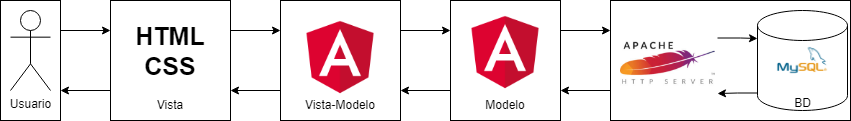
\includegraphics[scale=0.6]{arq-tec}}
\caption{Diagrama de la arquitectura tecnológica}
\end{figure}
%%\newpage
\chapter{PSI 7: DEFINICIÓN DE LA ARQUITECTURA TECNOLÓGICA}
	\vspace{2cm}	
	\begin{center}
	{\Large \textbf{FASE DE PLANIFICACIÓN} \par}
	\end{center}
	\vspace{5cm}
	
	\begin{center}
	\Huge \textbf{PSI}\par
	\end{center}

\newpage

\section{PSI 7.1: Identificación de las Necesidades de Infraestructura Tecnológica} 

\newpage
\section{PSI 7.2: Selección de la Arquitectura Tecnológica} 


\newpage
\chapter{ESTUDIO DE VIABILIDAD DEL SISTEMA}
	\vspace{2cm}	
	\begin{center}
	{\Large \textbf{FASE DE DESARROLLO} \par}
	\end{center}
	\vspace{5cm}
	
	\begin{center}
	\Huge \textbf{EVS}\par
	\end{center}\newpage
\section{EVS 4, 5, 6: ESTUDIO Y VALORACIÓN DE ALTERNATIVAS DE SOLUCIÓN. SELECCIÓN DE ALTERNATIVA FINAL}

\subsection{Evaluación de alternativas de desarrollo} 
\subsubsection{JavaScript y Node.js}
JavaScript es uno de los lenguajes más populares actualmente. Está basado en el estándar ECMAScript. Se trata un lenguaje interpretado, se compila en tiempo de ejecución. Es orientado a objetos, débilmente tipado y dinámico\cite{JavaScript}. 
\par Node.js es un entorno de ejecución de JavaScript orientado a eventos asíncronos, en el que no hace falta ultilizar hilos. Utiliza un modelo de entrada y salida sin bloqueo, lo que asegura un rendimiento más eficiente de la aplicación y evita que se produzca una gran sobrecarga del lado del servidor. Por ello, es muy apropiado para desarrollar sistemas escalables\cite{NodeJS}. Además, puede ser utilizado tanto en el lado del cliente como en el servidor, por lo que no se necesitaría una tecnología adicional para el back-end.
\par Esta fue la primera opción barajada, ya que había utilizado anteriormente estas tecnologías y podría aprovechar este proyecto para profundizar en su aprendizaje.
\begin{figure}[H]
	\centering
	\begin{subfigure}{0.3\textwidth}
	\centering
	
\includegraphics[scale=2.1]{javascript}
	\end{subfigure}
	\begin{subfigure}{0.3\textwidth}
	\centering
	
\includegraphics[scale=0.5]{nodejs}
	\end{subfigure}
	\caption{Logos de JavaScript y Node.js}
\end{figure}

\subsubsection{Angular, TypeScript y PHP}
La otra opción considerada fue Angular y TypeScript, debido a su popularidad. No había trabajado con ellas antes, y esta sería una buena oportunidad para conocerlas.
\par Angular es un framework desarrollado en TypeScript y utilizado habitualmente para crear aplicaciones de una sola página. Se basa en la utilización de componentes web reutilizables para crear aplicaciones web fácilmente escalables. Angular extiende la sintaxis de HTML y actualiza automáticamente el árbol DOM cuando el estado de un componente cambia. Cuenta con gran cantidad de librerías y es uno de los frameworks más utilizados en la industria actual\cite{Angular}.
\par TypeScript es un lenguaje de programación que extiende JavaScript añadiendo la definición de tipos estáticos. Al compilarlo se transforma en código JavaScript siguiendo todos los estándares, y puede ejecutarse en cualquier lugar que ejecute JavaScript\cite{TypeScript}.
\par En este caso, Angular y TypeScript son ambas tecnologías de front-end, por tanto necesitamos una tercera tecnología para el back-end de esta aplicación. Para ello consideré como opción PHP, lenguaje que se ejecuta en el servidor y envía el resultado generado al cliente, y que es otra de las tecnologías más reconocidas y usadas en el desarrollo web actualmente y desde su creación.
\begin{figure}[H]
	\centering
	\begin{subfigure}{0.2\textwidth}
	\centering
	
\includegraphics[scale=0.30]{angular}
	\end{subfigure}
	\begin{subfigure}{0.3\textwidth}
	\centering
	
\includegraphics[scale=0.12]{typescript}
	\end{subfigure}
	\begin{subfigure}{0.3\textwidth}
	\centering
	
\includegraphics[scale=0.05]{php}
	\end{subfigure}
	\caption {Logos de Angular, TypeScript y PHP}
\end{figure}
\noindent Ambas opciones son de código abierto, lo que me parece un punto positivo ya que, gracias a la colaboración de la comunidad, se consigue una alta calidad en el software. 
\par Finalmente, me decidí por Angular, TypeScript y PHP, principalmente por la razón de profundizar en el aprendizaje de estas tecnologías tan importantes actualmente en el desarrollo de aplicaciones web.

\subsection{Evaluación de alternativas de gestor de bases de datos} 
\subsubsection{MySQL}
MySQL es un SGBD relacional de código abierto con un modelo cliente-servidor. Ha sido la única opción considerada al tratarse de la base de datos relacional que es comúnmente utilizada con Angular, y no se ha encontrado ninguna necesidad o ventaja de usar un sistema no relacional.
\begin{figure}[H]
	\centering
	
\includegraphics[scale=0.1]{mysql}
	\caption{Logo de MySQL}
\end{figure}
\newpage
\chapter{PLANIFICACIÓN Y GESTIÓN DEL TFG}
\newpage

\newpage
\section{PLANIFICACIÓN DEL PROYECTO}

\subsection{Identificación de Interesados}
\begin{itemize}
\item \textbf{Usuarios de la aplicación web del museo}: Personas interesadas en la información ofrecida de las piezas expuestas en el museo que consultarán la página web.
\item \textbf{Tutor de este trabajo y administrador del museo}: Persona que ha propuesto el proyecto de digitalización del museo, y que lo administrará una vez terminado el desarrollo.
\item \textbf{Autora del trabajo y desarrolladora}: Encargada del desarrollo de la aplicación y de la documentación asociada.
\end{itemize}


\subsection{%OBS y 
PBS}
\begin{figure}[H]
\centering
\centerline{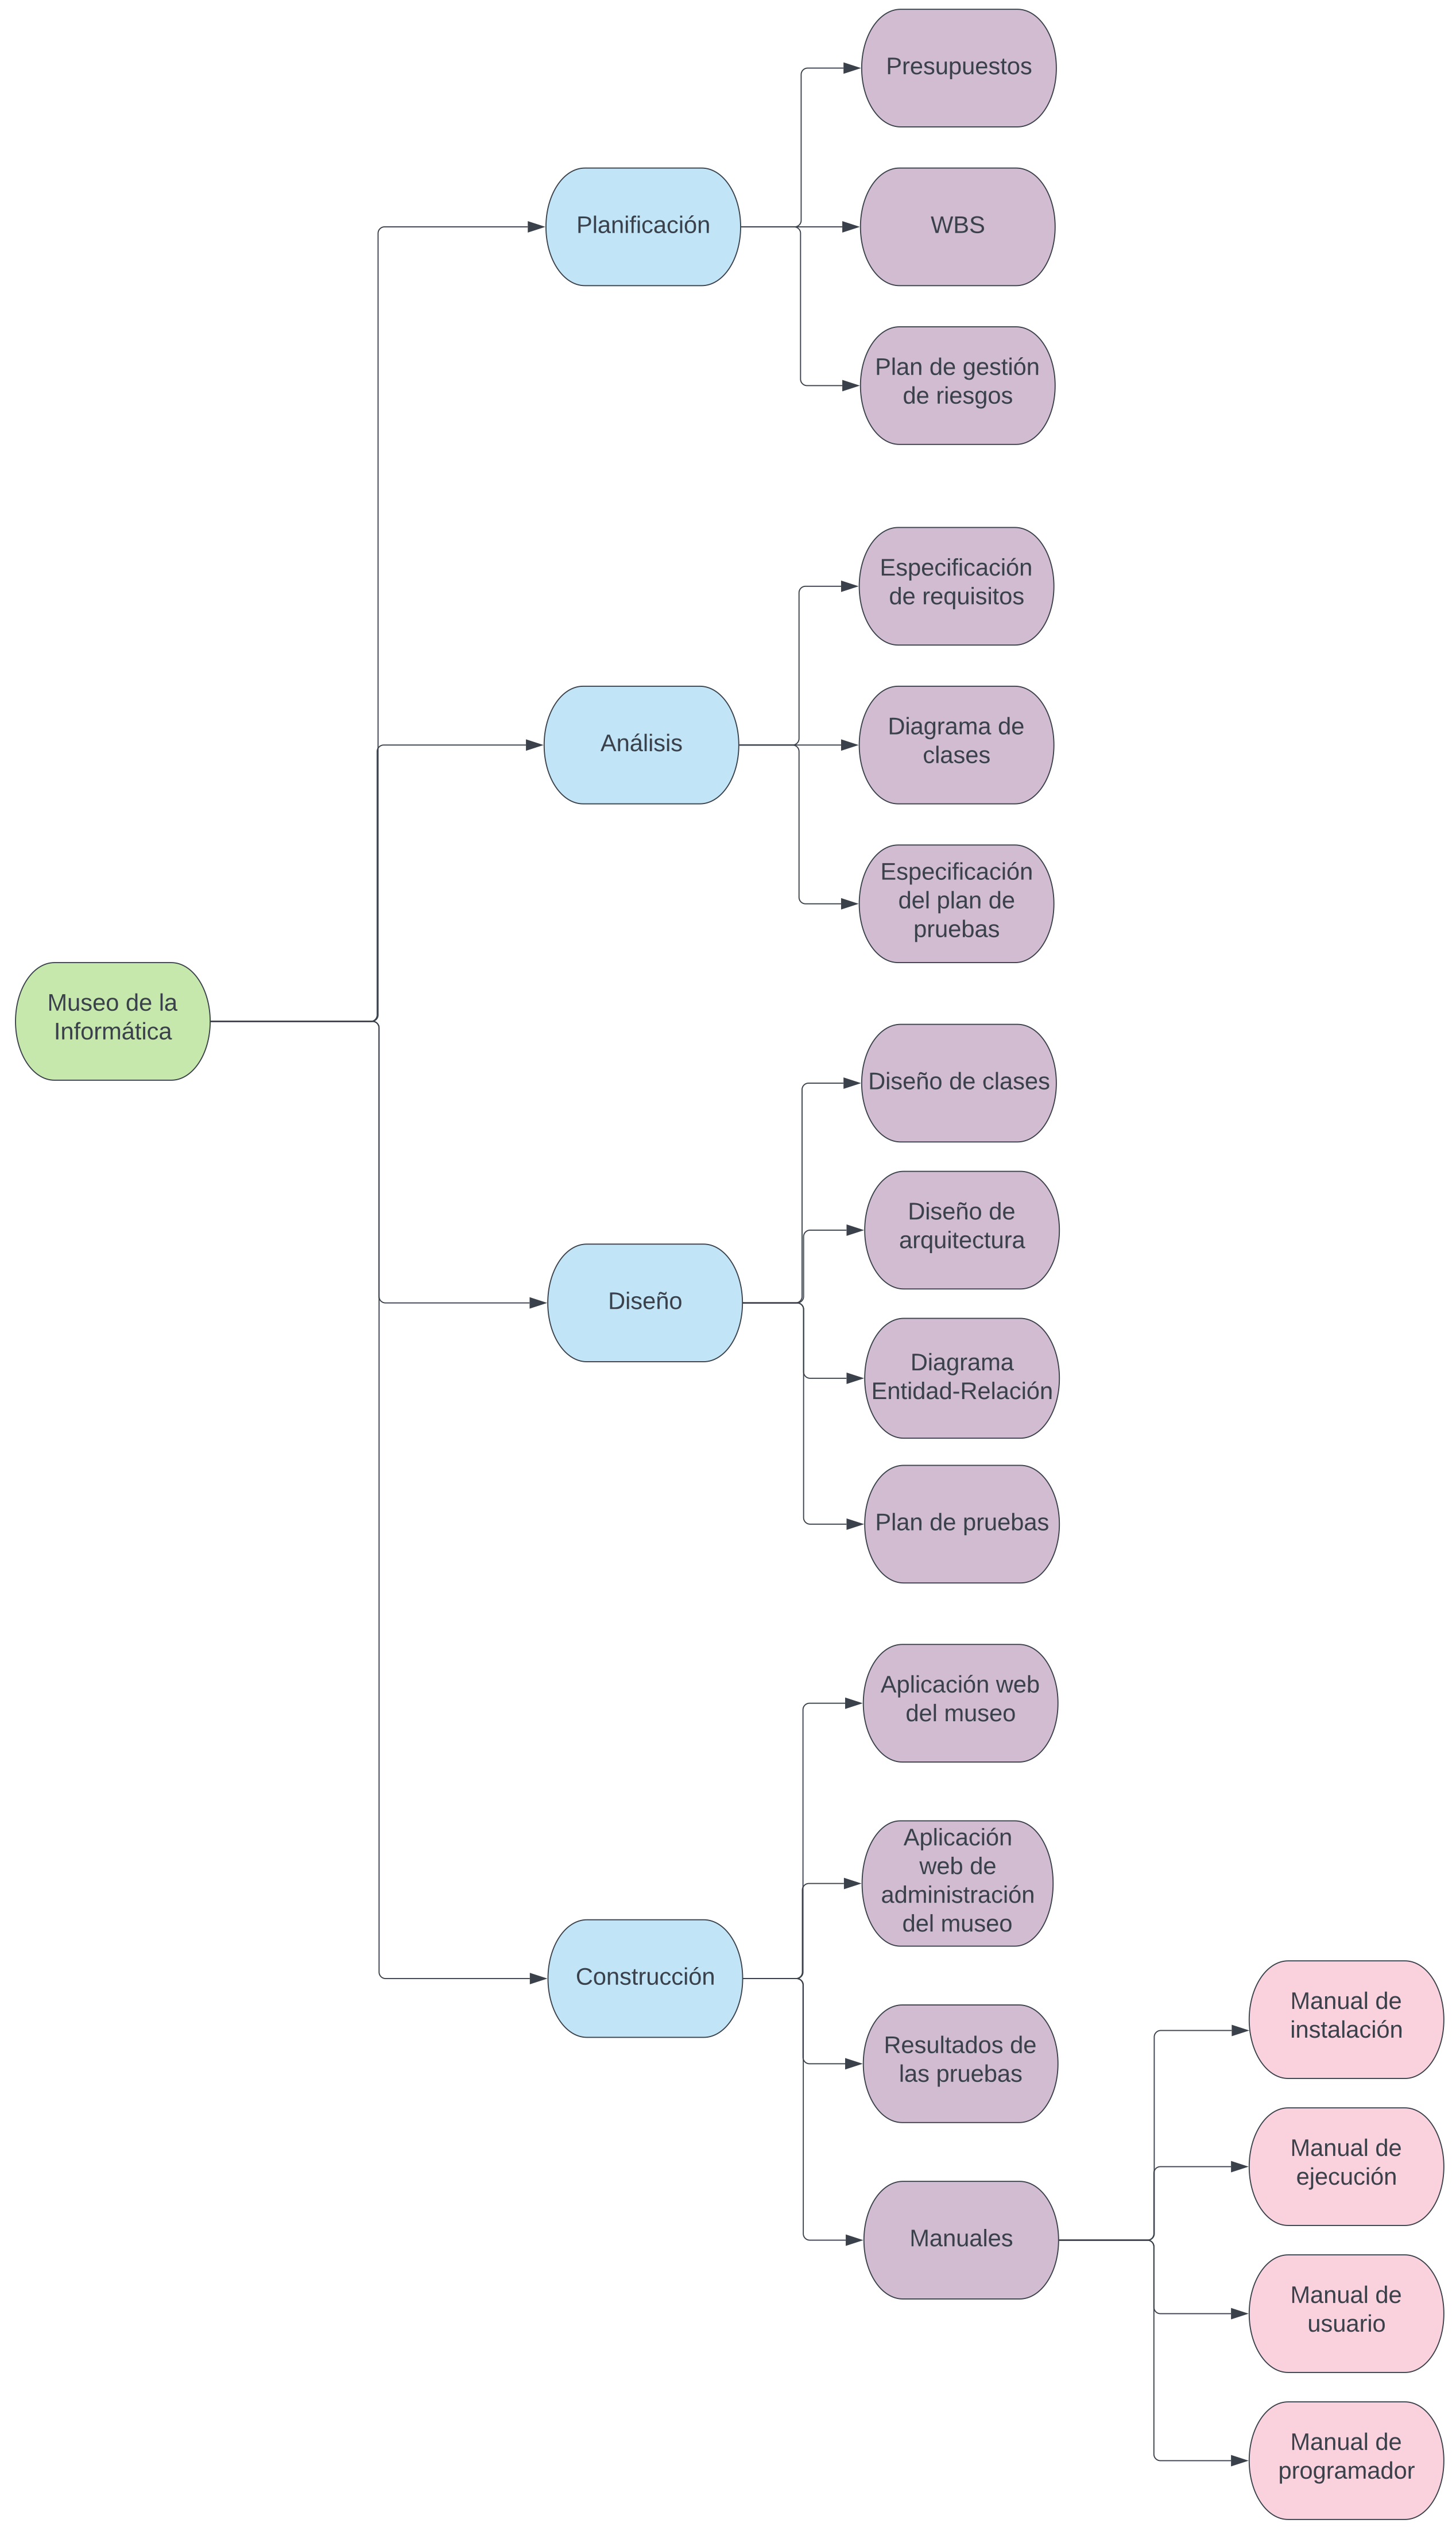
\includegraphics[scale=0.25]{PBS}}
\caption{Product Breakdown Structure}
\end{figure}


\subsection{Planificación Inicial. WBS}
A continuación se muestra la planificación inicial del proyecto y el correspondiente diagrama de Gantt. Para visualizar mejor esta planificación se adjunta el archivo \textit{WBS.mpp} como se especifica en la sección \ref{sec:contenido_anexos}. Se han planificado jornadas de trabajo de 3 horas diarias, y la estimación de la duración total del proyecto es de 258 horas.
\begin{landscape}
\pagestyle{empty}
\begin{figure}[H]
\centering
\centerline{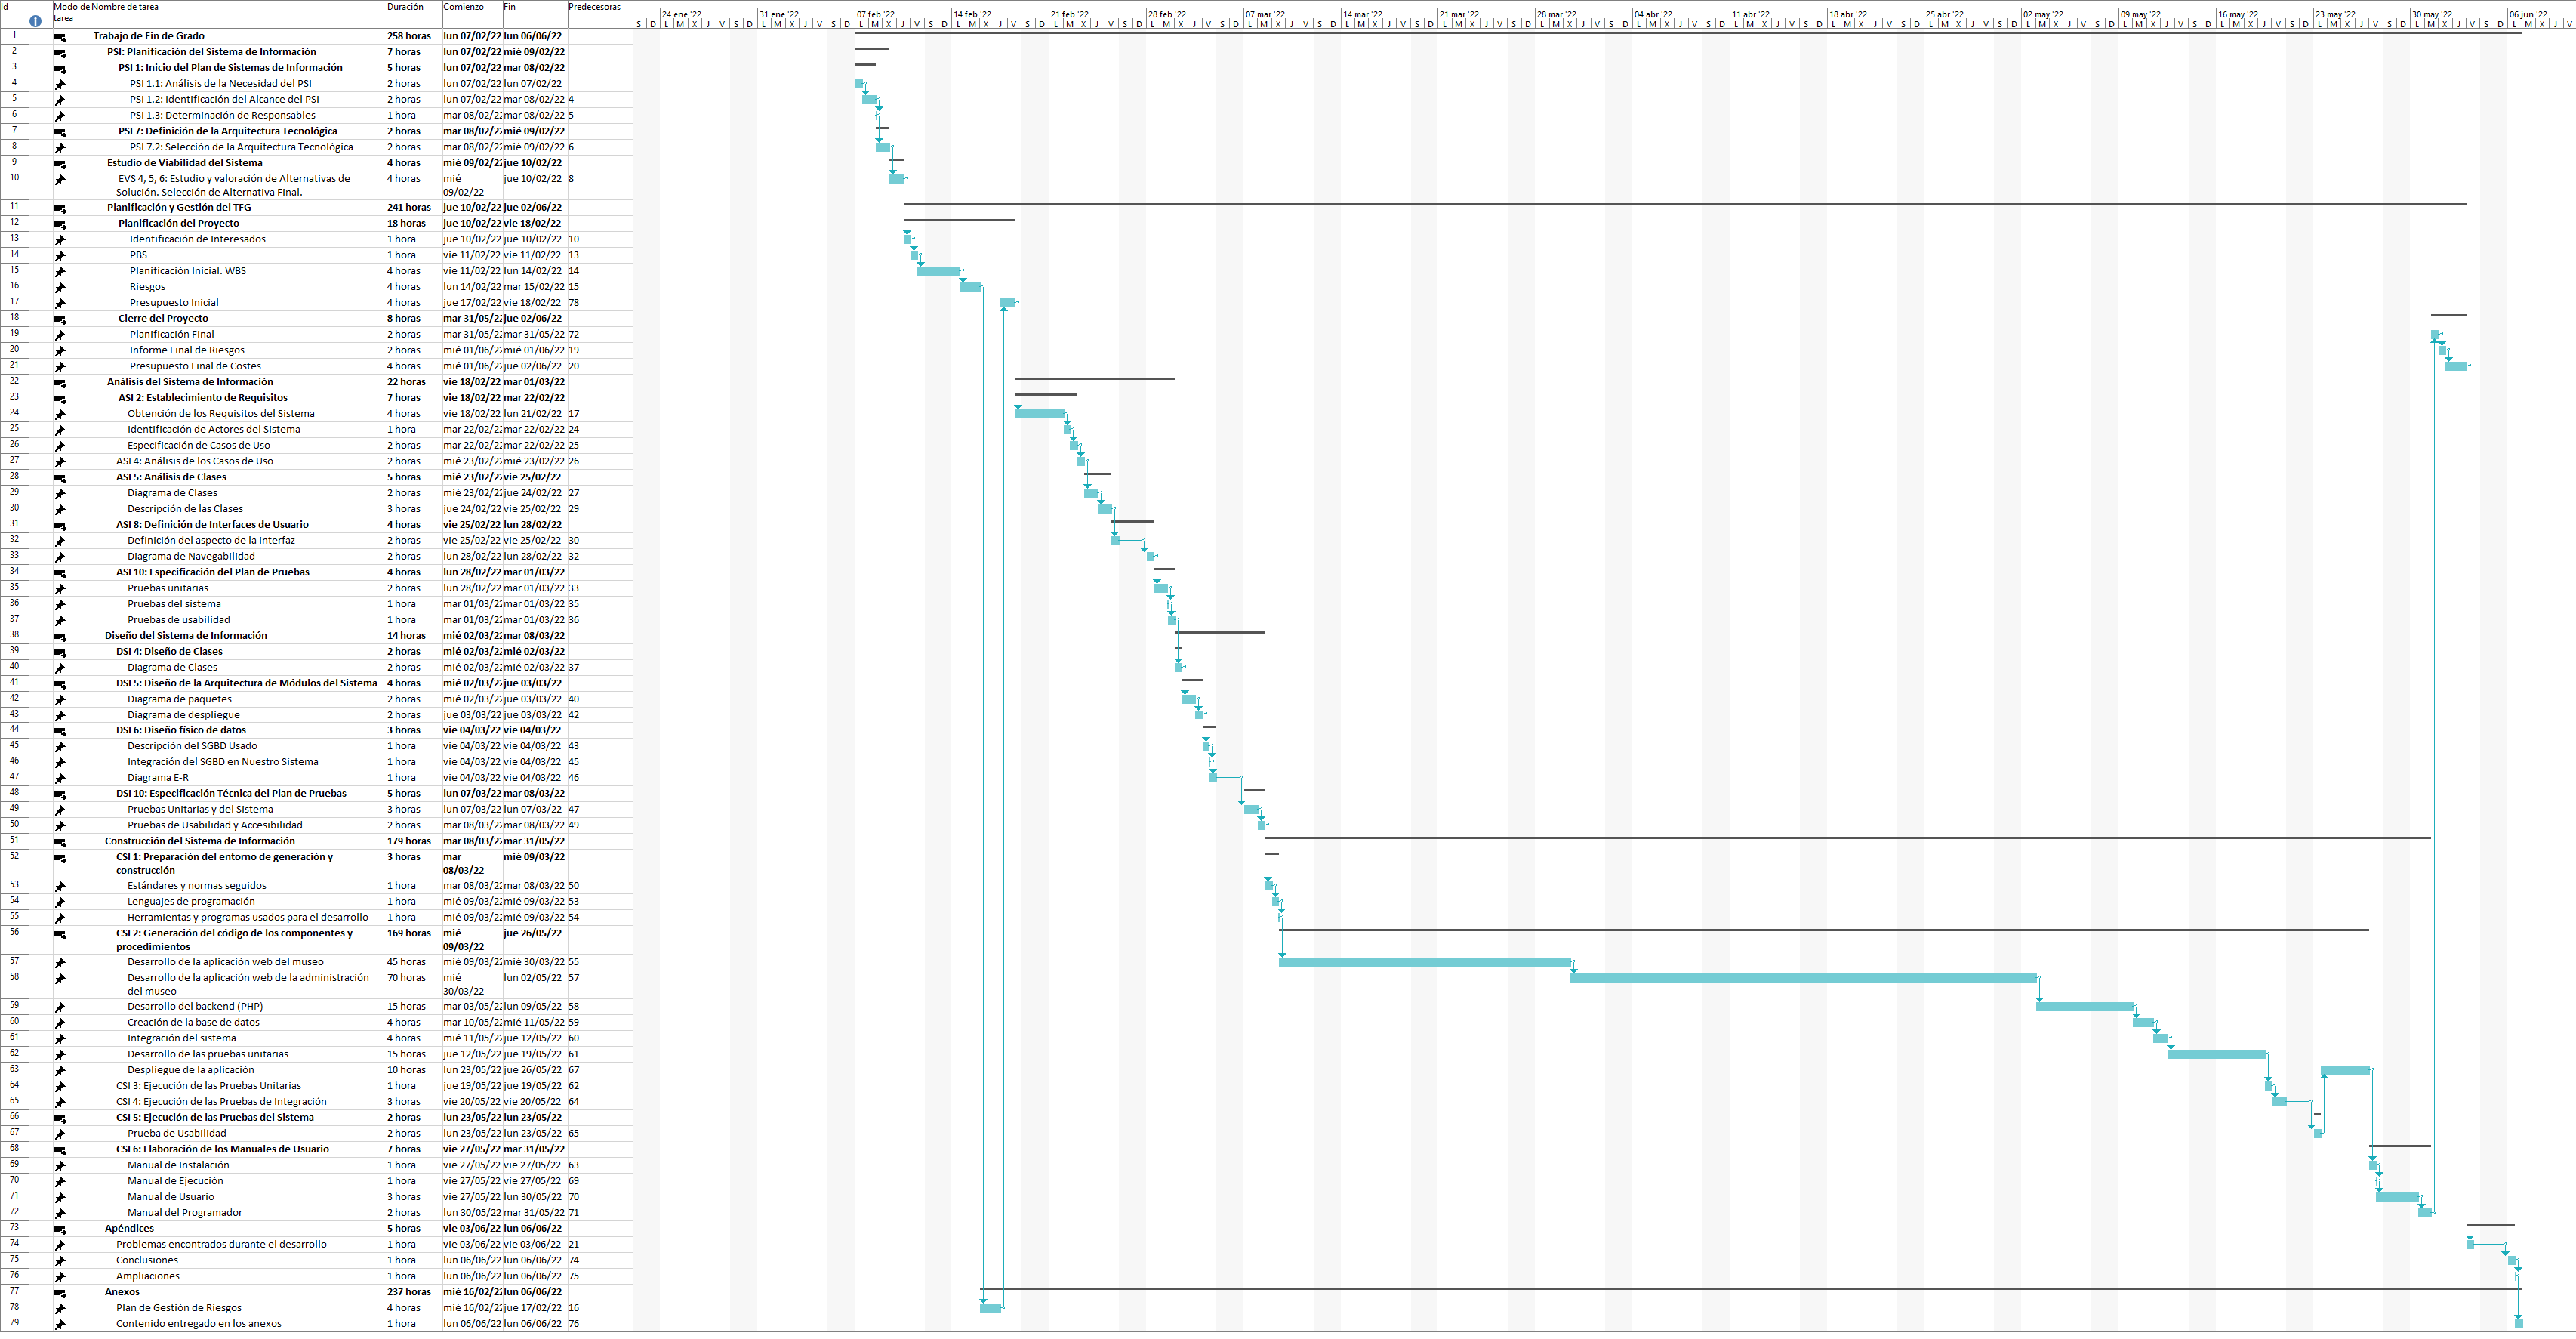
\includegraphics[scale=0.3]{plan-inicial}}
\caption{Planificación inicial, diagrama de Gantt}
\end{figure}

\end{landscape}
\pagestyle{fancy}
\subsection{Riesgos}

\subsubsection{Plan de Gestión de Riesgos} 

\subsubsection{Identificación de Riesgos}

\subsubsection{Registro de Riesgos} 



\subsection{Presupuesto Inicial}

\subsubsection{Presupuesto de Costes}

\subsubsection{Presupuesto de Cliente} 


%\newpage
%\section{EJECUCIÓN DEL PROYECTO}
%
%\subsection{Plan Seguimiento de Planificación}
%
%\subsection{Bitácora de Incidencias del Proyecto}
%
%\subsection{Riesgos}


\newpage
\section{CIERRE DEL PROYECTO}

\subsection{Planificación Final}

\subsection{Informe Final de Riesgos}

\subsection{Presupuesto Final de Costes}

\subsection{Informe de Lecciones Aprendidas}

\newpage
\chapter{ANÁLISIS DEL SISTEMA DE INFORMACIÓN}
	\vspace{2cm}	
	\begin{center}
	{\Large \textbf{FASE DE DESARROLLO} \par}
	\end{center}
	\vspace{5cm}
	
	\begin{center}
	\Huge \textbf{ASI}\par
	\end{center}

%\newpage
%\section{ASI 1: DEFINICIÓN DEL SISTEMA}

%\subsection{Determinación del Alcance del Sistema}



\newpage
\section{ASI 2: ESTABLECIMIENTO DE REQUISITOS}
\subsection{Obtención de los Requisitos del Sistema} 

\subsubsection{Requisitos de interfaces externas}

\paragraph*{Interfaces de usuario}
	
	\newlist{myEnumIU}{enumerate}{4}
	\setlist[myEnumIU,1]{label=\textbf{RIU-\arabic*.}}
	\setlist[myEnumIU,2]{label*=\textbf{\arabic*.}}
	\setlist[myEnumIU,3]{label*=\textbf{\arabic*.}}
	\setlist[myEnumIU,4]{label*=\textbf{\arabic*.}}

	\begin{myEnumIU}
		\item El sistema será accesible desde cualquier dispositivo que cuente con conexión a internet y un navegador web.
		\item El sistema estará disponible en diferentes idiomas.
		\begin{myEnumIU}
			\item Español
			\item Inglés
		\end{myEnumIU}
		\item El sistema deberá ser accesible para todos los usuarios a través de los navegadores más comunes.
		\begin{myEnumIU}
			\item Google Chrome
			\item Mozilla Firefox
			\item Microsoft Edge
		\end{myEnumIU}
		\item El usuario podrá utilizar todas las funcionalidades desarrolladas de la aplicación sin inconvenientes.
		\item El usuario no necesitará de conocimientos tecnológicos avanzados.
	\end{myEnumIU}

\paragraph*{Interfaces hardware}
	
	\newlist{myEnumIH}{enumerate}{4}
	\setlist[myEnumIH,1]{label=\textbf{RIH-\arabic*.}}
	\setlist[myEnumIH,2]{label*=\textbf{\arabic*.}}
	\setlist[myEnumIH,3]{label*=\textbf{\arabic*.}}
	\setlist[myEnumIH,4]{label*=\textbf{\arabic*.}}

	\begin{myEnumIH}
		\item El sistema dispondrá de una base de datos para almacenar la información necesaria.
	\end{myEnumIH}

%\paragraph*{Interfaces software}

\paragraph*{Interfaces de comunicaciones}

	\newlist{myEnumIC}{enumerate}{4}
	\setlist[myEnumIC,1]{label=\textbf{RIC-\arabic*.}}
	\setlist[myEnumIC,2]{label*=\textbf{\arabic*.}}
	\setlist[myEnumIC,3]{label*=\textbf{\arabic*.}}
	\setlist[myEnumIC,4]{label*=\textbf{\arabic*.}}

	\begin{myEnumIC}
		\item El sistema contendrá enlaces a diferentes sitios web.
		\item El sistema mostrará por defecto enlaces a los siguientes sitios web.
		\begin{myEnumIC}
			\item Twitter oficial de la Escuela de Ingeniería Informática
			\item Página web de la Escuela de Ingeniería Informática
			\item Página web de la Universidad de Oviedo
		\end{myEnumIC}
	\end{myEnumIC}



\subsubsection{Requisitos funcionales}

\newlist{myEnumerate}{enumerate}{9}
\setlist[myEnumerate,1]{label=\textbf{RF-\arabic*.}}
\setlist[myEnumerate,2]{label*=\textbf{\arabic*.}}
\setlist[myEnumerate,3]{label*=\textbf{\arabic*.}}
\setlist[myEnumerate,4]{label*=\textbf{\arabic*.}}
\setlist[myEnumerate,5]{label*=\textbf{\arabic*.}}
\setlist[myEnumerate,6]{label*=\textbf{\arabic*.}}
\setlist[myEnumerate,7]{label*=\textbf{\arabic*.}}
\setlist[myEnumerate,8]{label*=\textbf{\arabic*.}}
\setlist[myEnumerate,9]{label*=\textbf{\arabic*.}}

\begin{myEnumerate}
\item
\end{myEnumerate}


\subsubsection{Requisitos de rendimiento}
\subsubsection{Requisitos lógicos de BD}
\subsubsection{Requisitos de desarrollo}
\subsubsection{Restricciones de diseño}
\subsubsection{Atributos del sistema}


\subsection{Identificación de Actores del Sistema} 
\subsubsection{Usuario administrador}
Actor que interactúa con el sistema. Es responsable de gestionar el sistema y su mantenimiento. Es el único actor con acceso a la base de datos del sistema y capacidad de modificarla. Debe tener amplios conocimientos sobre el sistema.
\subsubsection{Usuario estándar}
Actor que interactúa con el sistema. Tiene acceso de lectura a toda la aplicación web, exceptuando la parte dedicada al mantenimiento. Solo debe tener un conocimiento básico para navegar por internet.

\subsection{Especificación de Casos de Uso}

\textcolor[rgb]{0.65,0.16,0}{Ejemplo de tabla para especificación de casos de uso}

\begin{table}[htbp]
  \centering
  \caption{Especificación Caso de Uso 1}
    \begin{tabular}{p{20.855em}r}
\cmidrule{1-1}    \rowcolor[rgb]{ .949,  .949,  .949} \multicolumn{1}{p{20.855em}}{\textbf{Nombre del caso de uso}} & \multicolumn{1}{r}{\cellcolor[rgb]{ 1,  1,  1}} \\
\cmidrule{1-1}    \multicolumn{1}{p{20.855em}}{Registro} & \multicolumn{1}{r}{} \\
    \midrule
    \rowcolor[rgb]{ .949,  .949,  .949} \multicolumn{2}{p{31.64em}}{\textbf{Descripción}} \\
    \midrule
    \multicolumn{2}{p{31.64em}}{Un usuario no registrado debe poder registrarse en el sistema mediante su cuenta de Google, lo que hará que automáticamente se inicie sesión en la aplicación.} \\
    \bottomrule
    \end{tabular}%
  \label{espec_caso_uso_1}%
  \vspace{-4mm}
\end{table}%



%\newpage
%\section{ASI 3: IDENTIFICACIÓN DE SUBSISTEMAS DE ANÁLISIS}
%
%\subsection{Descripción de los Subsistemas} 
%%A continuación se describen los subsistemas identificados en el análisis
%%\subsubsection{Vistas}
%%
%%\subsubsection{Modelos}
%%
%%\subsubsection{Bases de datos}
%%
%%\subsubsection{Servidor}
%
%
%\subsection{Descripción de los Interfaces entre Subsistemas}



\newpage
\section{ASI 4: ANÁLISIS DE LOS CASOS DE USO}
\subsection{Caso de Uso 1} 

\begin{table}[H]
  \centering
  \vspace{-5mm}
  \caption{Análisis del Caso de Uso 1}
    \begin{tabular}{p{7.5em}p{24.145em}}
    \toprule
    \rowcolor[rgb]{ .871,  .918,  .965} \multicolumn{2}{p{31.645em}}{\textbf{Consultar periodos (museo)}} \\
    \midrule
    \rowcolor[rgb]{ .906,  .902,  .902} \textbf{Precondiciones} & \cellcolor[rgb]{ 1,  1,  1}- \\
    \midrule
    \rowcolor[rgb]{ .906,  .902,  .902} \textbf{Postcondiciones} & \cellcolor[rgb]{ 1,  1,  1}- \\
    \midrule
    \rowcolor[rgb]{ .906,  .902,  .902} \textbf{Actores} & \cellcolor[rgb]{ 1,  1,  1}Usuario estándar \\
    \midrule
    \rowcolor[rgb]{ .906,  .902,  .902} \textbf{Descripción} & \cellcolor[rgb]{ 1,  1,  1}El usuario accederá a la vista principal del museo y podrá visualizar los periodos existentes. Podrá acceder a los periodos. Podrá acceder a los componentes de los periodos. Podrá realizar una búsqueda.\\
    \midrule
    \rowcolor[rgb]{ .906,  .902,  .902} \textbf{Escenarios          Secundarios} & \cellcolor[rgb]{ 1,  1,  1}  \\
    \bottomrule
    \end{tabular}%
\end{table}%
 
\subsection{Caso de Uso 2}
\begin{table}[H]
  \centering
  \vspace{-5mm}
  \caption{Análisis del Caso de Uso 2}
    \begin{tabular}{p{7.5em}p{24.145em}}
    \toprule
    \rowcolor[rgb]{ .871,  .918,  .965} \multicolumn{2}{p{31.645em}}{\textbf{Consultar componentes (museo)}} \\
    \midrule
    \rowcolor[rgb]{ .906,  .902,  .902} \textbf{Precondiciones} & \cellcolor[rgb]{ 1,  1,  1}- \\
    \midrule
    \rowcolor[rgb]{ .906,  .902,  .902} \textbf{Postcondiciones} & \cellcolor[rgb]{ 1,  1,  1}- \\
    \midrule
    \rowcolor[rgb]{ .906,  .902,  .902} \textbf{Actores} & \cellcolor[rgb]{ 1,  1,  1}Usuario estándar \\
    \midrule
    \rowcolor[rgb]{ .906,  .902,  .902} \textbf{Descripción} & \cellcolor[rgb]{ 1,  1,  1}El usuario accederá a la vista de un periodo y podrá visualizar los componentes pertenecientes al mismo. Podrá acceder a otros periodos. Podrá acceder a los otros componentes de ese periodo. \\
    \midrule
    \rowcolor[rgb]{ .906,  .902,  .902} \textbf{Escenarios          Secundarios} & \cellcolor[rgb]{ 1,  1,  1}  \\
    \bottomrule
    \end{tabular}%
\end{table}%
 
\subsection{Caso de Uso 3}
\begin{table}[H]
  \centering
  \vspace{-5mm}
  \caption{Análisis del Caso de Uso 3}
    \begin{tabular}{p{7.5em}p{24.145em}}
    \toprule
    \rowcolor[rgb]{ .871,  .918,  .965} \multicolumn{2}{p{31.645em}}{\textbf{Iniciar sesión}} \\
    \midrule
    \rowcolor[rgb]{ .906,  .902,  .902} \textbf{Precondiciones} & \cellcolor[rgb]{ 1,  1,  1}El usuario no debe haber iniciado sesión. \\
    \midrule
    \rowcolor[rgb]{ .906,  .902,  .902} \textbf{Postcondiciones} & \cellcolor[rgb]{ 1,  1,  1}- \\
    \midrule
    \rowcolor[rgb]{ .906,  .902,  .902} \textbf{Actores} & \cellcolor[rgb]{ 1,  1,  1}Usuario \\
    \midrule
    \rowcolor[rgb]{ .906,  .902,  .902} \textbf{Descripción} & \cellcolor[rgb]{ 1,  1,  1}El usuario accederá a la página principal de la aplicación de administración e introducirá su email y contraseña para iniciar sesión en el sistema. \\
    \midrule
    \rowcolor[rgb]{ .906,  .902,  .902} \textbf{Escenarios          Secundarios} & \cellcolor[rgb]{ 1,  1,  1} Los datos introducidos no se corresponden con los datos de un usuario con permiso de administrador. Se muestra un error y de nuevo se solicita iniciar sesión. \\
    \bottomrule
    \end{tabular}%
\end{table}%
 
\subsection{Caso de Uso 4}
\begin{table}[H]
  \centering
  \vspace{-5mm}
  \caption{Análisis del Caso de Uso 4}
    \begin{tabular}{p{7.5em}p{24.145em}}
    \toprule
    \rowcolor[rgb]{ .871,  .918,  .965} \multicolumn{2}{p{31.645em}}{\textbf{Consultar periodos (administración)}} \\
    \midrule
    \rowcolor[rgb]{ .906,  .902,  .902} \textbf{Precondiciones} & \cellcolor[rgb]{ 1,  1,  1}El usuario debe haber iniciado sesión. \\
    \midrule
    \rowcolor[rgb]{ .906,  .902,  .902} \textbf{Postcondiciones} & \cellcolor[rgb]{ 1,  1,  1}- \\
    \midrule
    \rowcolor[rgb]{ .906,  .902,  .902} \textbf{Actores} & \cellcolor[rgb]{ 1,  1,  1}Usuario administrador \\
    \midrule
    \rowcolor[rgb]{ .906,  .902,  .902} \textbf{Descripción} & \cellcolor[rgb]{ 1,  1,  1}El usuario accederá al listado de periodos. Podrá acceder a cada uno de ellos. \\
    \midrule
    \rowcolor[rgb]{ .906,  .902,  .902} \textbf{Escenarios          Secundarios} & \cellcolor[rgb]{ 1,  1,  1}Aún no existe ningún periodo en el sistema. Se muestra una tabla vacía. \\
    \bottomrule
    \end{tabular}%
\end{table}
 
\subsection{Caso de Uso 5}
\begin{table}[H]
  \centering
  \vspace{-5mm}
  \caption{Análisis del Caso de Uso 5}
    \begin{tabular}{p{7.5em}p{24.145em}}
    \toprule
    \rowcolor[rgb]{ .871,  .918,  .965} \multicolumn{2}{p{31.645em}}{\textbf{Añadir periodo}} \\
    \midrule
    \rowcolor[rgb]{ .906,  .902,  .902} \textbf{Precondiciones} & \cellcolor[rgb]{ 1,  1,  1}El usuario debe haber iniciado sesión. \\
    \midrule
    \rowcolor[rgb]{ .906,  .902,  .902} \textbf{Postcondiciones} & \cellcolor[rgb]{ 1,  1,  1}El periodo añadido se guardará en la base de datos. \\
    \midrule
    \rowcolor[rgb]{ .906,  .902,  .902} \textbf{Actores} & \cellcolor[rgb]{ 1,  1,  1}Usuario administrador \\
    \midrule
    \rowcolor[rgb]{ .906,  .902,  .902} \textbf{Descripción} & \cellcolor[rgb]{ 1,  1,  1}El usuario accede al formulario para añadir un periodo. Rellena los campos necesarios. Pulsa el botón de guardar. \\
    \midrule
    \rowcolor[rgb]{ .906,  .902,  .902} \textbf{Escenarios          Secundarios} & \cellcolor[rgb]{ 1,  1,  1}- Se pulsa el botón cancelar. El formulario se restablece.\par - Se intenta acceder a otra página de la aplicación sin haber guardado los cambios. Se avisa de la situación y se pide una confirmación para continuar.\par - No se puede añadir el periodo. Se mostrará un error avisando de la situación. \\
    \bottomrule
    \end{tabular}%
\end{table}%
 
\subsection{Caso de Uso 6}
\begin{table}[H]
  \centering
  \vspace{-5mm}
  \caption{Análisis del Caso de Uso 6}
    \begin{tabular}{p{7.5em}p{24.145em}}
    \toprule
    \rowcolor[rgb]{ .871,  .918,  .965} \multicolumn{2}{p{31.645em}}{\textbf{Modificar periodo}} \\
    \midrule
    \rowcolor[rgb]{ .906,  .902,  .902} \textbf{Precondiciones} & \cellcolor[rgb]{ 1,  1,  1}El usuario debe haber iniciado sesión. Debe existir al menos un periodo. \\
    \midrule
    \rowcolor[rgb]{ .906,  .902,  .902} \textbf{Postcondiciones} & \cellcolor[rgb]{ 1,  1,  1}Los cambios realizados al periodo se guardarán en la base de datos. \\
    \midrule
    \rowcolor[rgb]{ .906,  .902,  .902} \textbf{Actores} & \cellcolor[rgb]{ 1,  1,  1}Usuario administrador \\
    \midrule
    \rowcolor[rgb]{ .906,  .902,  .902} \textbf{Descripción} & \cellcolor[rgb]{ 1,  1,  1}El usuario accede al periodo deseado y selecciona la opción de editar. Se mostrará el formulario correspondiente. Se realizan los cambios en el formulario. Pulsa el botón de guardar. \\
    \midrule
    \rowcolor[rgb]{ .906,  .902,  .902} \textbf{Escenarios          Secundarios} & \cellcolor[rgb]{ 1,  1,  1}- Se pulsa el botón cancelar. El formulario se restablece.\par - Se intenta acceder a otra página de la aplicación sin haber guardado los cambios. Se avisa de la situación y se pide una confirmación para continuar.\par - No se puede modificar el periodo. Se mostrará un error avisando de la situación. \\
    \bottomrule
    \end{tabular}%
\end{table}%
 
\subsection{Caso de Uso 7}
\begin{table}[H]
  \centering
  \vspace{-5mm}
  \caption{Análisis del Caso de Uso 7}
    \begin{tabular}{p{7.5em}p{24.145em}}
    \toprule
    \rowcolor[rgb]{ .871,  .918,  .965} \multicolumn{2}{p{31.645em}}{\textbf{Eliminar periodo}} \\
    \midrule
    \rowcolor[rgb]{ .906,  .902,  .902} \textbf{Precondiciones} & \cellcolor[rgb]{ 1,  1,  1}El usuario debe haber iniciado sesión. Debe existir al menos un periodo. \\
    \midrule
    \rowcolor[rgb]{ .906,  .902,  .902} \textbf{Postcondiciones} & \cellcolor[rgb]{ 1,  1,  1}El periodo eliminado y los componentes que pertenecen al mismo se borrarán de la base de datos y dejarán de mostrarse en la aplicación. \\
    \midrule
    \rowcolor[rgb]{ .906,  .902,  .902} \textbf{Actores} & \cellcolor[rgb]{ 1,  1,  1}Usuario administrador \\
    \midrule
    \rowcolor[rgb]{ .906,  .902,  .902} \textbf{Descripción} & \cellcolor[rgb]{ 1,  1,  1}El usuario accede al periodo deseado y selecciona la opción de eliminar. Se pide confirmación para eliminarlo. Se acepta esta confirmación. \\
    \midrule
    \rowcolor[rgb]{ .906,  .902,  .902} \textbf{Escenarios          Secundarios} & \cellcolor[rgb]{ 1,  1,  1}- No se acepta la confirmación para eliminarlo. El periodo y sus componentes permanecen en la base de datos.\par - No se puede eliminar el periodo. Se mostrará un error avisando de la situación. \\
    \bottomrule
    \end{tabular}%
\end{table}%
 
\subsection{Caso de Uso 8}
\begin{table}[H]
  \centering
  \vspace{-5mm}
  \caption{Análisis del Caso de Uso 8}
    \begin{tabular}{p{7.5em}p{24.145em}}
    \toprule
    \rowcolor[rgb]{ .871,  .918,  .965} \multicolumn{2}{p{31.645em}}{\textbf{Consultar componentes (administración)}} \\
    \midrule
    \rowcolor[rgb]{ .906,  .902,  .902} \textbf{Precondiciones} & \cellcolor[rgb]{ 1,  1,  1}El usuario debe haber iniciado sesión. Debe existir al menos un periodo. \\
    \midrule
    \rowcolor[rgb]{ .906,  .902,  .902} \textbf{Postcondiciones} & \cellcolor[rgb]{ 1,  1,  1}- \\
    \midrule
    \rowcolor[rgb]{ .906,  .902,  .902} \textbf{Actores} & \cellcolor[rgb]{ 1,  1,  1}Usuario administrador \\
    \midrule
    \rowcolor[rgb]{ .906,  .902,  .902} \textbf{Descripción} & \cellcolor[rgb]{ 1,  1,  1}El usuario accederá a un periodo existente y visualizará los componentes pertenecientes a este. Podrá acceder a cada uno de ellos. \\
    \midrule
    \rowcolor[rgb]{ .906,  .902,  .902} \textbf{Escenarios          Secundarios} & \cellcolor[rgb]{ 1,  1,  1}Aún no existen componentes para el periodo que se consulta. Se mostrará una tabla vacía. \\
    \bottomrule
    \end{tabular}%
\end{table}%
 
\subsection{Caso de Uso 9}
\begin{table}[H]
  \centering
  \vspace{-5mm}
  \caption{Análisis del Caso de Uso 9}
    \begin{tabular}{p{7.5em}p{24.145em}}
    \toprule
    \rowcolor[rgb]{ .871,  .918,  .965} \multicolumn{2}{p{31.645em}}{\textbf{Añadir componente}} \\
    \midrule
    \rowcolor[rgb]{ .906,  .902,  .902} \textbf{Precondiciones} & \cellcolor[rgb]{ 1,  1,  1}El usuario debe haber iniciado sesión. Debe existir al menos un periodo. \\
    \midrule
    \rowcolor[rgb]{ .906,  .902,  .902} \textbf{Postcondiciones} & \cellcolor[rgb]{ 1,  1,  1}El componente añadido se guardará en la base de datos y se asociará al periodo correspondiente. \\
    \midrule
    \rowcolor[rgb]{ .906,  .902,  .902} \textbf{Actores} & \cellcolor[rgb]{ 1,  1,  1}Usuario administrador \\
    \midrule
    \rowcolor[rgb]{ .906,  .902,  .902} \textbf{Descripción} & \cellcolor[rgb]{ 1,  1,  1}El usuario accede al formulario para añadir un componente. Rellena los campos necesarios. Pulsa el botón de guardar. \\
    \midrule
    \rowcolor[rgb]{ .906,  .902,  .902} \textbf{Escenarios          Secundarios} & \cellcolor[rgb]{ 1,  1,  1}- Se pulsa el botón cancelar. El formulario se restablece.\par - Se intenta acceder a otra página de la aplicación sin haber guardado los cambios. Se avisa de la situación y se pide una confirmación para continuar.\par - No se puede añadir el componente. Se mostrará un error avisando de la situación.  \\
    \bottomrule
    \end{tabular}%
\end{table}%
 
\subsection{Caso de Uso 10}
\begin{table}[H]
  \centering
  \vspace{-5mm}
  \caption{Análisis del Caso de Uso 10}
    \begin{tabular}{p{7.5em}p{24.145em}}
    \toprule
    \rowcolor[rgb]{ .871,  .918,  .965} \multicolumn{2}{p{31.645em}}{\textbf{Modificar componente}} \\
    \midrule
    \rowcolor[rgb]{ .906,  .902,  .902} \textbf{Precondiciones} & \cellcolor[rgb]{ 1,  1,  1}El usuario debe haber iniciado sesión. Debe existir al menos un componente. \\
    \midrule
    \rowcolor[rgb]{ .906,  .902,  .902} \textbf{Postcondiciones} & \cellcolor[rgb]{ 1,  1,  1}Los cambios realizados en el componente se guardarán en la base de datos. \\
    \midrule
    \rowcolor[rgb]{ .906,  .902,  .902} \textbf{Actores} & \cellcolor[rgb]{ 1,  1,  1}Usuario administrador \\
    \midrule
    \rowcolor[rgb]{ .906,  .902,  .902} \textbf{Descripción} & \cellcolor[rgb]{ 1,  1,  1}El usuario accede al componente deseado y selecciona la opción de editar. Se mostrará el formulario correspondiente. Se realizan los cambios en el formulario. Pulsa el botón de guardar. \\
    \midrule
    \rowcolor[rgb]{ .906,  .902,  .902} \textbf{Escenarios          Secundarios} & \cellcolor[rgb]{ 1,  1,  1}- Se pulsa el botón cancelar. El formulario se restablece.\par - Se intenta acceder a otra página de la aplicación sin haber guardado los cambios. Se avisa de la situación y se pide una confirmación para continuar.\par - No se puede modificar el componente. Se mostrará un error avisando de la situación.  \\
    \bottomrule
    \end{tabular}%
\end{table}
 
\subsection{Caso de Uso 11}
\begin{table}[H]
  \centering
  \vspace{-5mm}
  \caption{Análisis del Caso de Uso 11}
    \begin{tabular}{p{7.5em}p{24.145em}}
    \toprule
    \rowcolor[rgb]{ .871,  .918,  .965} \multicolumn{2}{p{31.645em}}{\textbf{Eliminar componente}} \\
    \midrule
    \rowcolor[rgb]{ .906,  .902,  .902} \textbf{Precondiciones} & \cellcolor[rgb]{ 1,  1,  1}El usuario debe haber iniciado sesión. Debe existir al menos un componente. \\
    \midrule
    \rowcolor[rgb]{ .906,  .902,  .902} \textbf{Postcondiciones} & \cellcolor[rgb]{ 1,  1,  1}El componente eliminado  se borrará de la base de datos y dejará de mostrarse en la aplicación. \\
    \midrule
    \rowcolor[rgb]{ .906,  .902,  .902} \textbf{Actores} & \cellcolor[rgb]{ 1,  1,  1}Usuario administrador \\
    \midrule
    \rowcolor[rgb]{ .906,  .902,  .902} \textbf{Descripción} & \cellcolor[rgb]{ 1,  1,  1}El usuario accede al componente deseado y selecciona la opción de eliminar. Se pide confirmación para eliminarlo. Se acepta esta confirmación.  \\
    \midrule
    \rowcolor[rgb]{ .906,  .902,  .902} \textbf{Escenarios          Secundarios} & \cellcolor[rgb]{ 1,  1,  1}- No se acepta la confirmación para eliminarlo. El componente permanece en la base de datos.\par - No se puede eliminar el componente. Se mostrará un error avisando de la situación.  \\
    \bottomrule
    \end{tabular}%
\end{table}%


\newpage
\section{ASI 5: ANÁLISIS DE CLASES}

\subsection{Diagrama de Clases} 
\subsubsection{Museo}
\begin{figure}[H]
\centering
\centerline{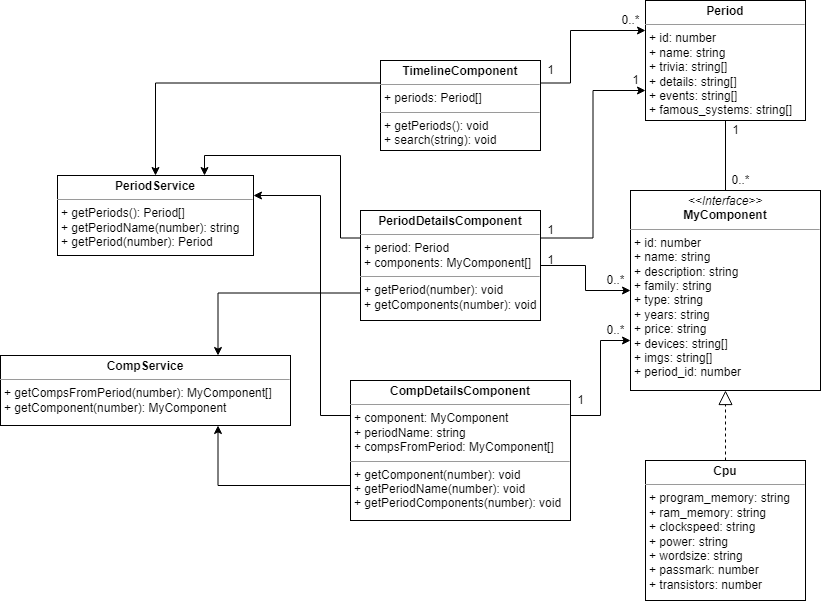
\includegraphics[scale=0.5]{asi-clases-museo}}
\caption{Análisis de clases: diagrama de clases del museo}
\end{figure}
\subsubsection{Administración del museo}
\begin{figure}[H]
\centering
\centerline{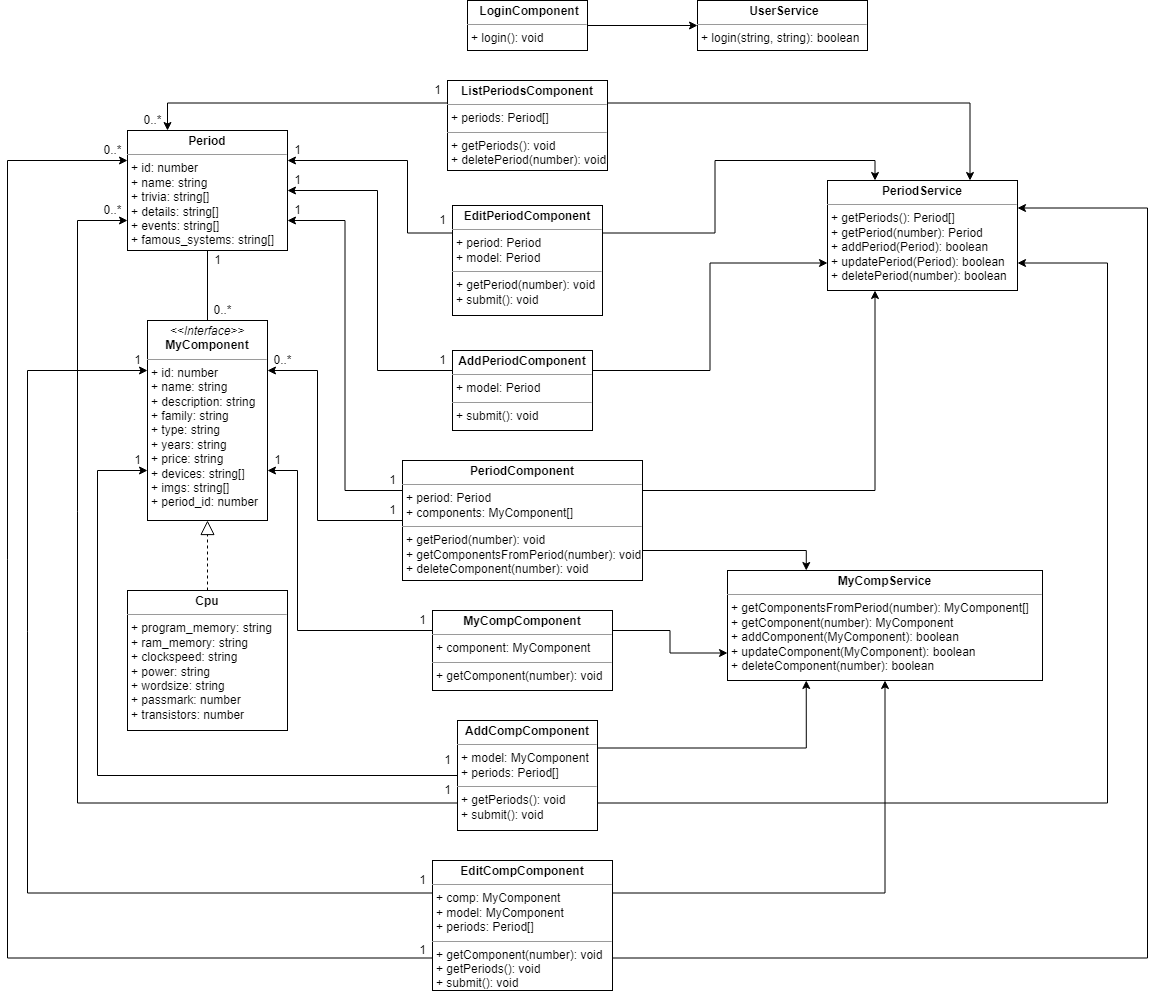
\includegraphics[scale=0.5]{asi-clases-admin}}
\caption{Análisis de clases: diagrama de clases de la administración}
\end{figure}

\subsection{Descripción de las Clases}
\textit{Period}, \textit{MyComponent} y \textit{Cpu} son iguales en el proyecto del museo y en el de la administración, por lo tanto se describen una única vez a continuación:

\begin{table}[H]
\vspace{-4mm}
  \centering
  \caption{Descripción de la clase Period}
    \begin{tabular}{p{8.645em}p{5em}p{15.5em}}
    \toprule
    \rowcolor[rgb]{ .851,  .886,  .953} \multicolumn{3}{p{31.285em}}{\textbf{Periodo}} \\ \midrule
    \rowcolor[rgb]{ .949,  .949,  .949} \multicolumn{3}{p{31.285em}}{\textbf{Descripción}} \\ \midrule
    \multicolumn{3}{p{31.285em}}{Clase que modela un periodo.} \\ \midrule
    \rowcolor[rgb]{ .906,  .902,  .902} \multicolumn{3}{p{31.285em}}{\textbf{Atributos propuestos}} \\ \midrule
    \textbf{id} & number & Identificador del periodo\\
    \textbf{name} & string & Nombre del periodo \\ 
    \textbf{trivia} & string[] & Curiosidades del periodo \\
    \textbf{details} & string[] & Detalles del periodo \\
    \textbf{events} & string[] & Eventos ocurridos durante este periodo \\
    \textbf{famous\_systems} & string[] & Sistemas famosos que llevaban componentes pertenecientes al periodo \\ \midrule
    \rowcolor[rgb]{ .906,  .902,  .902} \multicolumn{3}{p{31.285em}}{\textbf{Métodos propuestos}} \\ \midrule
    \multicolumn{3}{p{31.285em}}{-} \\ \bottomrule
    \end{tabular}%
\end{table}%

\begin{table}[H]
\vspace{-4mm}
  \centering
  \caption{Descripción de la interfaz MyComponent }
    \begin{tabular}{p{8.645em}p{5em}p{15.5em}}
    \toprule
    \rowcolor[rgb]{ .851,  .886,  .953} \multicolumn{3}{p{31.285em}}{\textbf{MyComponent}} \\ \midrule
    \rowcolor[rgb]{ .949,  .949,  .949} \multicolumn{3}{p{31.285em}}{\textbf{Descripción}} \\ \midrule
    \multicolumn{3}{p{31.285em}}{Interfaz que modela los atributos genéricos de un componente.} \\ \midrule
    \rowcolor[rgb]{ .906,  .902,  .902} \multicolumn{3}{p{31.285em}}{\textbf{Atributos propuestos}} \\ \midrule
    \textbf{id} & number & Identificador del componente\\
    \textbf{name} & string & Nombre del componente \\ 
    \textbf{description} & string & Descripción del componente \\
    \textbf{family} & string & Familia a la que pertenece \\
    \textbf{type} & string & Tipo de componente (CPU, genérico...) \\
    \textbf{years} & string & Rango de años en los que se utilizó \\
    \textbf{price} & string & Precio de venta del componente \\
    \textbf{devices} & string[] & Tipo de dispositivos en los que se usaba el componente (portátiles o de escritorio) \\
    \textbf{imgs} & string[] & Nombres de las imágenes del componente \\
    \textbf{period\_id} & number & Identificador del periodo al que pertenece el componente \\ \midrule
    \rowcolor[rgb]{ .906,  .902,  .902} \multicolumn{3}{p{31.285em}}{\textbf{Métodos propuestos}} \\ \midrule
    \multicolumn{3}{p{31.285em}}{-} \\ \bottomrule
    \end{tabular}%
\end{table}%

\begin{table}[H]
\vspace{-4mm}
  \centering
  \caption{Descripción de la clase Cpu}
    \begin{tabular}{p{8.645em}p{5em}p{15.5em}}
    \toprule
    \rowcolor[rgb]{ .851,  .886,  .953} \multicolumn{3}{p{31.285em}}{\textbf{Cpu}} \\ \midrule
    \rowcolor[rgb]{ .949,  .949,  .949} \multicolumn{3}{p{31.285em}}{\textbf{Descripción}} \\ \midrule
    \multicolumn{3}{p{31.285em}}{Clase que implementa la interfaz MyComponent. Modela una CPU, con sus atributos específicos correspondientes. } \\ \midrule
    \rowcolor[rgb]{ .906,  .902,  .902} \multicolumn{3}{p{31.285em}}{\textbf{Atributos propuestos}} \\ \midrule
    \textbf{program\_memory} & string & Memoria ROM de la CPU\\
    \textbf{ram\_memory} & string & Memoria RAM de la CPU\\
    \textbf{clockspeed} & string & Velocidad de reloj de la CPU\\ 
    \textbf{power} & string & Potencia de la CPU\\
    \textbf{wordsize} & string & Tamaño de palabra de la CPU\\
    \textbf{passmark} & number & Passmark de la CPU\\
    \textbf{transistors} & number & Número de transistores de la CPU\\ \midrule
    \rowcolor[rgb]{ .906,  .902,  .902} \multicolumn{3}{p{31.285em}}{\textbf{Métodos propuestos}} \\ \midrule
    \multicolumn{3}{p{31.285em}}{-} \\ \bottomrule
    \end{tabular}%
\end{table}%

\subsubsection{Museo}

\begin{table}[H]
\vspace{-4mm}
  \centering
  \caption{Descripción de la clase PeriodService (museo)}
    \begin{tabular}{p{8.645em}p{5em}p{15.5em}}
    \toprule
    \rowcolor[rgb]{ .851,  .886,  .953} \multicolumn{3}{p{31.285em}}{\textbf{PeriodService}} \\ \midrule
    \rowcolor[rgb]{ .949,  .949,  .949} \multicolumn{3}{p{31.285em}}{\textbf{Descripción}} \\ \midrule
    \multicolumn{3}{p{31.285em}}{Servicio que conecta con el back-end de la aplicación para realizar las operaciones relacionadas con los periodos.} \\ \midrule
    \rowcolor[rgb]{ .906,  .902,  .902} \multicolumn{3}{p{31.285em}}{\textbf{Atributos propuestos}} \\ \midrule
    \multicolumn{3}{p{31.285em}}{-} \\ \midrule
    \rowcolor[rgb]{ .906,  .902,  .902} \multicolumn{3}{p{31.285em}}{\textbf{Métodos propuestos}} \\ \midrule
    \textbf{getPeriods} & \multicolumn{2}{p{22.64em}}{Devuelve todos los periodos existentes.} \\ 
    \textbf{getPeriodName} & \multicolumn{2}{p{22.64em}}{Devuelve el nombre del periodo correspondiente al identificador pasado por parámetro.} \\ 
    \textbf{getPeriod} & \multicolumn{2}{p{22.64em}}{Devuelve el periodo cuyo identificador se pasa como parámetro.} \\ \bottomrule
    \end{tabular}%
\end{table}%

\begin{table}[H]
\vspace{-4mm}
  \centering
  \caption{Descripción de la clase CompService (museo)}
    \begin{tabular}{p{10em}p{5em}p{14.5em}}
    \toprule
    \rowcolor[rgb]{ .851,  .886,  .953} \multicolumn{3}{p{31.285em}}{\textbf{CompService}} \\ \midrule
    \rowcolor[rgb]{ .949,  .949,  .949} \multicolumn{3}{p{31.285em}}{\textbf{Descripción}} \\ \midrule
    \multicolumn{3}{p{31.285em}}{Servicio que conecta con el back-end de la aplicación para realizar las operaciones relacionadas con los componentes.} \\ \midrule
    \rowcolor[rgb]{ .906,  .902,  .902} \multicolumn{3}{p{31.285em}}{\textbf{Atributos propuestos}} \\ \midrule
    \multicolumn{3}{p{31.285em}}{-} \\ \midrule
    \rowcolor[rgb]{ .906,  .902,  .902} \multicolumn{3}{p{31.285em}}{\textbf{Métodos propuestos}} \\ \midrule
    \textbf{getCompsFromPeriod} & \multicolumn{2}{p{19.64em}}{Devuelve los componentes pertenecientes al periodo cuyo identificador se pasa como parámetro.} \\ 
    \textbf{getComponent} & \multicolumn{2}{p{19.64em}}{Devuelve el componente cuyo identificador se pasa como parámetro.} \\ \bottomrule
    \end{tabular}%
\end{table}%

\begin{table}[H]
\vspace{-4mm}
  \centering
  \caption{Descripción de la clase TimelineComponent}
    \begin{tabular}{p{8.645em}p{5em}p{15.5em}}
    \toprule
    \rowcolor[rgb]{ .851,  .886,  .953} \multicolumn{3}{p{31.285em}}{\textbf{TimelineComponent}} \\ \midrule
    \rowcolor[rgb]{ .949,  .949,  .949} \multicolumn{3}{p{31.285em}}{\textbf{Descripción}} \\ \midrule
    \multicolumn{3}{p{31.285em}}{Clase asociada a la vista \ref{iu:timeline}.} \\ \midrule
    \rowcolor[rgb]{ .906,  .902,  .902} \multicolumn{3}{p{31.285em}}{\textbf{Atributos propuestos}} \\ \midrule
    \textbf{periods} & Period[] & Listado de todos los periodos existentes. \\ \midrule
    \rowcolor[rgb]{ .906,  .902,  .902} \multicolumn{3}{p{31.285em}}{\textbf{Métodos propuestos}} \\ \midrule
    \textbf{getPeriods} & \multicolumn{2}{p{22.64em}}{Obtiene los periodos y los asigna a \textit{periods}.} \\ 
    \textbf{search} & \multicolumn{2}{p{22.64em}}{Filtra los periodos según el texto introducido en la búsqueda.} \\ \bottomrule
    \end{tabular}%
\end{table}%

\begin{table}[H]
\vspace{-4mm}
  \centering
  \caption{Descripción de la clase PeriodDetailsComponent}
    \begin{tabular}{p{8.645em}p{7em}p{13.5em}}
    \toprule
    \rowcolor[rgb]{ .851,  .886,  .953} \multicolumn{3}{p{31.285em}}{\textbf{PeriodDetailsComponent}} \\ \midrule
    \rowcolor[rgb]{ .949,  .949,  .949} \multicolumn{3}{p{31.285em}}{\textbf{Descripción}} \\ \midrule
    \multicolumn{3}{p{31.285em}}{Clase asociada a la vista \ref{iu:period-details}.} \\ \midrule
    \rowcolor[rgb]{ .906,  .902,  .902} \multicolumn{3}{p{31.285em}}{\textbf{Atributos propuestos}} \\ \midrule
    \textbf{period} & Period & Periodo del que se muestran los detalles. \\ 
    \textbf{components} & MyComponent[] & Componentes pertenecientes al periodo. \\ \midrule
    \rowcolor[rgb]{ .906,  .902,  .902} \multicolumn{3}{p{31.285em}}{\textbf{Métodos propuestos}} \\ \midrule
    \textbf{getPeriod} & \multicolumn{2}{p{22.64em}}{Obtiene el periodo y lo asigna a \textit{period}.} \\ 
    \textbf{getComponents} & \multicolumn{2}{p{22.64em}}{Obtiene los componentes del periodo y los asigna a \textit{components}.} \\ \bottomrule
    \end{tabular}%
\end{table}%

\begin{table}[H]
\vspace{-4mm}
  \centering
  \caption{Descripción de la clase CompDetailsComponent}
    \begin{tabular}{p{8.645em}p{7em}p{13.5em}}
    \toprule
    \rowcolor[rgb]{ .851,  .886,  .953} \multicolumn{3}{p{31.285em}}{\textbf{CompDetailsComponent}} \\ \midrule
    \rowcolor[rgb]{ .949,  .949,  .949} \multicolumn{3}{p{31.285em}}{\textbf{Descripción}} \\ \midrule
    \multicolumn{3}{p{31.285em}}{Clase asociada a la vista \ref{iu:comp-details}.} \\ \midrule
    \rowcolor[rgb]{ .906,  .902,  .902} \multicolumn{3}{p{31.285em}}{\textbf{Atributos propuestos}} \\ \midrule
    \textbf{component} & MyComponent & Componente del que se muestran los detalles. \\ 
    \textbf{periodName} & string & Nombre del periodo al que pertenece el componente. \\ 
    \textbf{components} & MyComponent[] & Otros componentes pertenecientes al periodo. \\ \midrule
    \rowcolor[rgb]{ .906,  .902,  .902} \multicolumn{3}{p{31.285em}}{\textbf{Métodos propuestos}} \\ \midrule
    \multicolumn{1}{p{10.2em}}{\textbf{getComponent}} & \multicolumn{2}{p{19.64em}}{Obtiene el componente y lo asigna a \textit{component}.} \\ 
    \multicolumn{1}{p{10.2em}}{\textbf{getPeriodName}} & \multicolumn{2}{p{19.64em}}{Obtiene el nombre del periodo y lo asigna a \textit{periodName}.} \\ 
    \multicolumn{1}{p{10.2em}}{\textbf{getPeriodComponents}} & \multicolumn{2}{p{19.64em}}{Obtiene los componentes del periodo y los asigna a \textit{components}.} \\ \bottomrule
    \end{tabular}%
\end{table}%


\subsubsection{Administración del museo}

\begin{table}[H]
\vspace{-4mm}
  \centering
  \caption{Descripción de la clase UserService }
    \begin{tabular}{p{8.645em}p{5em}p{15.5em}}
    \toprule
    \rowcolor[rgb]{ .851,  .886,  .953} \multicolumn{3}{p{31.285em}}{\textbf{UserService}} \\ \midrule
    \rowcolor[rgb]{ .949,  .949,  .949} \multicolumn{3}{p{31.285em}}{\textbf{Descripción}} \\ \midrule
    \multicolumn{3}{p{31.285em}}{Servicio que conecta con el back-end de la aplicación para realizar las operaciones relacionadas con el usuario administrador.} \\ \midrule
    \rowcolor[rgb]{ .906,  .902,  .902} \multicolumn{3}{p{31.285em}}{\textbf{Atributos propuestos}} \\ \midrule
    \multicolumn{3}{p{31.285em}}{-} \\ \midrule
    \rowcolor[rgb]{ .906,  .902,  .902} \multicolumn{3}{p{31.285em}}{\textbf{Métodos propuestos}} \\ \midrule
    \textbf{login} & \multicolumn{2}{p{22.64em}}{Comprueba si el usuario y la contraseña introducidos se corresponden con los existentes en la base de datos.} \\ \bottomrule
    \end{tabular}%
\end{table}%

\begin{table}[H]
\vspace{-4mm}
  \centering
  \caption{Descripción de la clase PeriodService (administración)}
    \begin{tabular}{p{8.645em}p{5em}p{15.5em}}
    \toprule
    \rowcolor[rgb]{ .851,  .886,  .953} \multicolumn{3}{p{31.285em}}{\textbf{PeriodService}} \\ \midrule
    \rowcolor[rgb]{ .949,  .949,  .949} \multicolumn{3}{p{31.285em}}{\textbf{Descripción}} \\ \midrule
    \multicolumn{3}{p{31.285em}}{Servicio que conecta con el back-end de la aplicación para realizar las operaciones relacionadas con los periodos.} \\ \midrule
    \rowcolor[rgb]{ .906,  .902,  .902} \multicolumn{3}{p{31.285em}}{\textbf{Atributos propuestos}} \\ \midrule
    \multicolumn{3}{p{31.285em}}{-} \\ \midrule
    \rowcolor[rgb]{ .906,  .902,  .902} \multicolumn{3}{p{31.285em}}{\textbf{Métodos propuestos}} \\ \midrule
    \textbf{getPeriods} & \multicolumn{2}{p{22.64em}}{Devuelve todos los periodos existentes.} \\ 
    \textbf{getPeriod} & \multicolumn{2}{p{22.64em}}{Devuelve el periodo cuyo identificador se pasa como parámetro.} \\ 
    \textbf{addPeriod} & \multicolumn{2}{p{22.64em}}{Añade el periodo pasado como parámetro a la base de datos.} \\ 
    \textbf{updatePeriod} & \multicolumn{2}{p{22.64em}}{Actualiza el periodo pasado como parámetro en la base de datos.} \\ 
    \textbf{getPeriod} & \multicolumn{2}{p{22.64em}}{Elimina de la base de datos el periodo cuyo identificador se pasa como parámetro.} \\ \bottomrule
    \end{tabular}%
\end{table}%

\begin{table}[H]
\vspace{-4mm}
  \centering
  \caption{Descripción de la clase CompService (administración)}
    \begin{tabular}{p{10em}p{5em}p{14.5em}}
    \toprule
    \rowcolor[rgb]{ .851,  .886,  .953} \multicolumn{3}{p{31.285em}}{\textbf{CompService}} \\ \midrule
    \rowcolor[rgb]{ .949,  .949,  .949} \multicolumn{3}{p{31.285em}}{\textbf{Descripción}} \\ \midrule
    \multicolumn{3}{p{31.285em}}{Servicio que conecta con el back-end de la aplicación para realizar las operaciones relacionadas con los componentes.} \\ \midrule
    \rowcolor[rgb]{ .906,  .902,  .902} \multicolumn{3}{p{31.285em}}{\textbf{Atributos propuestos}} \\ \midrule
    \multicolumn{3}{p{31.285em}}{-} \\ \midrule
    \rowcolor[rgb]{ .906,  .902,  .902} \multicolumn{3}{p{31.285em}}{\textbf{Métodos propuestos}} \\ \midrule
    \textbf{getCompsFromPeriod} & \multicolumn{2}{p{19.64em}}{Devuelve los componentes pertenecientes al periodo cuyo identificador se pasa como parámetro.} \\ 
    \textbf{getComponent} & \multicolumn{2}{p{19.64em}}{Devuelve el componente cuyo identificador se pasa como parámetro.} \\ 
    \textbf{addComponent} & \multicolumn{2}{p{19.64em}}{Añade el componente pasado como parámetro a la base de datos.} \\ 
    \textbf{updateComponent} & \multicolumn{2}{p{19.64em}}{Actualiza el componente pasado como parámetro en la base de datos.} \\ 
    \textbf{getComponent} & \multicolumn{2}{p{19.64em}}{Elimina de la base de datos el componente cuyo identificador se pasa como parámetro.} \\ \bottomrule
    \end{tabular}%
\end{table}%

\begin{table}[H]
\vspace{-4mm}
  \centering
  \caption{Descripción de la clase LoginComponent}
    \begin{tabular}{p{8.645em}p{5em}p{15.5em}}
    \toprule
    \rowcolor[rgb]{ .851,  .886,  .953} \multicolumn{3}{p{31.285em}}{\textbf{LoginComponent}} \\ \midrule
    \rowcolor[rgb]{ .949,  .949,  .949} \multicolumn{3}{p{31.285em}}{\textbf{Descripción}} \\ \midrule
    \multicolumn{3}{p{31.285em}}{Clase asociada a la vista \ref{iu:login}.} \\ \midrule
    \rowcolor[rgb]{ .906,  .902,  .902} \multicolumn{3}{p{31.285em}}{\textbf{Atributos propuestos}} \\ \midrule
    \multicolumn{3}{p{31.285em}}{-} \\ \midrule
    \rowcolor[rgb]{ .906,  .902,  .902} \multicolumn{3}{p{31.285em}}{\textbf{Métodos propuestos}} \\ \midrule
    \textbf{login} & \multicolumn{2}{p{22.64em}}{Comprueba los datos introducidos para iniciar sesión.} \\ \bottomrule
    \end{tabular}%
\end{table}%

\begin{table}[H]
\vspace{-4mm}
  \centering
  \caption{Descripción de la clase ListPeriodsComponent}
    \begin{tabular}{p{8.645em}p{5em}p{15.5em}}
    \toprule
    \rowcolor[rgb]{ .851,  .886,  .953} \multicolumn{3}{p{31.285em}}{\textbf{ListPeriodsComponent}} \\ \midrule
    \rowcolor[rgb]{ .949,  .949,  .949} \multicolumn{3}{p{31.285em}}{\textbf{Descripción}} \\ \midrule
    \multicolumn{3}{p{31.285em}}{Clase asociada a la vista \ref{iu:list-periods}.} \\ \midrule
    \rowcolor[rgb]{ .906,  .902,  .902} \multicolumn{3}{p{31.285em}}{\textbf{Atributos propuestos}} \\ \midrule
    \textbf{periods} & Period[] & Listado de todos los periodos existentes. \\ \midrule
    \rowcolor[rgb]{ .906,  .902,  .902} \multicolumn{3}{p{31.285em}}{\textbf{Métodos propuestos}} \\ \midrule
    \textbf{getPeriods} & \multicolumn{2}{p{22.64em}}{Obtiene los periodos y los asigna a \textit{periods}.} \\ 
    \textbf{deletePeriod} & \multicolumn{2}{p{22.64em}}{Elimina el periodo seleccionado.} \\ \bottomrule
    \end{tabular}%
\end{table}%

\begin{table}[H]
\vspace{-4mm}
  \centering
  \caption{Descripción de la clase PeriodComponent}
    \begin{tabular}{p{8.645em}p{7em}p{13.5em}}
    \toprule
    \rowcolor[rgb]{ .851,  .886,  .953} \multicolumn{3}{p{31.285em}}{\textbf{PeriodComponent}} \\ \midrule
    \rowcolor[rgb]{ .949,  .949,  .949} \multicolumn{3}{p{31.285em}}{\textbf{Descripción}} \\ \midrule
    \multicolumn{3}{p{31.285em}}{Clase asociada a la vista \ref{iu:period}.} \\ \midrule
    \rowcolor[rgb]{ .906,  .902,  .902} \multicolumn{3}{p{31.285em}}{\textbf{Atributos propuestos}} \\ \midrule
    \multicolumn{1}{p{8.645em}}{\textbf{period}} & Period & Periodo del que se muestran los detalles. \\ 
    \multicolumn{1}{p{8.645em}}{\textbf{components}} & MyComponent[] & Componentes pertenecientes al periodo. \\ \midrule
    \rowcolor[rgb]{ .906,  .902,  .902} \multicolumn{3}{p{31.285em}}{\textbf{Métodos propuestos}} \\ \midrule
    \multicolumn{1}{p{13.2em}}{\textbf{getPeriod}} & \multicolumn{2}{p{16.64em}}{Obtiene el periodo y lo asigna a \textit{period}.} \\ 
    \multicolumn{1}{p{13.2em}}{\textbf{getComponentsFromPeriod}} & \multicolumn{2}{p{16.64em}}{Obtiene los componentes del periodo y los asigna a \textit{components}.} \\ 
    \multicolumn{1}{p{13.2em}}{\textbf{deleteComponent}} & \multicolumn{2}{p{16.64em}}{Elimina el componente seleccionado.} \\ \bottomrule
    \end{tabular}%
\end{table}%

\begin{table}[H]
\vspace{-4mm}
  \centering
  \caption{Descripción de la clase AddPeriodComponent}
    \begin{tabular}{p{8.645em}p{7em}p{13.5em}}
    \toprule
    \rowcolor[rgb]{ .851,  .886,  .953} \multicolumn{3}{p{31.285em}}{\textbf{AddPeriodComponent}} \\ \midrule
    \rowcolor[rgb]{ .949,  .949,  .949} \multicolumn{3}{p{31.285em}}{\textbf{Descripción}} \\ \midrule
    \multicolumn{3}{p{31.285em}}{Clase asociada a la vista \ref{iu:add-period}.} \\ \midrule
    \rowcolor[rgb]{ .906,  .902,  .902} \multicolumn{3}{p{31.285em}}{\textbf{Atributos propuestos}} \\ \midrule
    \textbf{model} & Period & Periodo asociado al formulario en el que se introducen los datos. \\ \midrule
    \rowcolor[rgb]{ .906,  .902,  .902} \multicolumn{3}{p{31.285em}}{\textbf{Métodos propuestos}} \\ \midrule
    \textbf{submit} & \multicolumn{2}{p{22.64em}}{Añade el periodo con los datos introducidos en el formulario.} \\ \bottomrule
    \end{tabular}%
\end{table}%

\begin{table}[H]
\vspace{-4mm}
  \centering
  \caption{Descripción de la clase EditPeriodComponent}
    \begin{tabular}{p{8.645em}p{7em}p{13.5em}}
    \toprule
    \rowcolor[rgb]{ .851,  .886,  .953} \multicolumn{3}{p{31.285em}}{\textbf{EditPeriodComponent}} \\ \midrule
    \rowcolor[rgb]{ .949,  .949,  .949} \multicolumn{3}{p{31.285em}}{\textbf{Descripción}} \\ \midrule
    \multicolumn{3}{p{31.285em}}{Clase asociada a la vista \ref{iu:add-period}.} \\ \midrule
    \rowcolor[rgb]{ .906,  .902,  .902} \multicolumn{3}{p{31.285em}}{\textbf{Atributos propuestos}} \\ \midrule
    \textbf{period} & Period & Periodo que se va a editar, con los datos iniciales. \\ 
    \textbf{model} & Period & Periodo asociado al formulario en el que se editan los datos. \\ \midrule
    \rowcolor[rgb]{ .906,  .902,  .902} \multicolumn{3}{p{31.285em}}{\textbf{Métodos propuestos}} \\ \midrule
    \textbf{getPeriod} & \multicolumn{2}{p{22.64em}}{Obtiene el periodo y lo asigna a \textit{period}.} \\ 
    \textbf{submit} & \multicolumn{2}{p{22.64em}}{Actualiza el periodo con los datos introducidos en el formulario.} \\  \bottomrule
    \end{tabular}%
\end{table}%

\begin{table}[H]
\vspace{-4mm}
  \centering
  \caption{Descripción de la clase MyCompComponent}
    \begin{tabular}{p{8.645em}p{7em}p{13.5em}}
    \toprule
    \rowcolor[rgb]{ .851,  .886,  .953} \multicolumn{3}{p{31.285em}}{\textbf{MyCompComponent}} \\ \midrule
    \rowcolor[rgb]{ .949,  .949,  .949} \multicolumn{3}{p{31.285em}}{\textbf{Descripción}} \\ \midrule
    \multicolumn{3}{p{31.285em}}{Clase asociada a la vista \ref{iu:my-comp}.} \\ \midrule
    \rowcolor[rgb]{ .906,  .902,  .902} \multicolumn{3}{p{31.285em}}{\textbf{Atributos propuestos}} \\ \midrule
    \textbf{component} & MyComponent & Componente del que se muestran los detalles. \\ \midrule
    \rowcolor[rgb]{ .906,  .902,  .902} \multicolumn{3}{p{31.285em}}{\textbf{Métodos propuestos}} \\ \midrule
    \textbf{getComponent} & \multicolumn{2}{p{19.64em}}{Obtiene el componente y lo asigna a \textit{component}.} \\ \bottomrule
    \end{tabular}%
\end{table}%

\begin{table}[H]
\vspace{-4mm}
  \centering
  \caption{Descripción de la clase AddCompComponent}
    \begin{tabular}{p{8.645em}p{7em}p{13.5em}}
    \toprule
    \rowcolor[rgb]{ .851,  .886,  .953} \multicolumn{3}{p{31.285em}}{\textbf{AddCompComponent}} \\ \midrule
    \rowcolor[rgb]{ .949,  .949,  .949} \multicolumn{3}{p{31.285em}}{\textbf{Descripción}} \\ \midrule
    \multicolumn{3}{p{31.285em}}{Clase asociada a la vista \ref{iu:add-comp}.} \\ \midrule
    \rowcolor[rgb]{ .906,  .902,  .902} \multicolumn{3}{p{31.285em}}{\textbf{Atributos propuestos}} \\ \midrule
    \textbf{model} & MyComponent & Componente asociado al formulario en el que se introducen los datos. \\ 
    \textbf{periods} & Period[] & Listado de periodos existentes. \\ \midrule
    \rowcolor[rgb]{ .906,  .902,  .902} \multicolumn{3}{p{31.285em}}{\textbf{Métodos propuestos}} \\ \midrule
    \textbf{getPeriods} & \multicolumn{2}{p{22.64em}}{Obtiene los periodos y los asigna a \textit{periods}.} \\ 
    \textbf{submit} & \multicolumn{2}{p{22.64em}}{Añade el componente con los datos introducidos en el formulario.} \\ \bottomrule
    \end{tabular}%
\end{table}%

\begin{table}[H]
\vspace{-4mm}
  \centering
  \caption{Descripción de la clase EditCompComponent}
    \begin{tabular}{p{8.645em}p{7em}p{13.5em}}
    \toprule
    \rowcolor[rgb]{ .851,  .886,  .953} \multicolumn{3}{p{31.285em}}{\textbf{EditCompComponent}} \\ \midrule
    \rowcolor[rgb]{ .949,  .949,  .949} \multicolumn{3}{p{31.285em}}{\textbf{Descripción}} \\ \midrule
    \multicolumn{3}{p{31.285em}}{Clase asociada a la vista \ref{iu:add-comp}.} \\ \midrule
    \rowcolor[rgb]{ .906,  .902,  .902} \multicolumn{3}{p{31.285em}}{\textbf{Atributos propuestos}} \\ \midrule
    \textbf{comp} & MyComponent & Componente que se va a editar, con los datos iniciales. \\ 
    \textbf{model} & MyComponent & Componente asociado al formulario en el que se editan los datos. \\ 
    \textbf{periods} & Period[] & Listado de periodos existentes. \\ \midrule
    \rowcolor[rgb]{ .906,  .902,  .902} \multicolumn{3}{p{31.285em}}{\textbf{Métodos propuestos}} \\ \midrule
    \textbf{getComponent} & \multicolumn{2}{p{22.64em}}{Obtiene el componente y lo asigna a \textit{comp}.} \\ 
    \textbf{getPeriods} & \multicolumn{2}{p{22.64em}}{Obtiene los periodos y los asigna a \textit{periods}.} \\ 
    \textbf{submit} & \multicolumn{2}{p{22.64em}}{Actualiza el componente con los datos introducidos en el formulario.} \\  \bottomrule
    \end{tabular}%
\end{table}%



\newpage
\section{ASI 8: DEFINICIÓN DE INTERFACES DE USUARIO}

%\subsection{Descripción de la Interfaz} 

\subsection{Definición del aspecto de la interfaz}

\subsubsection{Museo}
A continuación se presentan los prototipos de interfaces diseñados para la página web del museo. Todas ellas tienen en común la barra de navegación, que contiene el logo de la EII, un enlace a la vista general del museo y un selector de idioma.
\paragraph*{Inicio}
En la página de inicio del museo se muestra un mensaje de bienvenida y un botón que conduce a la vista general del museo.
\begin{figure}[H]
\centering
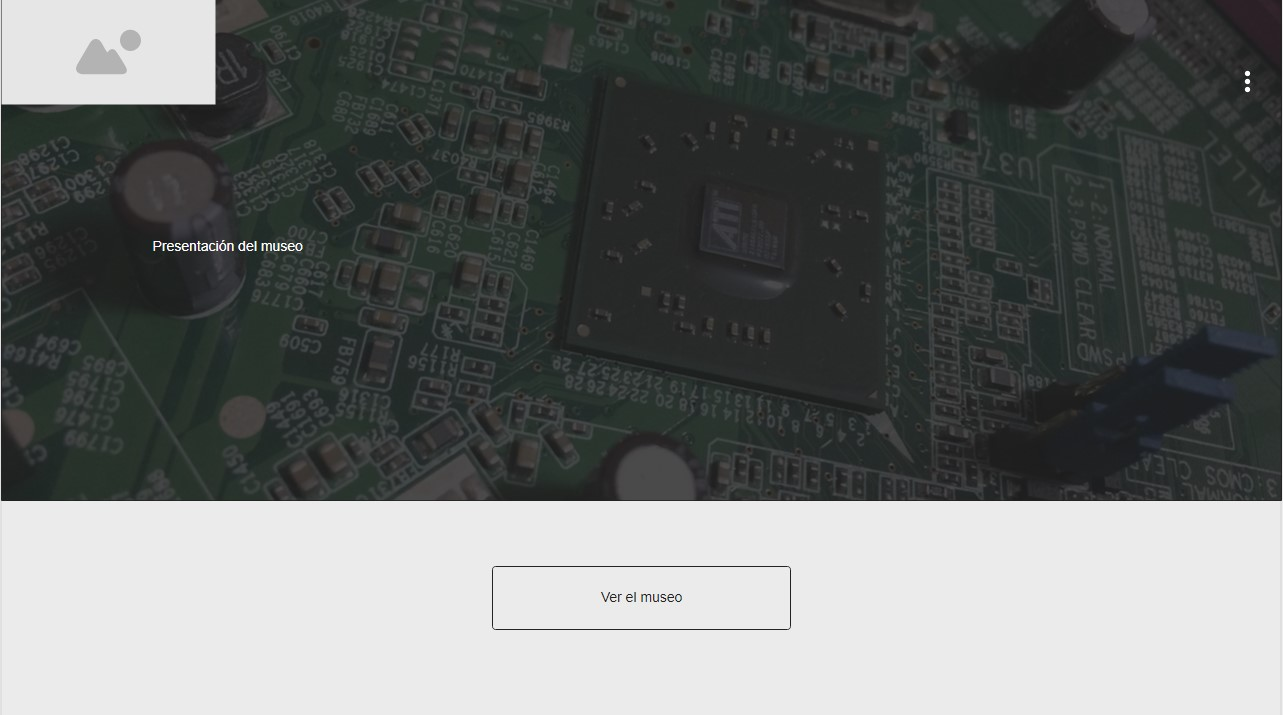
\includegraphics[scale=0.45]{homeIU}
\caption{Prototipo: Página de inicio}
\end{figure}
\paragraph*{Vista general del museo}\label{iu:timeline}
En la vista general del museo encontramos un menú lateral con filtros de búsqueda, y una sección principal que contiene una línea temporal con los periodos en los que se divide la historia de las CPUs.
\begin{figure}[H]
\centering
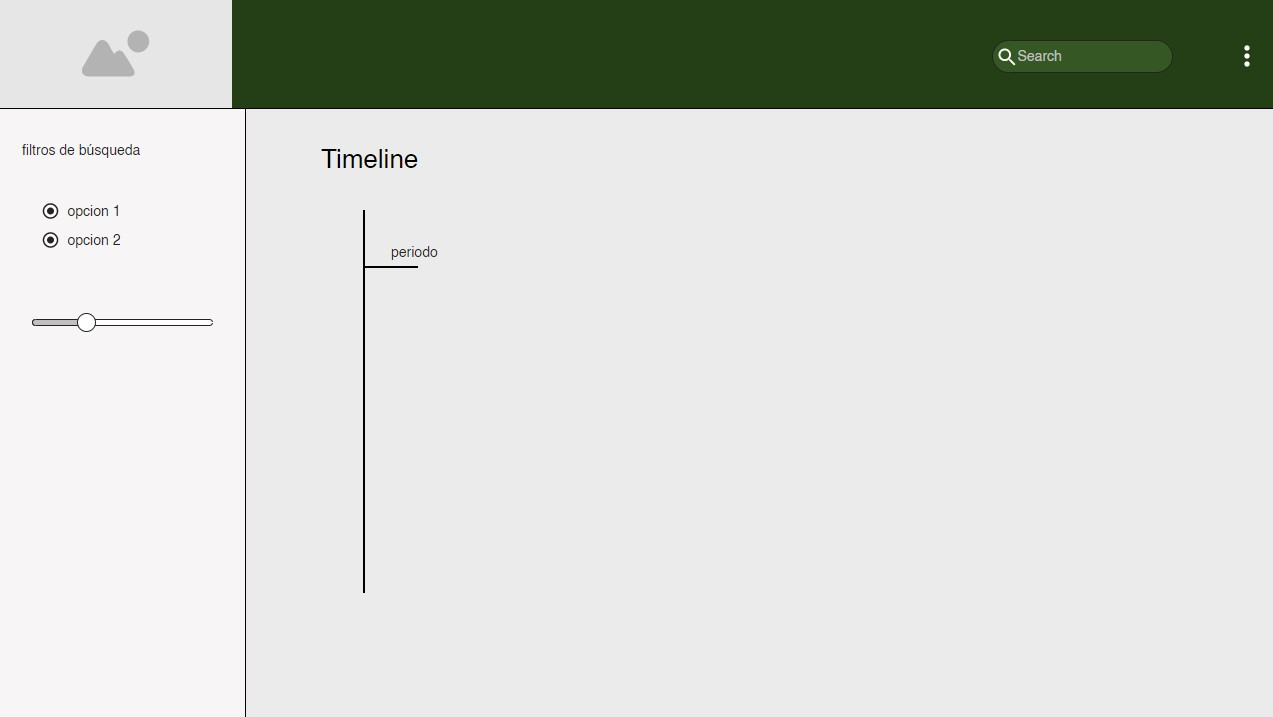
\includegraphics[scale=0.45]{museoIU}
\caption{Prototipo: Página de la vista general del museo}
\end{figure}
\paragraph*{Detalles del periodo}\label{iu:period-details}
En esta página hay un menú para volver a la vista general, y se muestran todos los detalles de un periodo (nombre, características, sistemas famosos de dicho periodo, etc.) y los componentes que pertenecen al mismo. 
\begin{figure}[H]
\centering
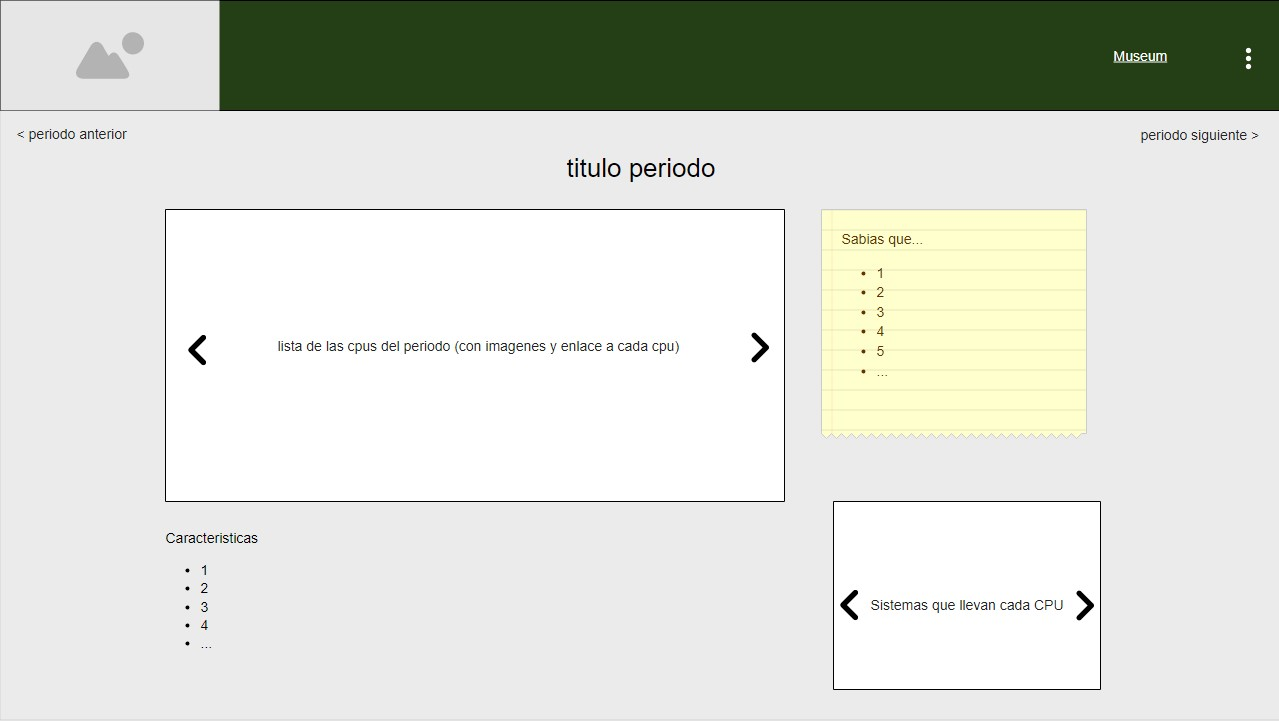
\includegraphics[scale=0.45]{periodoIU}
\caption{Prototipo: Página de detalles del periodo (museo)}
\end{figure}
\paragraph*{Detalles del componente}\label{iu:comp-details}
En esta página se muestra una galería de fotos del componente, la descripción del mismo, y un listado de características. En el menú de esta página hay un listado de componentes pertenecientes al mismo periodo.
\begin{figure}[H]
\centering
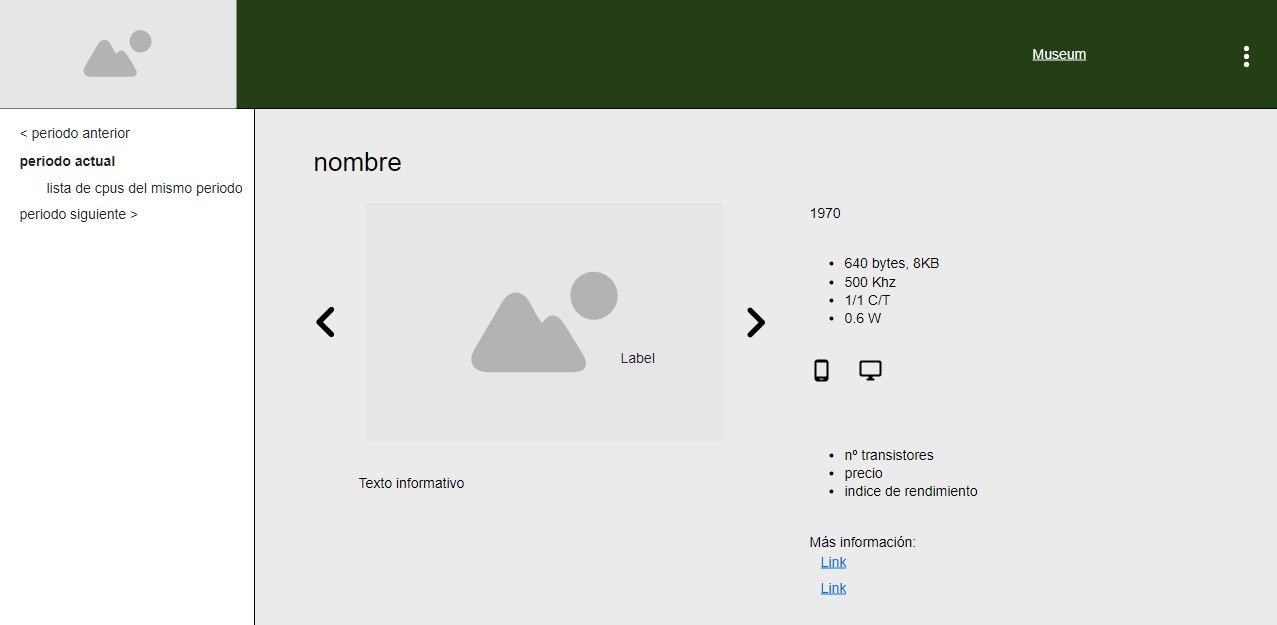
\includegraphics[scale=0.45]{piezaIU}
\caption{Prototipo: Página de detalles del componente (museo)}
\end{figure}

\subsubsection{Administración del museo}
A continuación, se muestran los prototipos inciales para la aplicación de administración del museo. En todas ellas, salvo en la de inicio de sesión, hay un menú lateral de navegación. 
\paragraph*{Iniciar sesión}\label{iu:login}
En esta página el administrador del sistema deberá introducir su usuario y contraseña para acceder al mismo.
\begin{figure}[H]
\centering
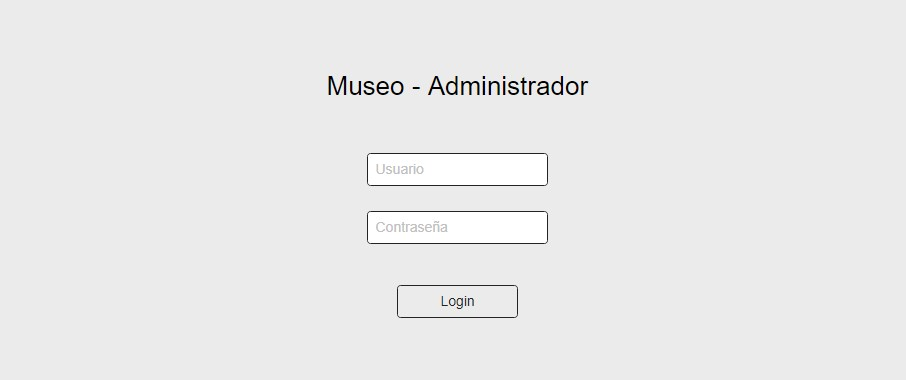
\includegraphics[scale=0.55]{loginIU}
\caption{Prototipo: Página de inicio de sesión}
\end{figure}
\paragraph*{Listado de periodos}\label{iu:list-periods}
En esta página se muestra un listado de los periodos existentes, con las opciones de acceder a cada uno, editarlo o eliminarlo.
\begin{figure}[H]
\centering
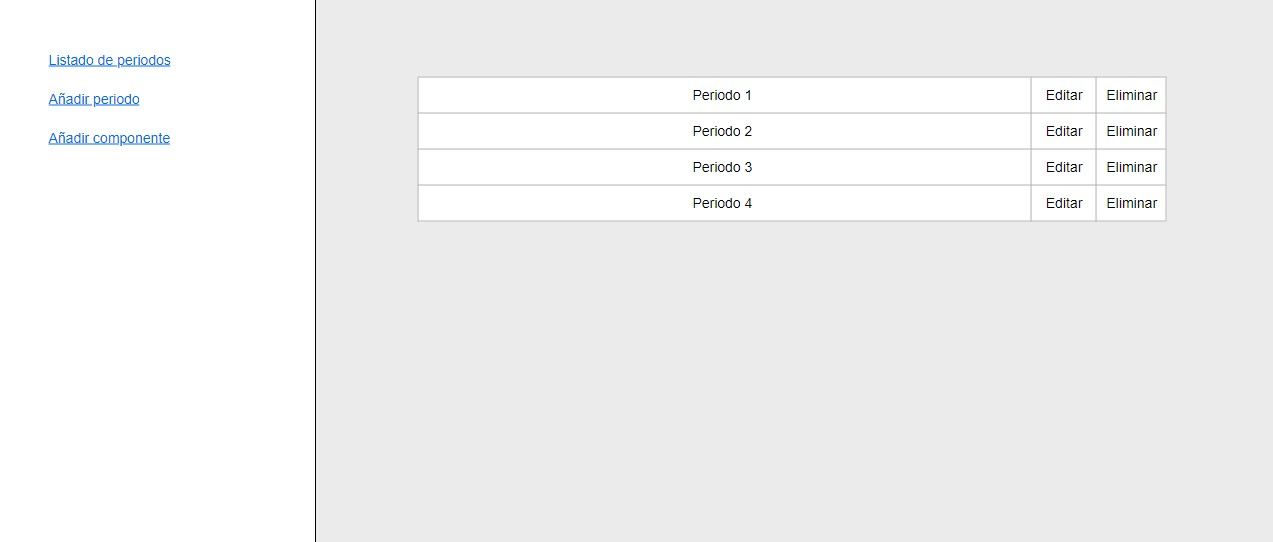
\includegraphics[scale=0.45]{listadoPeriodosIU}
\caption{Prototipo: Página de listado de periodos}
\end{figure}
\paragraph*{Periodo}\label{iu:period}
Esta página contiene los detalles de un periodo así como un listado de los componentes pertenecientes al mismo, ofreciendo la opción de acceder a ellos, editarlos o eliminarlos.
\begin{figure}[H]
\centering
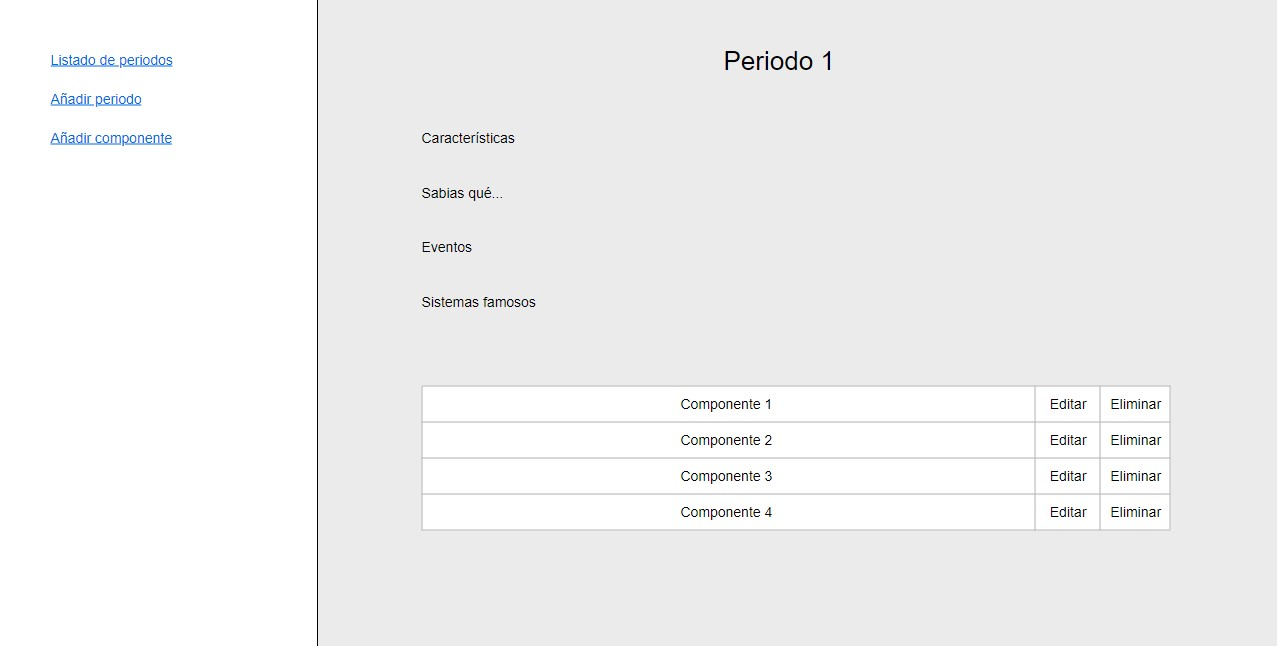
\includegraphics[scale=0.45]{periodoIU2}
\caption{Prototipo: Página de detalles de un periodo (admimnistración)}
\end{figure}
\paragraph*{Componente}\label{iu:my-comp}
En esta página se muestran los detalles correspondientes al componente.
\begin{figure}[H]
\centering
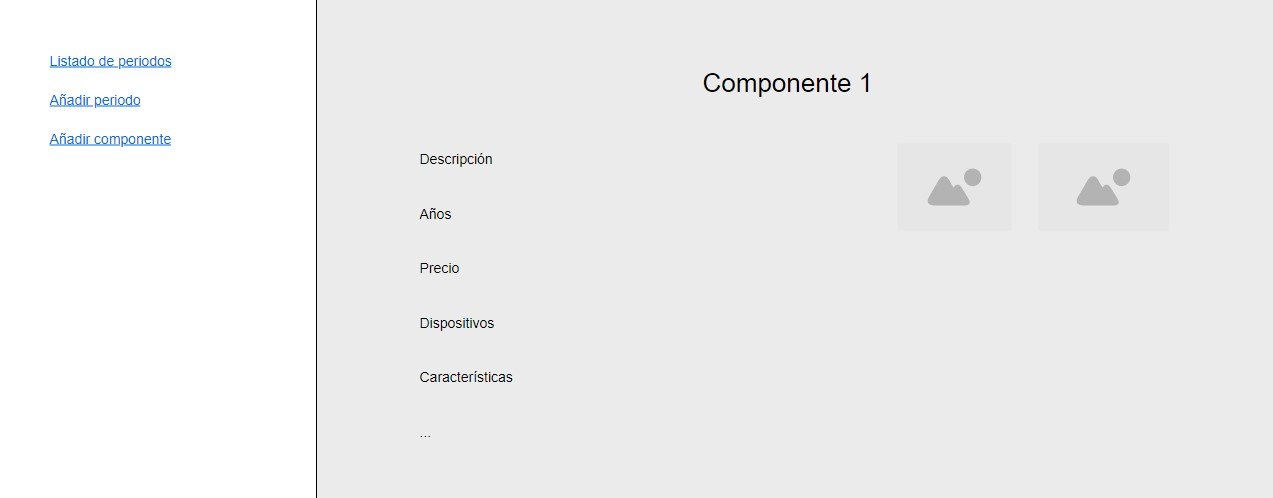
\includegraphics[scale=0.45]{compIU}
\caption{Prototipo: Página de detalles de un componente (admimnistración)}
\end{figure}
\paragraph*{Añadir/editar periodo}\label{iu:add-period}
Los formularios para añadir o editar un periodo son idénticos, con la única diferencia de que el formulario para editar ya tiene los campos completados con los valores existentes del periodo, por tanto solo se muestra una captura representando ambos.
\begin{figure}[H]
\centering
\includegraphics[scale=0.45]{añadirPeriodoIU}
\caption{Prototipo: Formulario para añadir o editar un periodo}
\end{figure}
\paragraph*{Añadir/editar componente}\label{iu:add-comp}
Con los formularios para añadir o editar un componente ocurre igual que con los del periodo ya mencionados.
\begin{figure}[H]
\centering
\includegraphics[scale=0.45]{añadirCompIU}
\caption{Prototipo: Formulario para añadir o editar un componente}
\end{figure}



%\subsection{Descripción del Comportamiento de la Interfaz} 

\subsection{Diagrama de Navegabilidad}
A continuación se presentan dos diagramas de navegabilidad, correspondientes a las dos aplicaciones web que constituyen el sistema.
\subsubsection{Museo}
\begin{figure}[H]
\centering
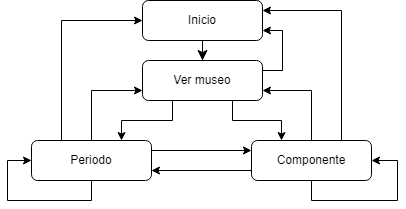
\includegraphics[scale=0.7]{nav-museo}
\caption{Diagrama de navegabilidad del museo}
\end{figure}

\subsubsection{Administración del museo}
\begin{figure}[H]
\centering
\centerline{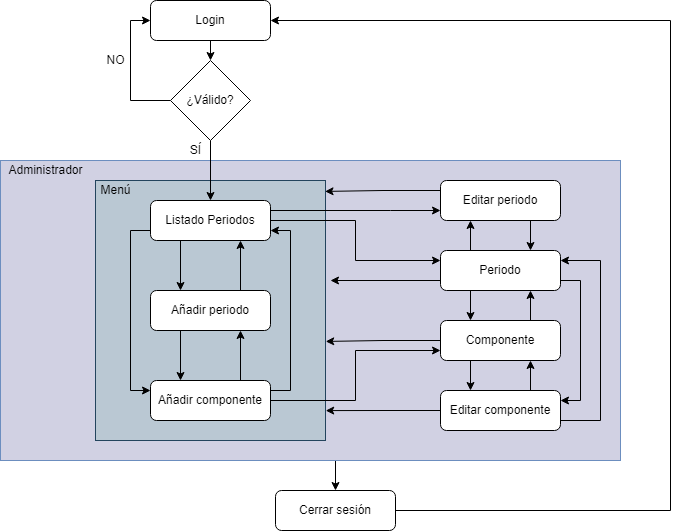
\includegraphics[scale=0.7]{nav-admin}}
\caption{Diagrama de navegabilidad de la administración del museo}
\end{figure}

\newpage
\section{ASI 10: ESPECIFICACIÓN DEL PLAN DE PRUEBAS}

\input{7-Diseño}
\newpage
\chapter{CONSTRUCCIÓN DEL SISTEMA DE INFORMACIÓN}
	\vspace{2cm}	
	\begin{center}
	{\Large \textbf{FASE DE DESARROLLO} \par}
	\end{center}
	\vspace{5cm}
	
	\begin{center}
	\Huge \textbf{CSI}\par
	\end{center}

\newpage


\section{CSI 1: PREPARACIÓN DEL ENTORNO DE GENERACIÓN Y CONSTRUCCIÓN}

\subsection{Estándares y normas seguidos}
\subsubsection{Angular Style Guide}
La guía de estilos de Angular\cite{AngularSG} es un conjunto de recomendaciones sobre la sintaxis, estructura y convenciones de código en proyectos de Angular.
\subsubsection{HTML5}
HTML5 es la versión más reciente y la actualmente usada de HTML, y está estandarizada por el W3C (World Wide Web Consortium).
\subsubsection{CSS}
Hojas de estilos estandarizadas por el W3C.
\subsubsection{PHP Code Style Guide}
La guía de estilos de PHP\cite{PhpSG} contiene normas de código y buenas prácticas.

\subsection{Lenguajes de programación}
\subsubsection{TypeScript}
TypeScript es un lenguaje de programación de código abierto desarrollado por Microsoft. Extiende JavaScript añadiendo la definición de tipos estáticos.
\subsubsection{HTML}
HTML (HyperText Markup Language) es un lenguaje de marcado utilizado en la elaboración de páginas web.
\subsubsection{CSS}
CSS (Cascading Style Sheets) es un lenguaje de diseño gráfico que permite modificar la presentación de los elementos definidos en los documentos HTML.
\subsubsection{PHP}
PHP es un lenguaje de programación utilizado en el desarrollo web que es procesado en el lado del servidor.
\subsubsection{SQL}
SQL (Structured Query Language) es un lenguaje de consultas utilizado para leer, insertar, actualizar o eliminar datos de la base de datos relacional utilizada. 
\subsection{Herramientas y programas usados para el desarrollo}
\subsubsection{Visual Studio Code}
Visual Studio Code es un editor de código fuente desarrollado por Microsoft, gratuito y de código abierto. Tiene soporte integrado para TypeScript y Node.js, extensiones para otros lenguajes como PHP. También cuenta con soporte para depuración, control integrado de Git e \textit{IntelliSense}, una función de autocompletado de código\cite{VSCode}.
\begin{figure}[H]
	\centering
	
\includegraphics[scale=0.05]{vscode}
	\caption{Logo de Visual Studio Code}
\end{figure}
\subsubsection{XAMPP}
XAMPP es una distribución de Apache gratuita que contiene MariaDB, PHP y Perl\cite{Xampp}. Fue usado inicialmente para trabajar con la base de datos y los PHP necesarios, pero una vez configurado el servidor Ubuntu 20.04 dejó de ser necesario.
\begin{figure}[H]
	\centering
	
\includegraphics[scale=0.3]{xampp}
	\caption{Logo de XAMPP}
\end{figure}
\subsubsection{MobaXTerm}
MobaXTerm permite trabajar con herramientas de red remotas, como SSH, utilizando una terminal Unix desde Windows. Se ha usado para configurar el servidor Ubuntu 20.04 que aloja el servidor MySQL con la base de datos del sistema, y el servidor Apache con los PHP que se utilizan para trabajar con esta base de datos.
\begin{figure}[H]
	\centering
	\includegraphics[scale=0.5]{MobaXTerm}
	\caption{Logo de MobaXTerm}
\end{figure}

\subsubsection{Git}
Git es un software de control de versiones gratuito y de código abierto, diseñado para gestionar los cambios de un repositorio\cite{Git}.
\begin{figure}[H]
	\centering
	
\includegraphics[scale=0.2]{git}
	\caption{Logo de Git}
\end{figure}

\newpage
\section{CSI 2: GENERACIÓN DEL CÓDIGO DE LOS COMPONENTES Y PROCEDIMIENTOS}

\textcolor[rgb]{0.65,0.16,0}{Ejemplos de tablas descripción de clases}

\begin{table}[H]
\vspace{-4mm}
  \centering
  \caption{Descripción de diseño de LoginScreen}
    \begin{tabular}{p{8.645em}rr}
    \toprule
    \rowcolor[rgb]{ .851,  .886,  .953} \multicolumn{3}{p{31.285em}}{\textbf{LoginScreen}} \\
    \midrule
    \rowcolor[rgb]{ .949,  .949,  .949} \multicolumn{3}{p{31.285em}}{\textbf{Descripción}} \\
    \midrule
    \multicolumn{3}{p{31.285em}}{Es la encargada de las acciones y la renderización de la pantalla de inicio de sesión.} \\
    \midrule
    \rowcolor[rgb]{ .906,  .902,  .902} \multicolumn{3}{p{31.285em}}{\textbf{Atributos propuestos}} \\
    \midrule
    \multicolumn{3}{p{31.285em}}{-} \\
    \midrule
    \rowcolor[rgb]{ .906,  .902,  .902} \multicolumn{3}{p{31.285em}}{\textbf{Métodos propuestos}} \\
    \midrule
    \textbf{signInWithGoogle} & \multicolumn{2}{p{22.64em}}{Hace una llamada al objeto Fire para el inicio de sesión con Firebase authentication mediante una cuenta de Google.} \\
    \midrule
    \textbf{render} & \multicolumn{2}{r}{} \\
    \bottomrule
    \end{tabular}%
\end{table}%


\begin{table}[htbp]
  \centering
  \caption{Descripción de diseño de HomeScreen}
    \begin{tabular}{p{10em}rr}
    \toprule
    \rowcolor[rgb]{ .851,  .886,  .953} \multicolumn{3}{p{31.285em}}{\textbf{HomeScreen}} \\
    \midrule
    \rowcolor[rgb]{ .949,  .949,  .949} \multicolumn{3}{p{31.285em}}{\textbf{Descripción}} \\
    \midrule
    \multicolumn{3}{p{31.285em}}{Es la encargada de las acciones y la renderización de la pantalla de emergencia.} \\
    \midrule
    \rowcolor[rgb]{ .906,  .902,  .902} \multicolumn{3}{p{31.285em}}{\textbf{Atributos propuestos}} \\
    \midrule
    \multicolumn{3}{p{31.285em}}{-} \\
    \midrule
    \rowcolor[rgb]{ .906,  .902,  .902} \multicolumn{3}{p{31.285em}}{\textbf{Métodos propuestos}} \\
    \midrule
    \textbf{componentWillMount} & \multicolumn{2}{r}{} \\
    \midrule
    \textbf{emergencyCalling} & \multicolumn{2}{p{21.285em}}{Es el método encargado de redirigir la aplicación hacia el marcador con el 112 marcado.} \\
    \midrule
    \textbf{warnProtectors} & \multicolumn{2}{p{21.285em}}{[Falta implementar] Es el encargado de generar un mensaje de aviso a los protectores creando notificaciones push.} \\
    \midrule
    \textbf{render} & \multicolumn{2}{r}{} \\
    \bottomrule
    \end{tabular}%
\end{table}%

\newpage
\section{CSI 3: EJECUCIÓN DE LAS PRUEBAS UNITARIAS}


\newpage
\section{CSI 4: EJECUCIÓN DE LAS PRUEBAS DE INTEGRACIÓN}


\newpage
\section{CSI 5: EJECUCIÓN DE LAS PRUEBAS DEL SISTEMA}

\subsection{Prueba de Usabilidad}

\subsection{Pruebas de Accesibilidad} 
 
\subsubsection{Revisión Preliminar} 

\subsubsection{Evaluación de Conformidad} 

\subsubsection{Checklist del WCAG 2.1} 

\subsubsection{Accesibilidad con Dispositivos Móviles} 


\newpage
\section{CSI 6: ELABORACIÓN DE LOS MANUALES DE USUARIO}

\subsection{Manual de Instalación} 
En este manual se detallarán los pasos necesarios para realizar las instalaciones necesarias para la ejecución del sistema.\par
En primer lugar, es necesario instalar NodeJS (se puede descargar en \url{https://nodejs.org/en/download/}) y reiniciar el sistema, ya que con esta instalación se ha cambiado la configuración de variables del PATH.\par
Para los siguientes pasos, es necesario el uso de la terminal del sistema.\par
Usando npm, el gestor de paquetes de NodeJS, hay que instalar Angular CLI. Para ello hay que ejecutar el comando \textit{npm install -g @angular/cli}.
\begin{figure}[H]
\centering

\includegraphics[scale=1]{npmangularcli}
\caption{Instalación de Angular CLI}
\end{figure}
Por último, desde la carpeta que ubica tanto el proyecto del museo (museo-eii) como el de la administración (museo-eii-admin), se ejecuta el comando \textit{npm install} para instalar los paquetes necesarios.
\begin{figure}[H]
\centering
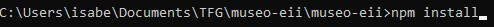
\includegraphics[scale=1]{npminstallmuseo}
\caption{Instalación de los paquetes del proyecto del museo}
\end{figure}
\begin{figure}[H]
\centering
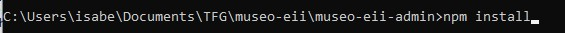
\includegraphics[scale=1]{npminstalladmin}
\caption{Instalación de los paquetes del proyecto de administración}
\end{figure}


\subsection{Manual de Ejecución} 
Una vez completada la instalación siguiendo los pasos descritos en el apartado anterior, se pueden ejecutar ambas aplicaciones utilizando el comando \textit{ng serve -o}, \textit{npm start} o \textit{npm run ng serve -o}. Esto hará que la aplicación esté disponible en \url{http://localhost:4200}.
\begin{figure}[H]
\centering
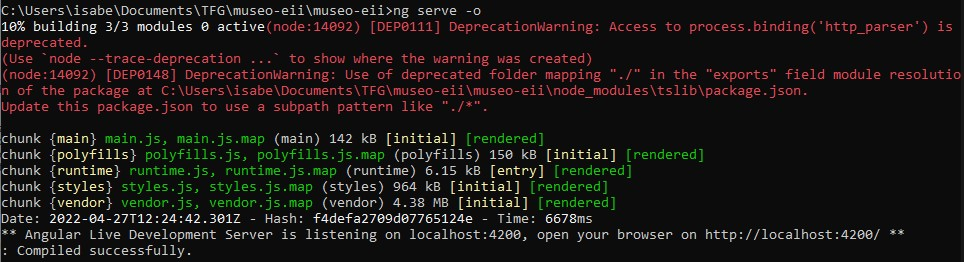
\includegraphics[scale=0.65]{ngservemuseo}
\caption{Ejecución de la aplicación del museo}
\end{figure}
\begin{figure}[H]
\centering
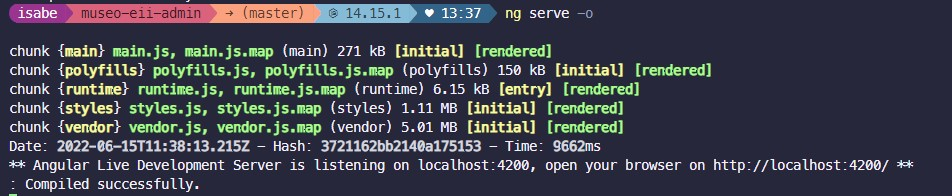
\includegraphics[scale=0.65]{ngserveadmin}
\caption{Ejecución de la aplicación de administración}
\end{figure}


\subsection{Manual de Usuario} 
\subsubsection{Museo}
Al acceder a la web observamos la página de inicio. La parte superior de esta página está presente en toda la aplicación web y, por orden de izquierda a derecha, observamos:
\begin{itemize}
	\item El logo de la escuela, que redirige a esta página de inicio.
	\item Museo, que redirige a la vista general del museo.
	\item Acerca de.
	\item Un selector de idioma, que permite cambiar entre inglés y español.
\end{itemize}
La parte inferior, que contiene enlaces a las redes sociales de la escuela, también está presente en toda la aplicación web.\par
En la parte central se encuentra el contenido específico de la página de inicio: una bienvenida a la página web y un botón que nos dirige a la vista general del museo.
\begin{figure}[H]
\centering
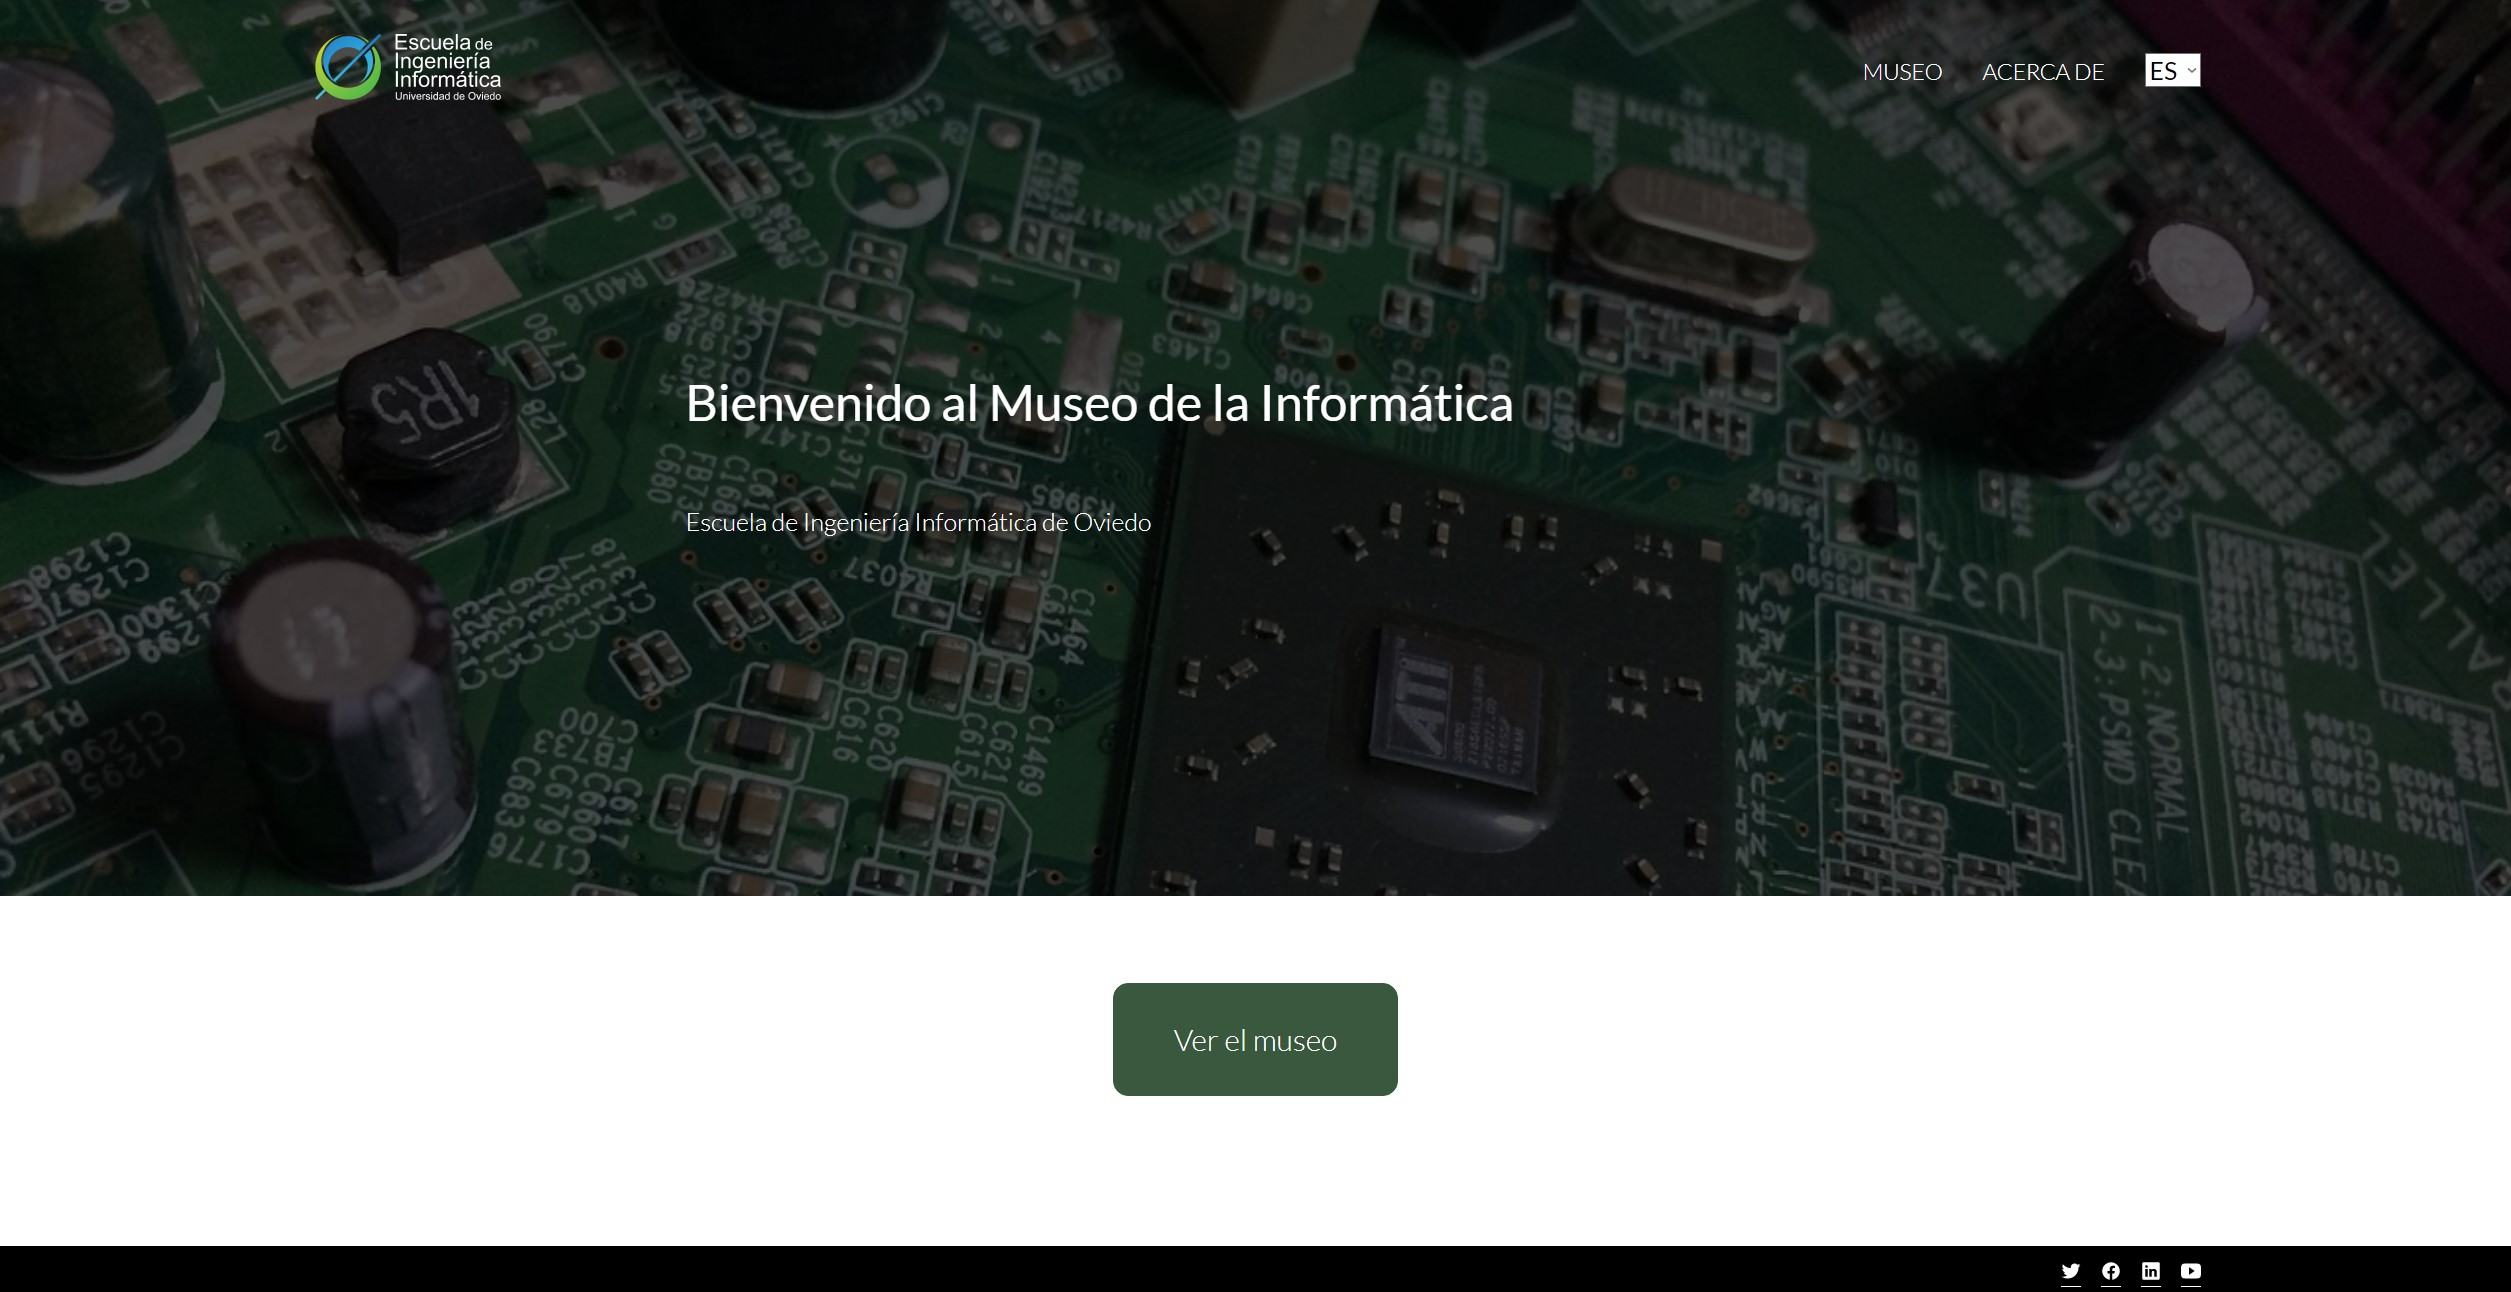
\includegraphics[scale=0.25]{homeIUDef}
\caption{Manual de usuario: Inicio}
\end{figure}
En la vista general del museo hay una línea temporal y filtros de búsqueda.\par
En cada elemento de la línea temporal se muestra el nombre del periodo con un enlace al mismo, los años que comprende dicho periodo, y los nombres de los componentes pertenecientes al periodo, también con enlaces a cada uno de ellos.\par
La búsqueda puede realizarse por años o por nombre. Se puede filtrar por años mediante la barra deslizadora, y se mostrarán entonces todos aquellos periodos que, parcialmente o en su totalidad, tengan componentes pertenecientes a esos años. La búsqueda por nombre se realiza tras escribir en el recuadro de búsqueda y pulsar la tecla \textit{Enter}, y el resultado será aquellos periodos cuyo nombre o el nombre de alguno de sus componentes contenga el texto buscado.
\begin{figure}[H]
\centering
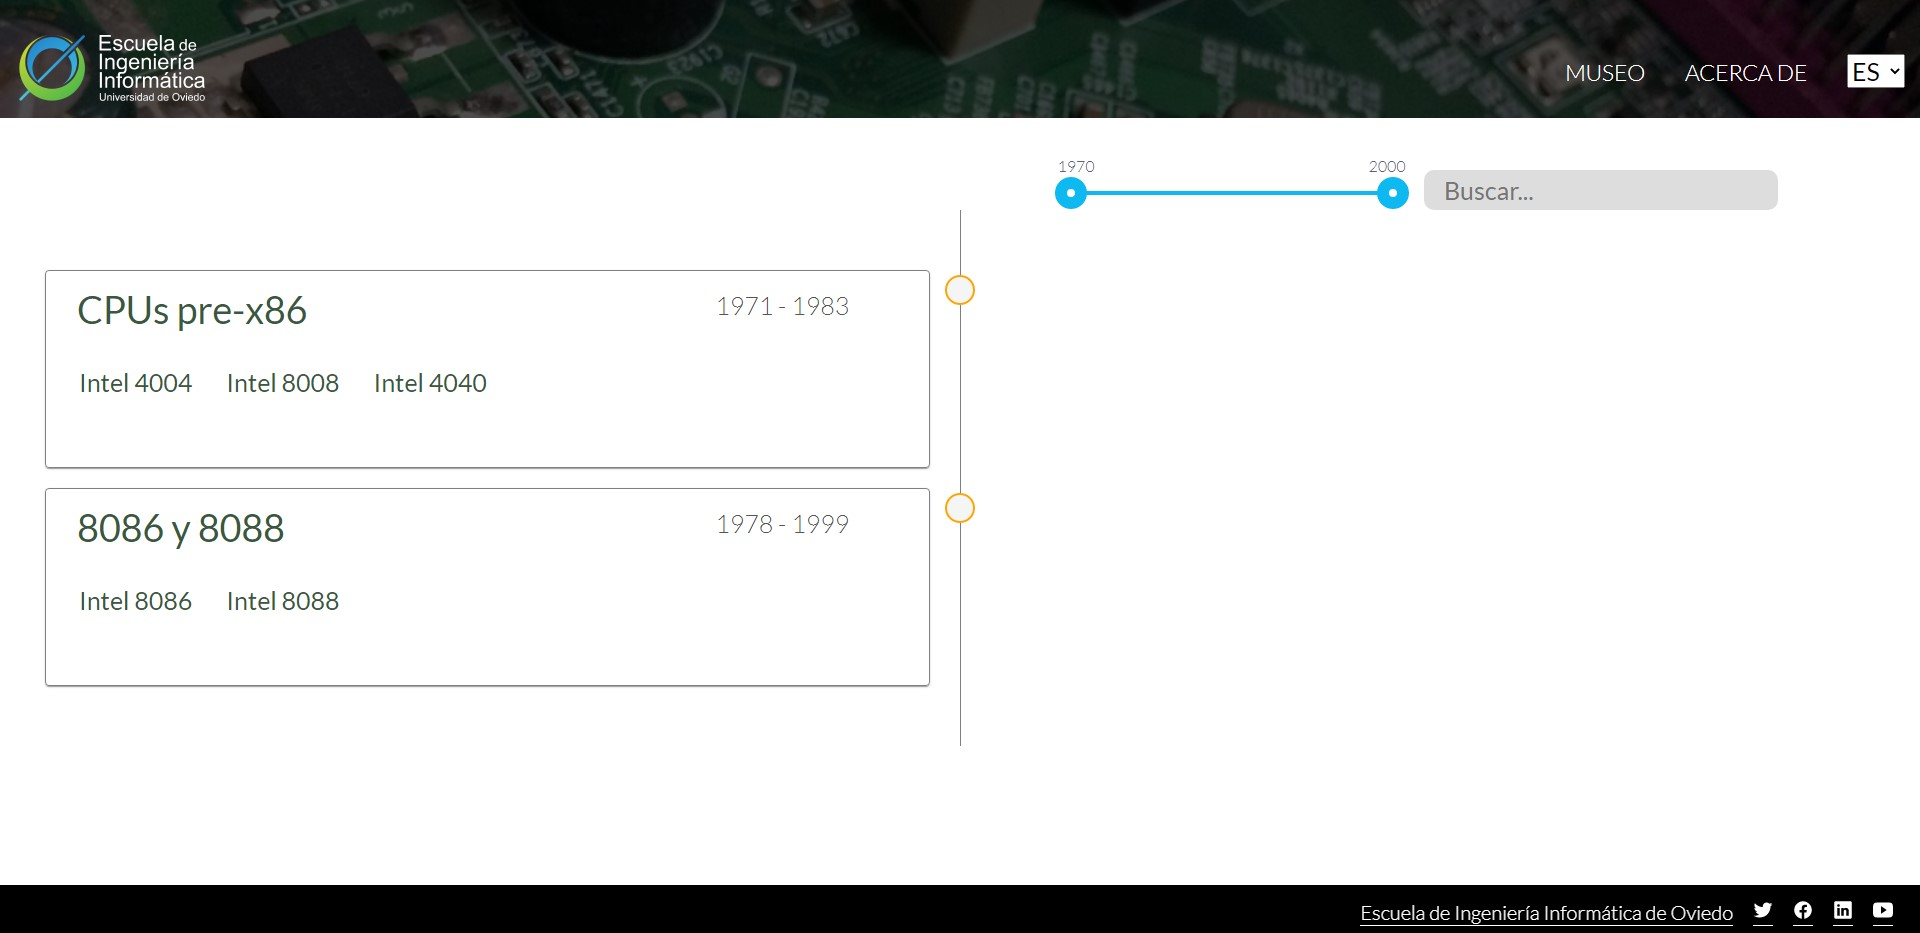
\includegraphics[scale=0.25]{museoIUDef}
\caption{Manual de usuario: Vista general del museo}
\end{figure}
Al entrar en un periodo, en la parte superior podemos ver un menú, en la izquierda se mostraría el periodo anterior cronológicamente, y en la izquierda el periodo siguiente (si existen). El contenido principal de la página son los detalles del periodo: nombre, características, una lista de curiosidades (sabías que...), eventos informáticos ocurridos en esos años, los componentes pertenecientes al periodo (mostrando una imagen y el nombre, con un enlace al componente), y una serie de sistemas famosos que llevan esos componentes. 
\begin{figure}[H]
\centering
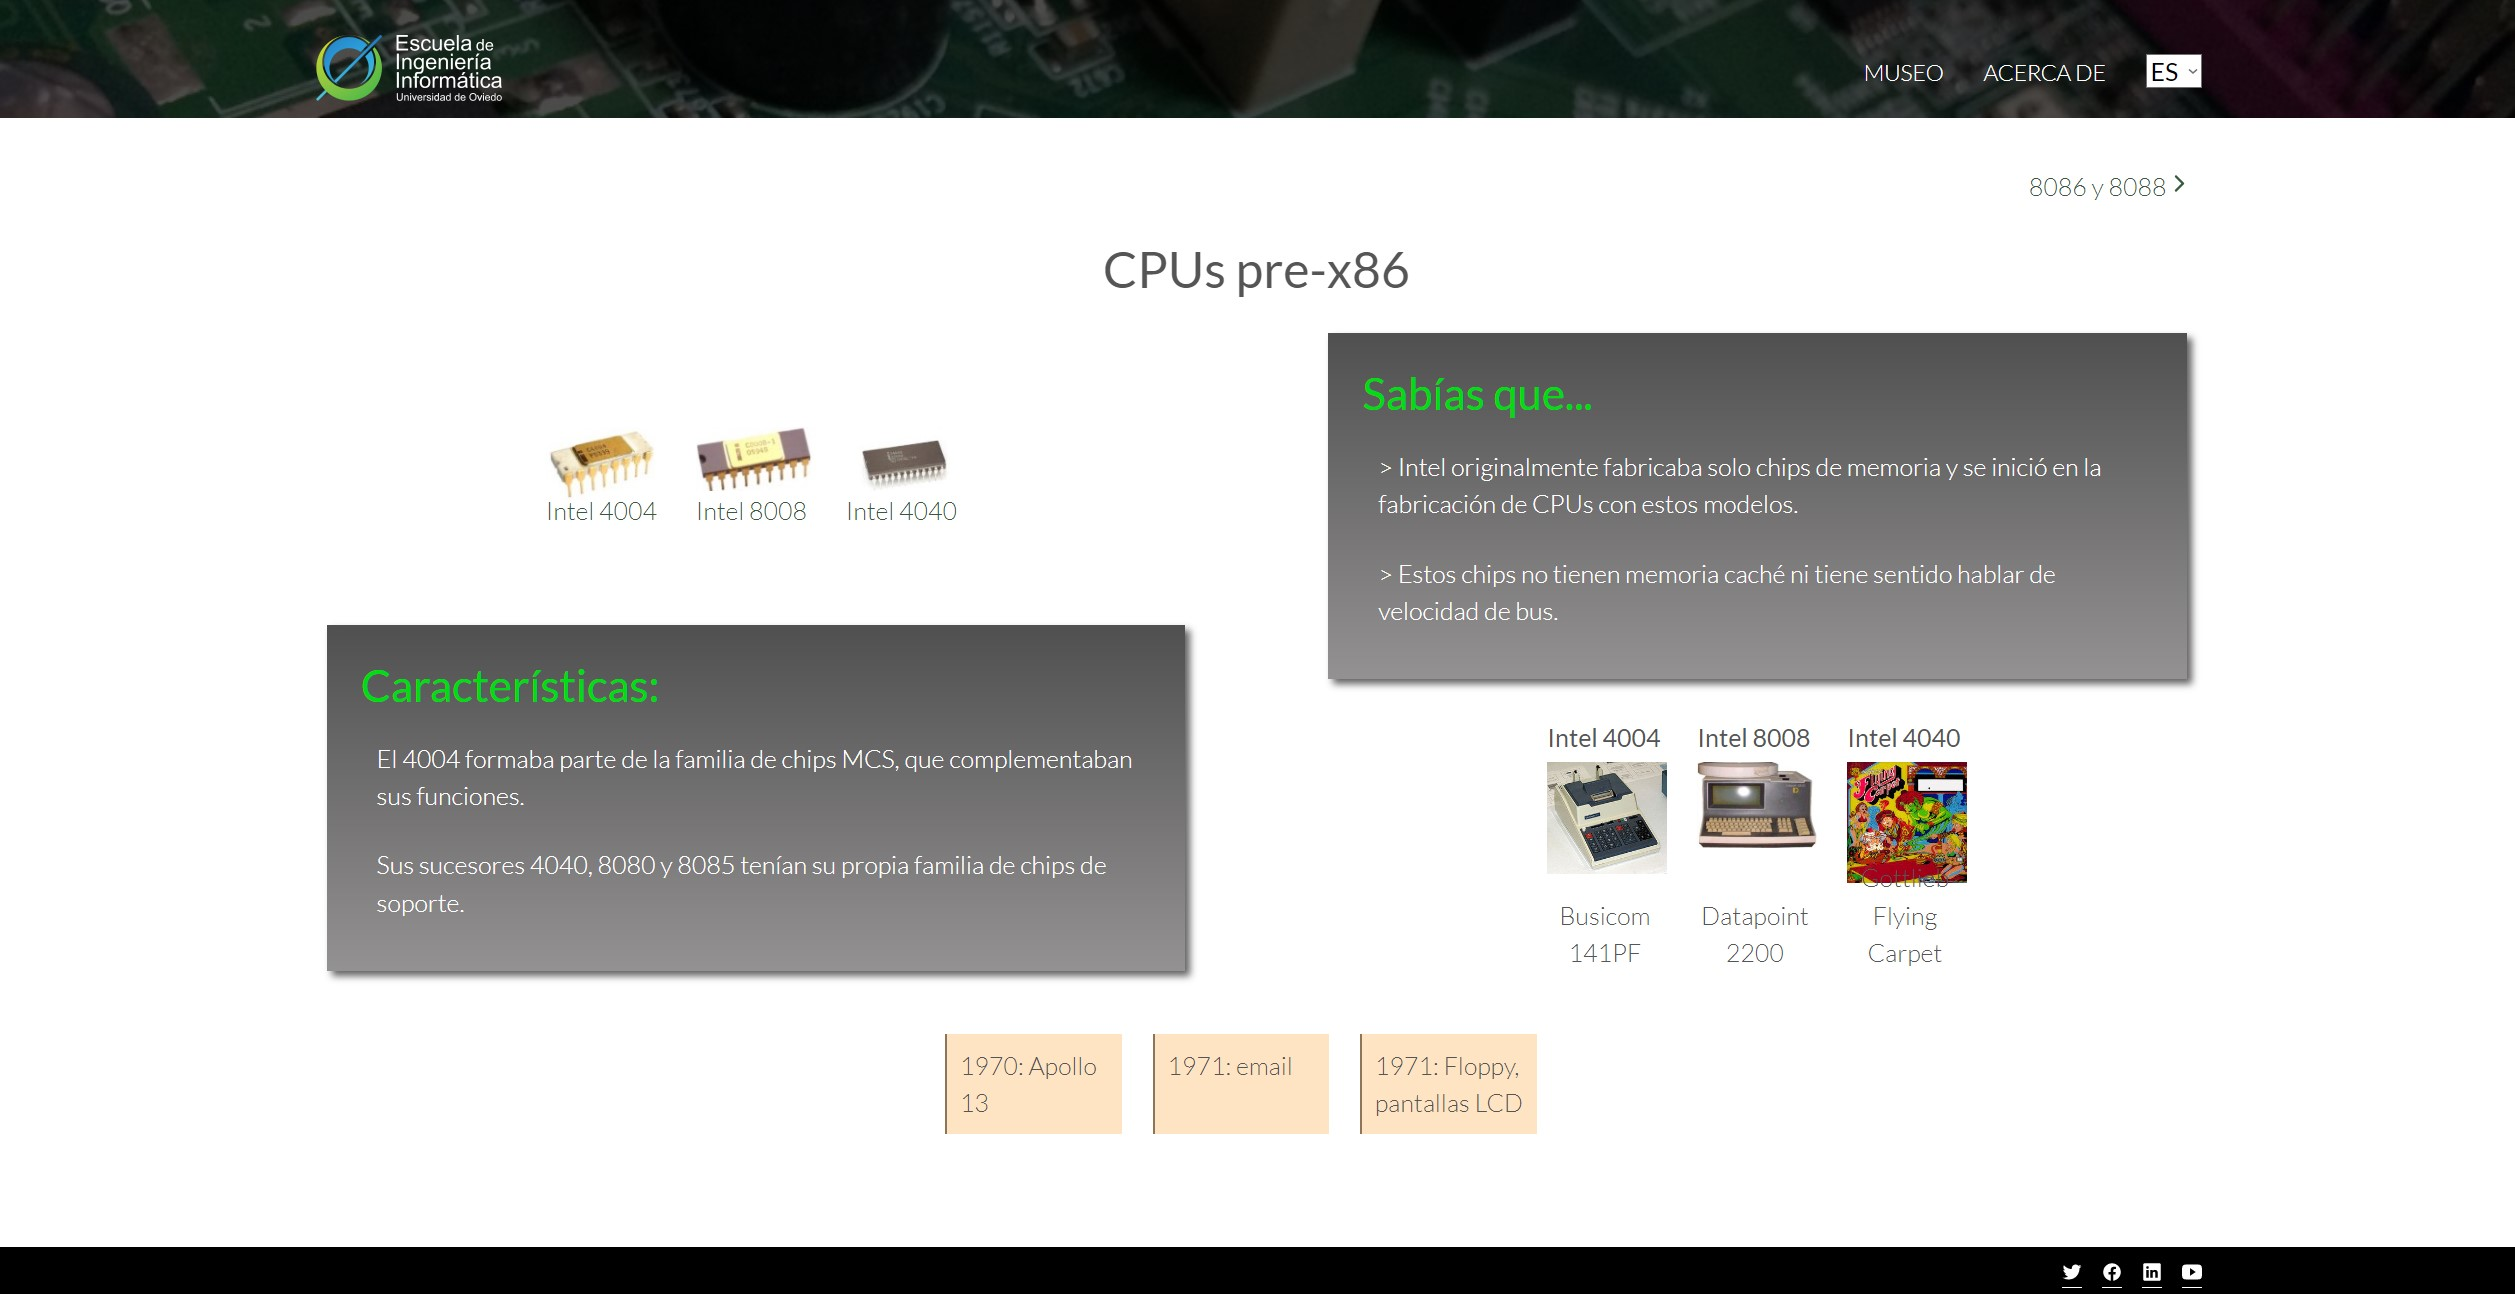
\includegraphics[scale=0.25]{periodoIUDef}
\caption{Manual de usuario: Detalles del periodo (museo)}
\end{figure}
Por último, al acceder a un componente, podemos ver una galería de fotos que se abrirán en grande al pulsar sobre ellas, una descripción del componente y un listado de características. Además, en el lateral izquierdo hay un menú que permite navegar entre periodos (ver el anterior, el actual y el siguiente) y entre los componentes del periodo actual.
\begin{figure}[H]
\centering
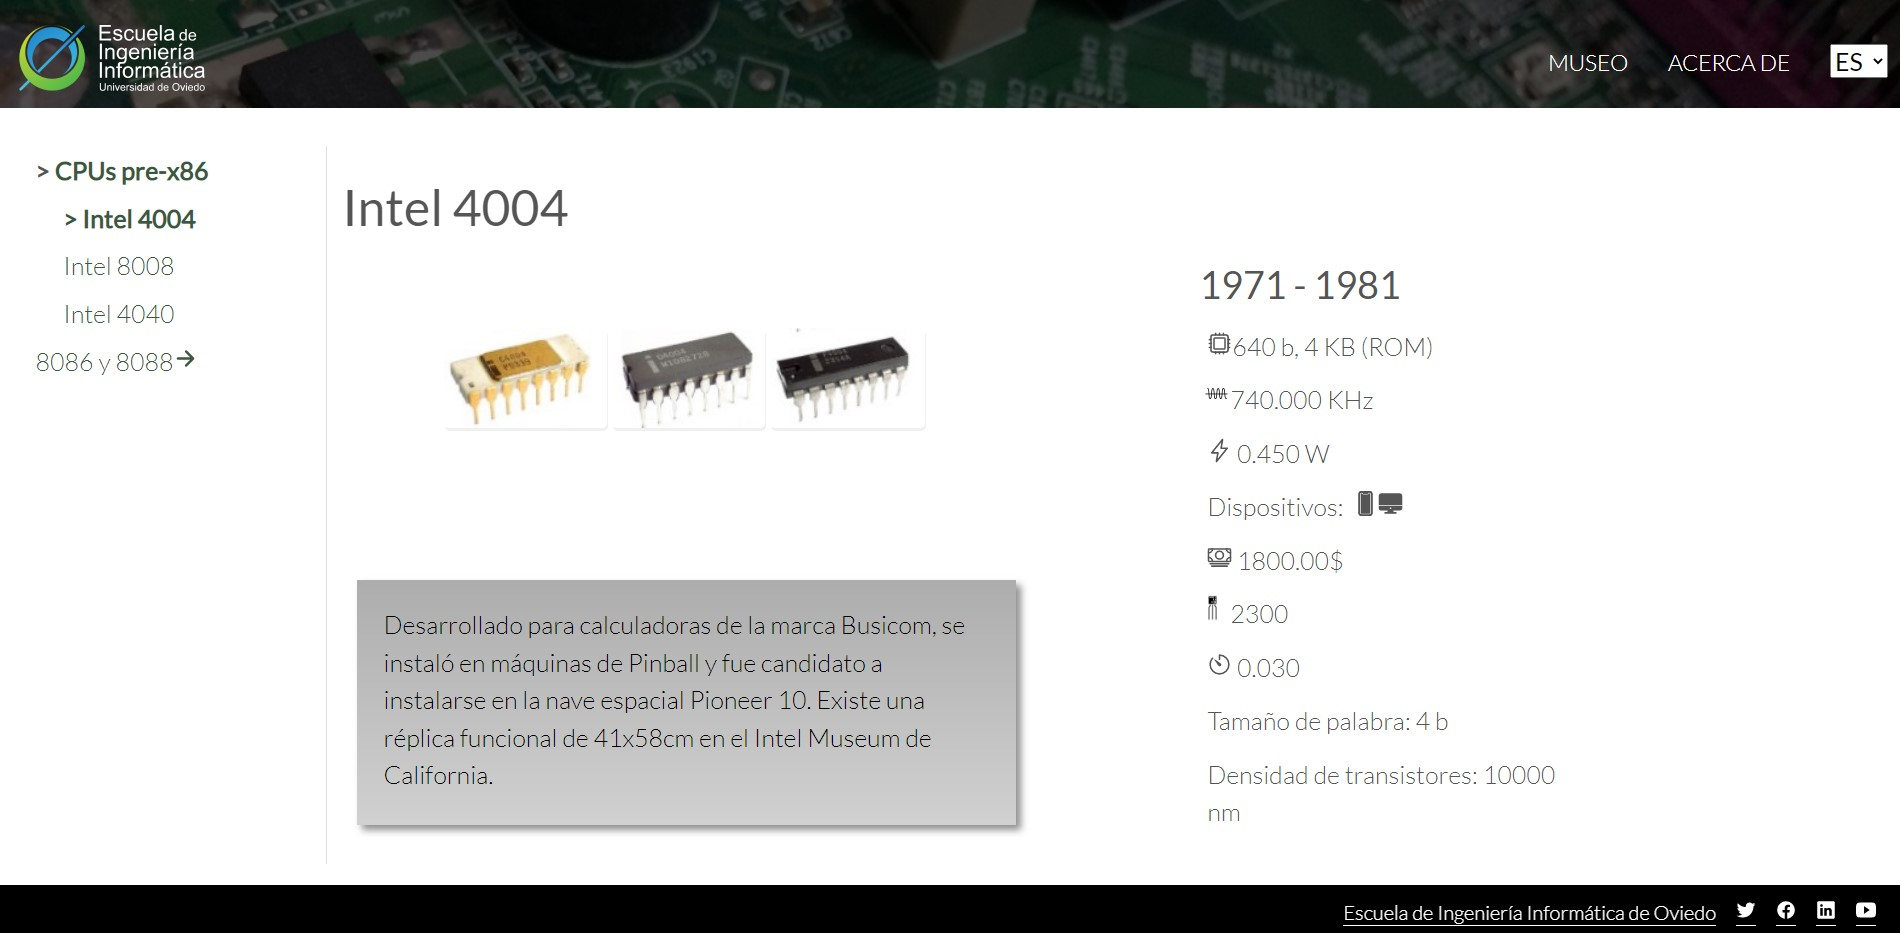
\includegraphics[scale=0.25]{piezaIUDef}
\caption{Manual de usuario: Detalles del componente (museo)}
\end{figure}

\subsubsection{Administración del museo}
Al entrar a la web de administración del museo nos encontramos con el inicio de sesión. Es necesario indicar el correo electrónico y la contraseña para acceder.
\begin{figure}[H]
\centering
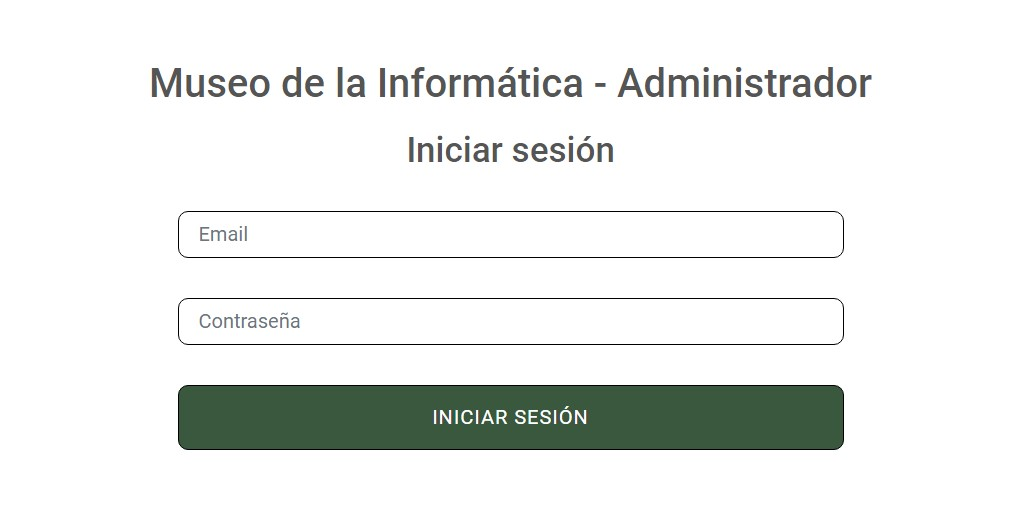
\includegraphics[scale=0.45]{loginIUDef}
\caption{Manual de usuario: Inicio de sesión}
\end{figure}
Lo primero que se muestra una vez iniciada la sesión es un listado de los periodos existentes, mostrando sus nombres con un enlace a cada uno de ellos, y permitiendo editar y eliminar cada periodo. Eliminar un periodo borrará también los componentes asociados al mismo, para ello se mostrará un aviso y se pedirá confirmación. En el lateral izquierdo hay un menú que se incluye en todas las páginas de la aplicación, desde el que se puede acceder a este listado de periodos, y a los formularios para añadir periodos y componentes.
\begin{figure}[H]
\centering

\includegraphics[scale=0.35]{listadoPeriodosIUDef}
\caption{Manual de usuario: Listado de periodos}
\end{figure}
Los detalles de un periodo y del componente muestran los mismos datos explicados anteriormente en el manual de usuario del museo, con la diferencia de en que cada una de estas páginas se muestra una opción para editar el periodo o el componente que estemos visualizando, y en el listado de componentes del periodo también se da la opción de editar o eliminar cada uno de ellos.
\begin{figure}[H]
\centering
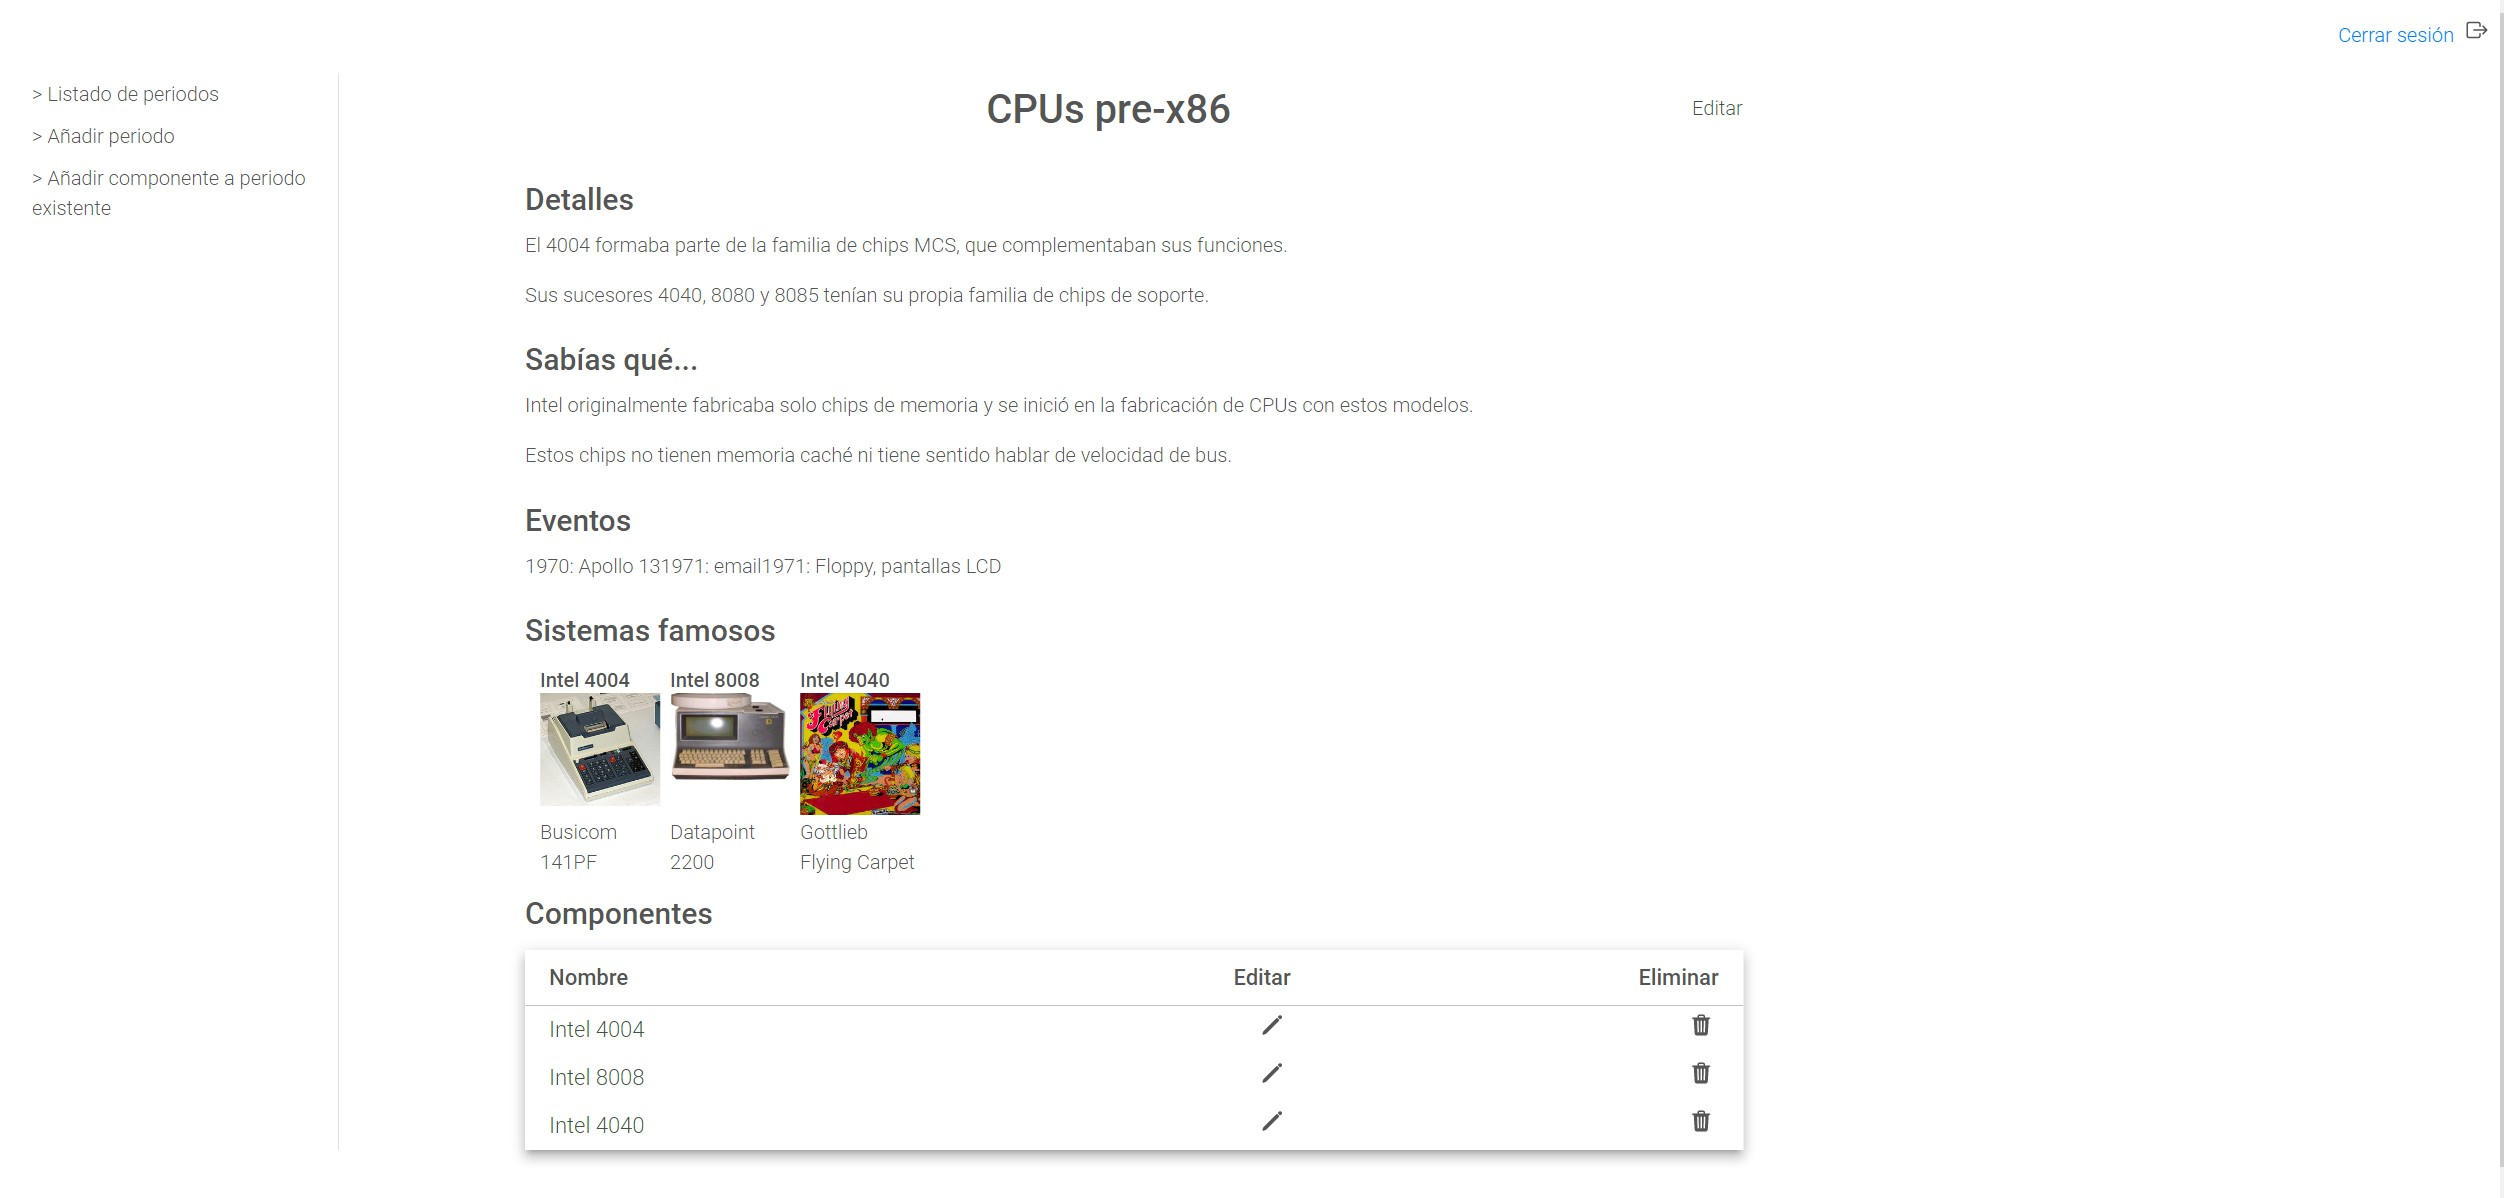
\includegraphics[scale=0.35]{periodoIU2Def}
\caption{Manual de usuario: Detalles de un periodo (administración)}
\end{figure}
\begin{figure}[H]
\centering
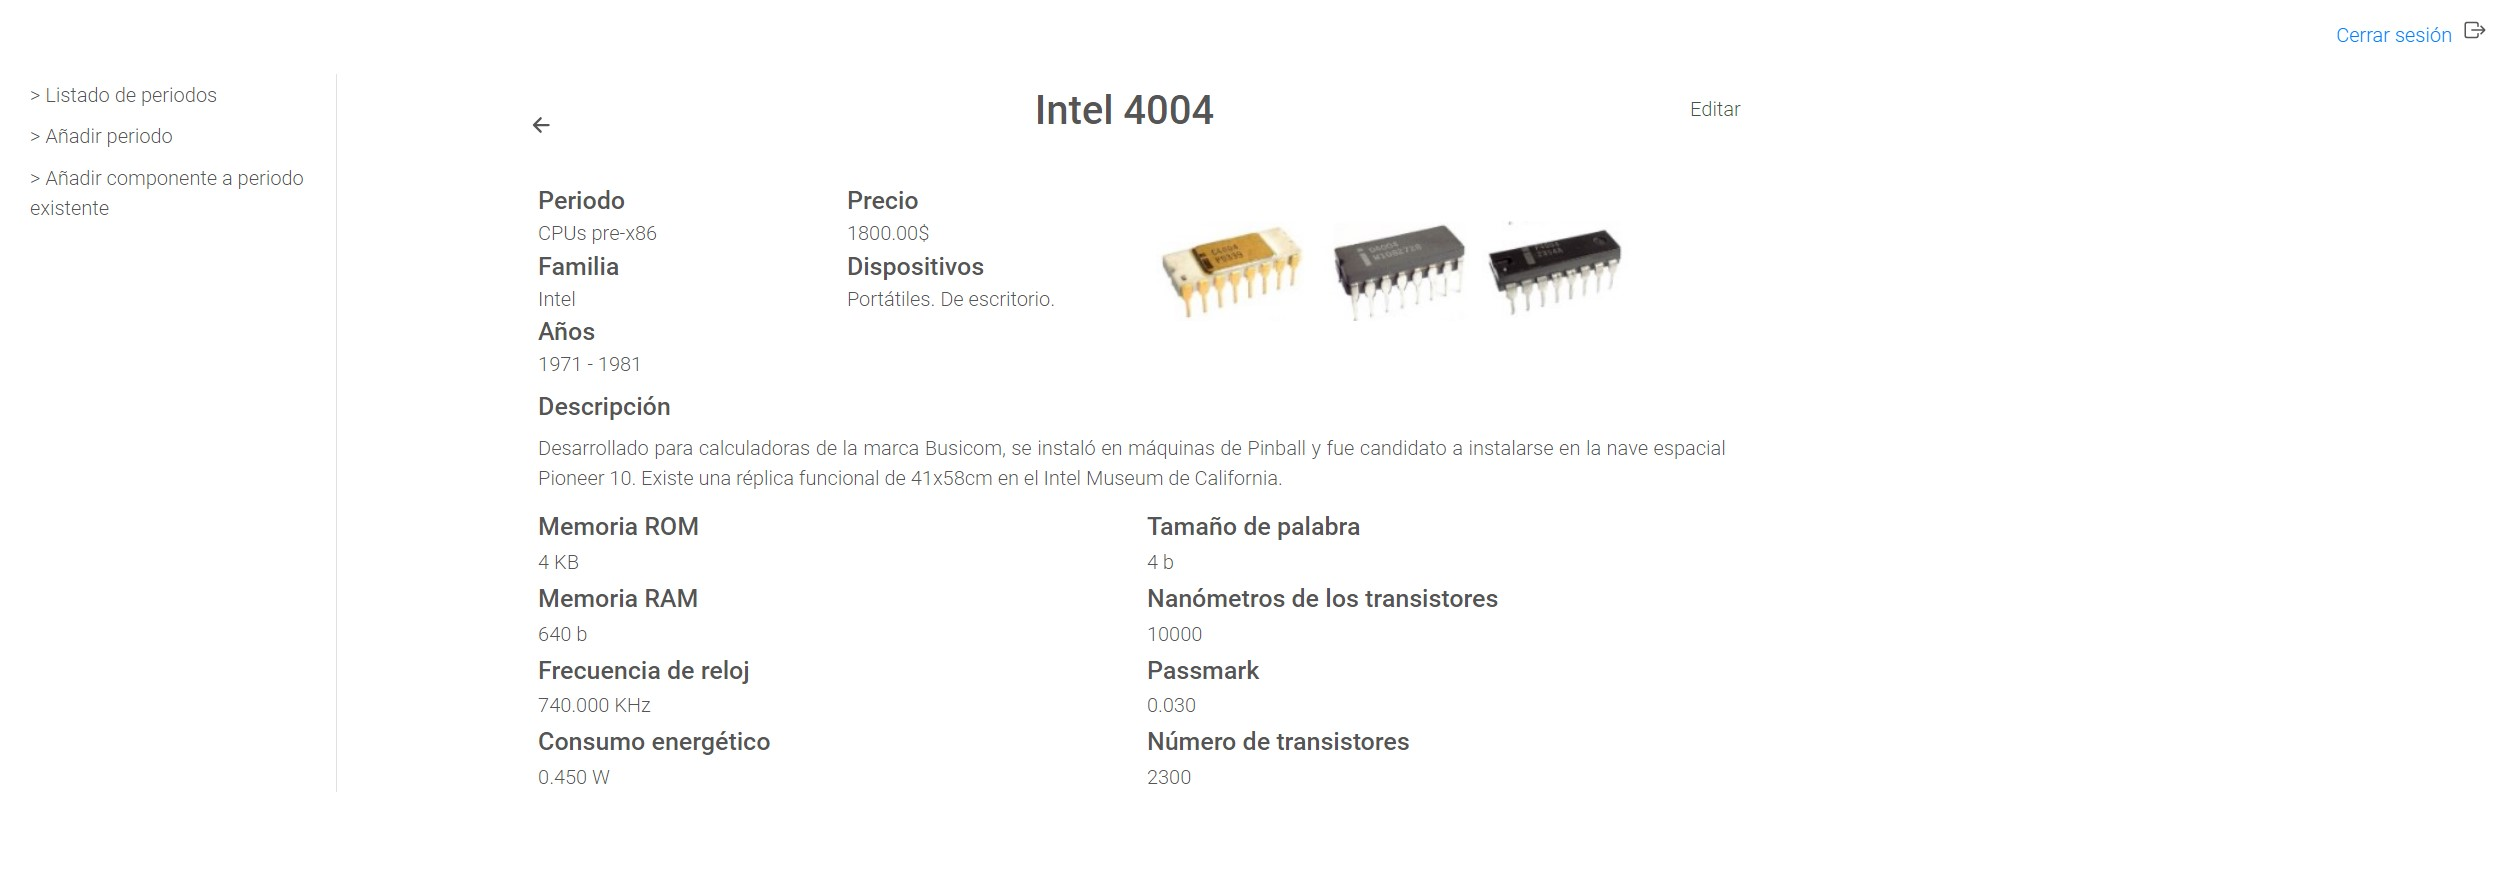
\includegraphics[scale=0.35]{compIUDef}
\caption{Manual de usuario: Detalles de un componente (administración)}
\end{figure}
En el formulario de añadir un periodo hay cuatro entradas de texto para nombre, detalles, curiosidades y eventos del periodo. Todos ellos deben rellenarse obligatoriamente para poder guardar el periodo. Si se pulsa el botón \textit{Cancelar}, el formulario se vaciará de nuevo. Al pulsar \textit{Guardar y continuar} con el formulario completo, se añadirá el periodo a la base de datos del sistema y nos redigirá al formulario para añadir componentes. En cambio, si el formulario no es válido se mostrará un error y no se añadirá.
\begin{figure}[H]
\centering
\includegraphics[scale=0.35]{añadirPeriodoIUDef}
\caption{Manual de usuario: Formulario para añadir un periodo}
\end{figure}
A la hora de editar un periodo, el formulario funcionará igual que al añadirlo, con la diferencia de que los valores iniciales serán los del periodo que se está editando.
\begin{figure}[H]
\centering
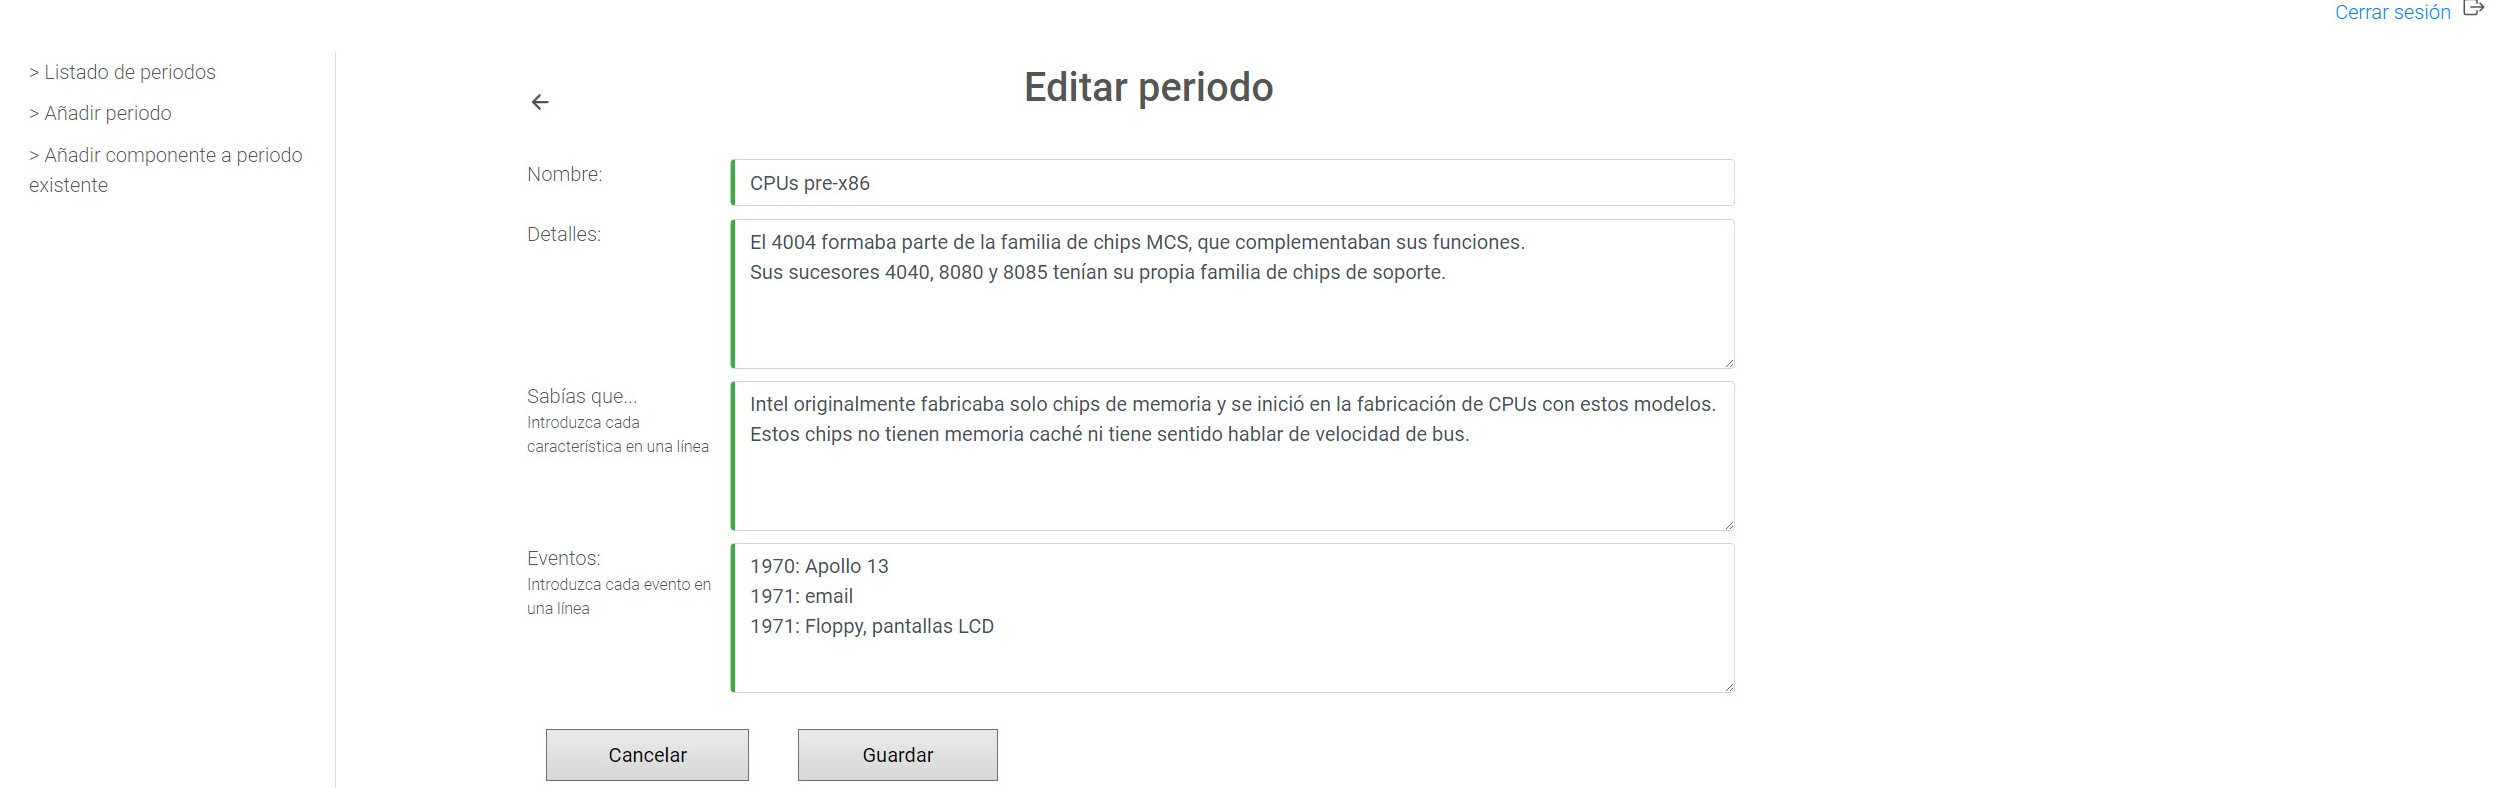
\includegraphics[scale=0.35]{editarPeriodoIUDef}
\caption{Manual de usuario: Formulario para editar un periodo}
\end{figure}
Los formularios para añadir y editar componentes funcionan de la misma forma que los de añadir y editar periodos, pero en este caso, hay campos que no son obligatorios, como la subida de imágenes y el sistema famoso. Además, al añadir o editar componentes se puede seleccionar su tipo: CPU o componente genérico. Al seleccionar CPU se muestran los campos de memoria ROM, memoria RAM, frecuencia de reloj, consumo energético, tamaño de palabra, nanómetros de transistores, passmark y número de transistores.
\begin{figure}[H]
\centering
\includegraphics[scale=0.35]{añadirCompIUDef}
\caption{Manual de usuario: Formulario para añadir un componente}
\end{figure}
\begin{figure}[H]
\centering
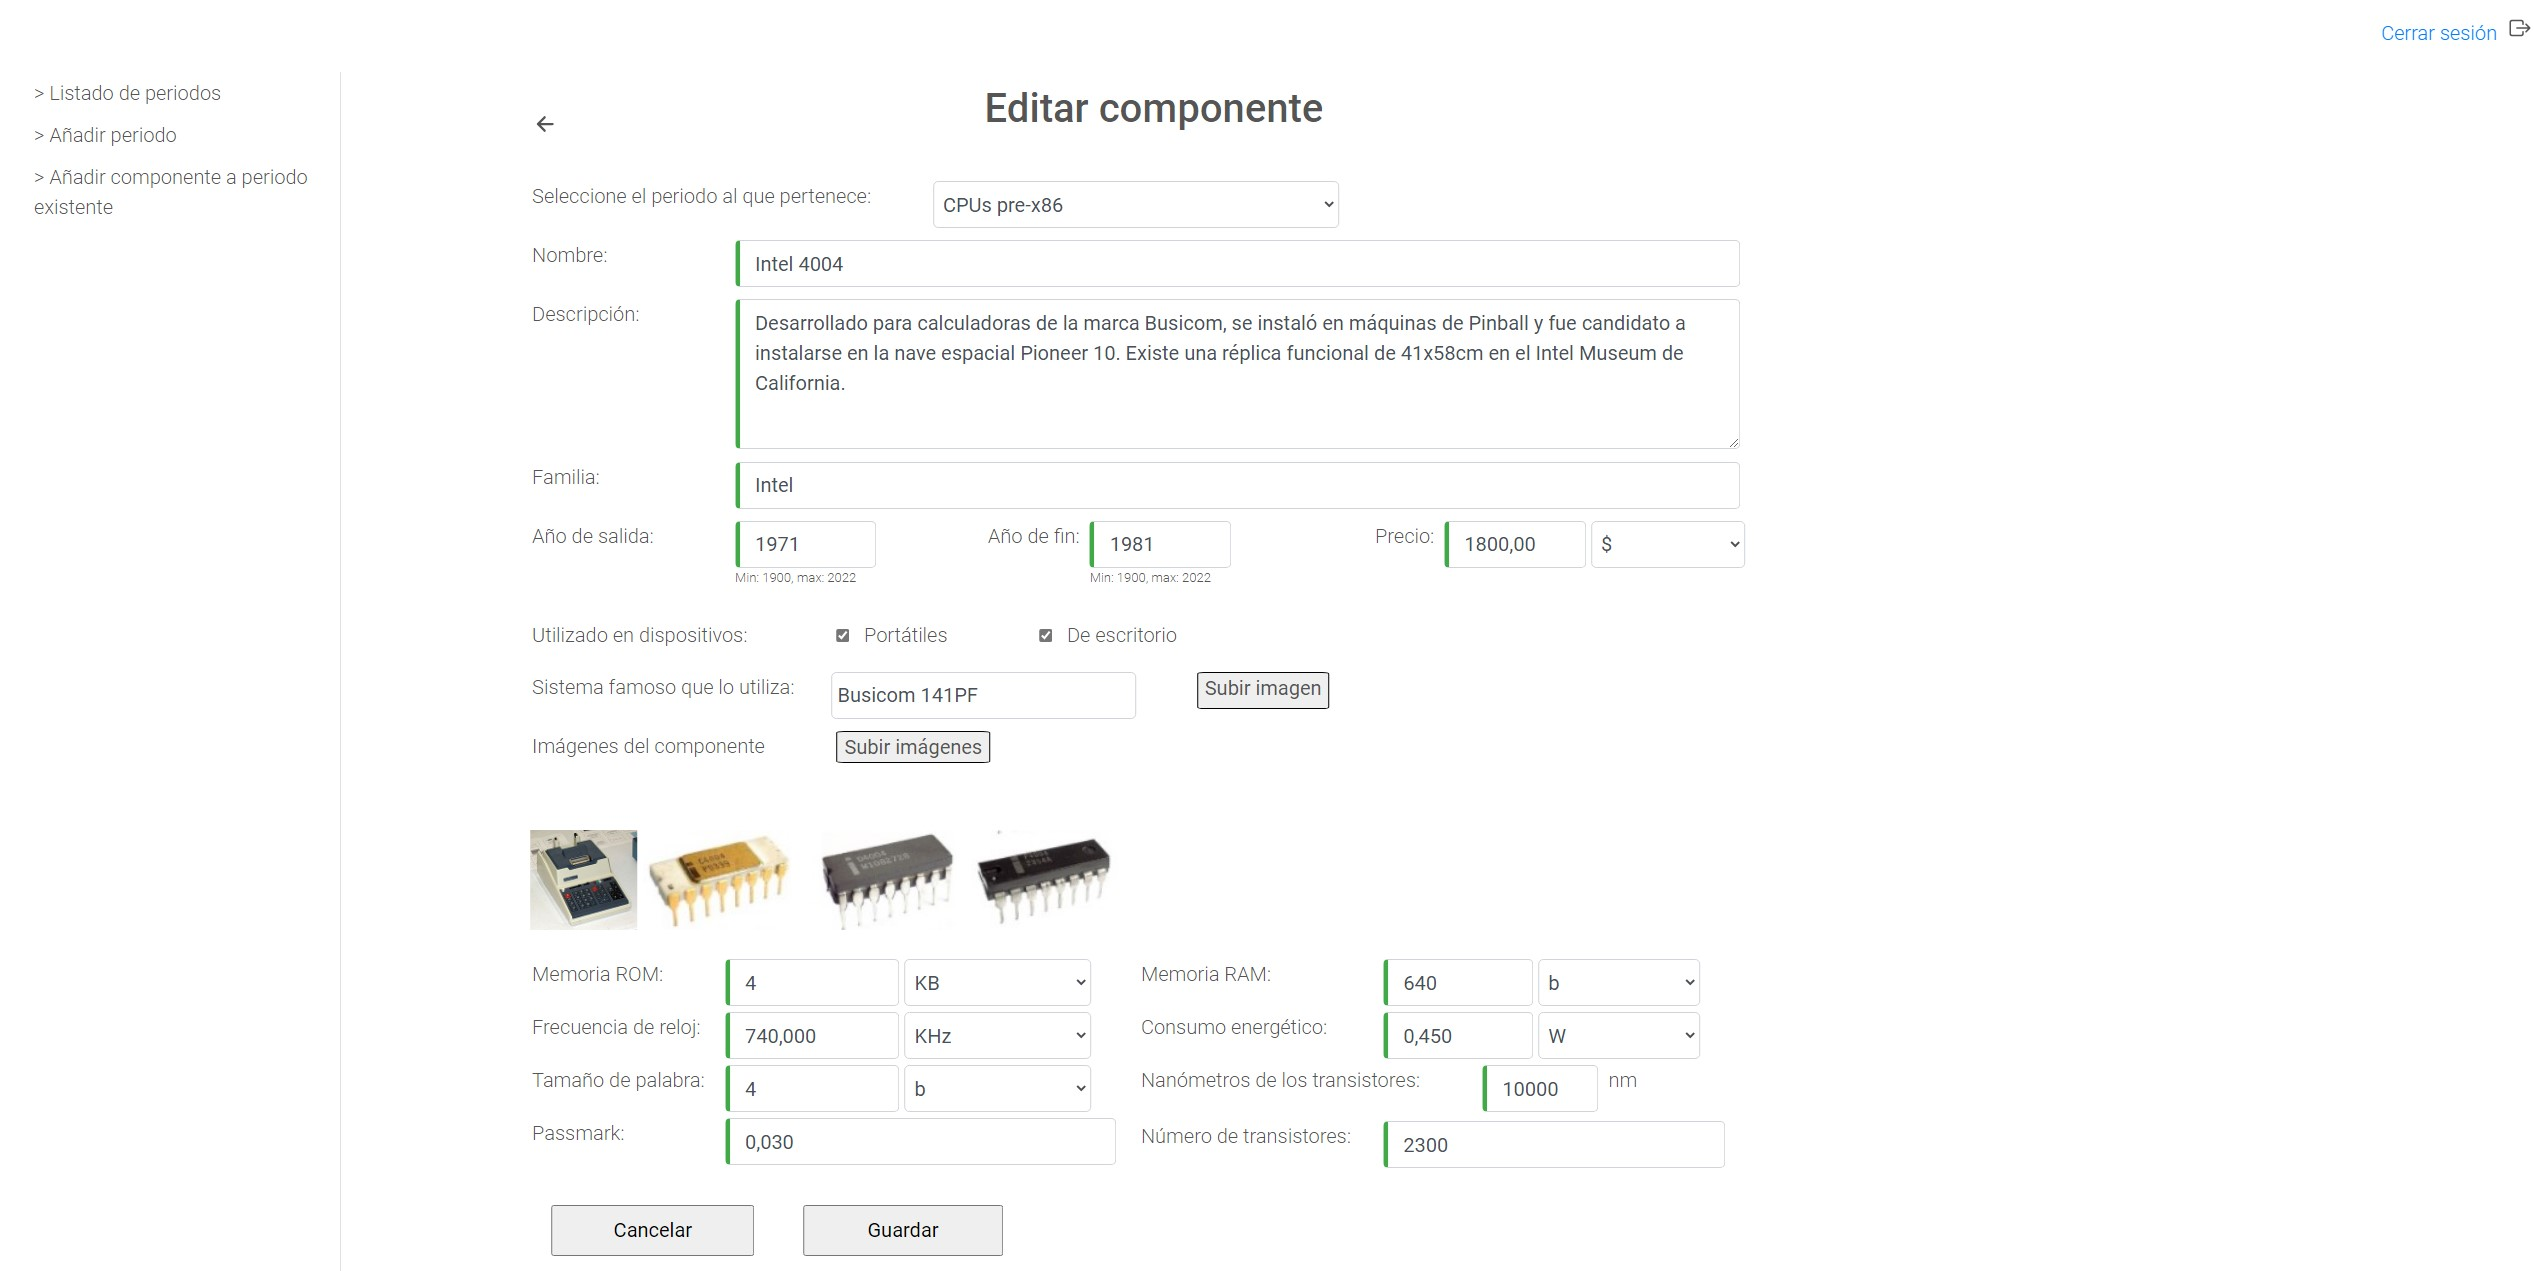
\includegraphics[scale=0.35]{editarCompIUDef}
\caption{Manual de usuario: Formulario para editar un componente}
\end{figure}


\subsection{Manual del Programador}
En este manual se explicará cómo ampliar la aplicación añadiendo nuevos tipos de componentes además de CPUs. Primero habría que crear una nueva clase para cada tipo que se desee añadir. Cada una de estas clases implementarán la interfaz \textit{MyComponent} y heredarán de \textit{GenericComp}. También habría que actualizar la enumeración \textit{CompTypes}. Estos tres elementos mencionados se encuentran en el archivo \textit{comp.ts}, que forma parte tanto del proyecto del museo (museo-eii) como de la administración (museo-eii-admin). Una vez realizado esto, común a ambos proyectos, se explicará qué debe añadirse a cada uno de ellos en específico, así como a la base de datos.

\subsubsection{Museo}
En el proyecto del museo (museo-eii) deberá generarse un componente de Angular para cada tipo añadido, se llamará \textit{`new type`DetailsComponent} y será hijo de \textit{CompDetailsComponent}, del que recibirá como input el atributo \textit{comp}. Este solo se mostrará cuando \textit{comp} sea una instancia del tipo correspondiente a `new type`. En \textit{`new type`-details.component.html} se listarán las características de \textit{comp}.\par
Además, en el método \textit{getComp} de \textit{CompDetailsComponent} habrá que añadir las comprobaciones necesarias para mostrar los nuevos tipos definidos.

\subsubsection{Administración del museo}
En el proyecto de la administración (museo-eii-admin) habrá que generar dos componentes de Angular nuevos por cada tipo añadido: 
\begin{itemize}
\item \textit{`new type`FormComponent}, hijo de \textit{AddCompComponent} y de \textit{EditCompComponent}. De ambos recibe como input el atributo \textit{model}. En \textit{`new type`-form.component.html} se incluirán los campos del formulario que se correspondan con las características del tipo creado. Se mostrará cuando \textit{model} sea una instancia del tipo correspondiente a `new type`. \par
En el método \textit{createModel} de \textit{AddCompComponent} habrá que añadir la opción de crear un objeto de este nuevo tipo, y también se añadirán las comprobaciones necesarias en los métodos \textit{isValid} y \textit{cloneComp} de \textit{AddCompComponent} y \textit{EditCompComponent}.
\item \textit{`new type`DetailsComponent}, hijo de \textit{MyComponentComponent}, del que recibe como input el atributo \textit{c}. En este caso, se hará exactamente lo mismo que lo mencionado anteriormente al añadir \textit{`new type`DetailsComponent} en el proyecto del museo, ya que ambos componentes son para mostrar las características de cada tipo.
\end{itemize}

\subsubsection{Base de datos}
En la base de datos habría que crear una tabla por cada nuevo tipo de componente, con los campos necesarios para este que no estén ya incluidos en la tabla \textit{components}. La clave primaria de esta tabla sería también una clave foránea, el identificador del componente en la tabla \textit{components}. Una vez creadas las tablas correspondientes, habría que modificar las comprobaciones y consultas realizadas en los archivos \textit{getComp.php, updateComp.php} y \textit{postComp.php} para incluir los nuevos tipos creados.


%\newpage
%\section{CSI 8: CONSTRUCCIÓN DE LOS COMPONENTES Y PROCEDIMIENTOS DE MIGRACIÓN Y CARGA INICIAL DE DATOS}



\newpage
\chapter{IMPLANTACIÓN Y ACEPTACIÓN DEL SISTEMA}
	\vspace{2cm}	
	\begin{center}
	{\Large \textbf{FASE DE DESARROLLO} \par}
	\end{center}
	\vspace{5cm}
	
	\begin{center}
	\Huge \textbf{IAS}\par
	\end{center}

\newpage

\section{IAS 1: ESTABLECIMIENTO DEL PLAN DE IMPLANTACIÓN}


\newpage
\section{IAS 4: CARGA DE DATOS AL ENTORNO DE OPERACIÓN}


%\newpage
%\section{IAS 5: PRUEBAS DE IMPLANTACIÓN DEL SISTEMA}


\newpage
\section{IAS 7: PREPARACIÓN DEL MANTENIMIENTO DEL SISTEMA}


%\newpage
%\section{IAS 8: ESTABLECIMIENTO DEL ACUERDO DE NIVEL DE SERVICIO}
%
%
%\newpage
%\section{IAS 9--10: PRESENTACIÓN Y APROBACIÓN DEL SISTEMA Y PASO A PRODUCCIÓN}
%

\newpage
\chapter{APÉNDICES}
\newpage

\section{PROBLEMAS ENCONTRADOS DURANTE EL DESARROLLO}

\newpage
\section{CONCLUSIONES}

\newpage
\section{AMPLIACIONES} 


%\newpage
%\section{REFERENCIAS BIBLIOGRÁFICAS}
\nocite{*} %El comando bibliography enseña solo las referencias que se hayan usado en el texto. Este comando permite "no citar" todas y así que aparezcan.
\bibliographystyle{ieeetr} 
\bibliography{references}

\newpage
\chapter{ANEXOS}
%\addcontentsline{toc}{chapter}{ANEXOS}
\newpage
%\phantomsection
\section{PLAN DE GESTIÓN DE RIESGOS}\label{sec:plan-riesgos}
%\addcontentsline{toc}{section}{PLAN DE GESTIÓN DE RIESGOS}
La gestión de los riesgos consiste en la identificación de los riesgos y la planificación para minimizar su efecto en el proyecto. Siguiendo la metodología del PMBOK \cite{PMBOK}, se define una gestión compuesta por los siguientes pasos:
\begin{itemize}
\item Planificar la Gestión de Riesgos.
\item Identificar los riesgos.
\item Realizar el análisis cualitativo de riesgos.
\item Realizar el análisis cuantitativo de riesgos.
\item Planificar la respuesta a los riesgos.
\item Monitorizar y controlar los riesgos.
\end{itemize}
A continuación se describirán los conceptos necesarios para planificar la gestión de riesgos, ya que los siguientes pasos se habrán realizado en la sección \ref{sec:riesgos}
\paragraph*{Categorías de riesgos}
Se categorizan los riesgos según la siguiente estructura de desglose:
\begin{figure}[H]
\centering
\centerline{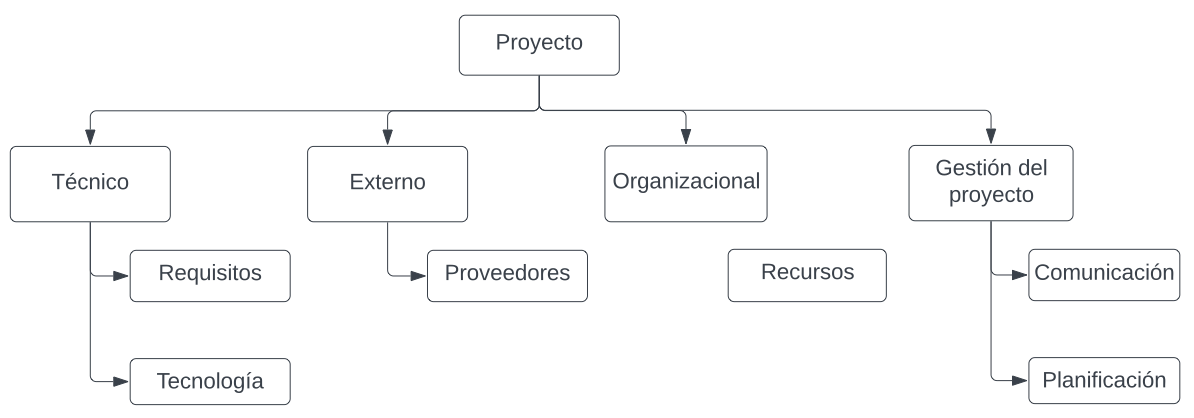
\includegraphics[scale=1.2]{rbs}}
\caption{Risk Breakdown Structure}
\end{figure}

\paragraph*{Probabilidad e impacto}
Se deben priorizar los riesgos de un proyecto en función de su probabilidad de ocurrencia e impacto. A continuación se muestra la definición de las probabilidades y las escalas de impacto para riesgos negativos.
\begin{figure}[H]
\centering
\centerline{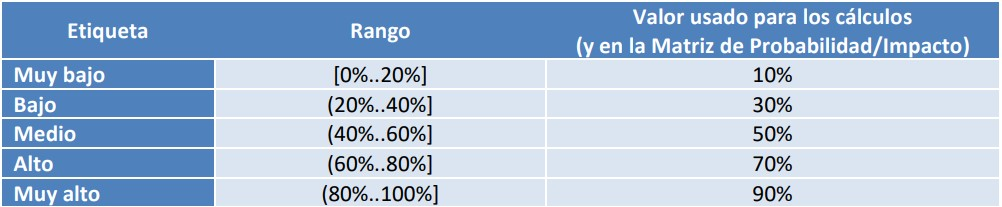
\includegraphics[scale=0.5]{def-probabilidades}}
\caption{Tabla de definición de probabilidades}
\end{figure}
\begin{figure}[H]
\centering
\centerline{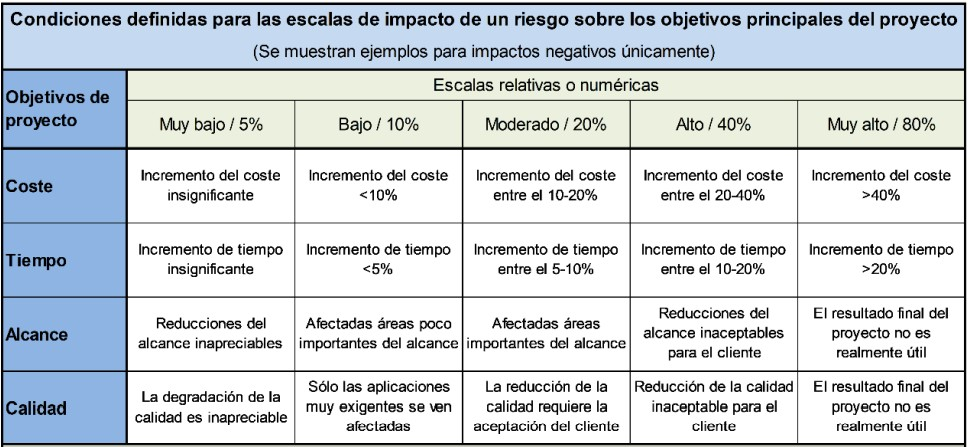
\includegraphics[scale=0.6]{escalas-impacto}}
\caption{Escalas de impacto sobre los objetivos del proyecto}
\end{figure}

\paragraph*{Matriz de probabilidad e impacto}
Esta matriz define los valores usados para priorizar los riesgos.
\begin{figure}[H]
\centering
\centerline{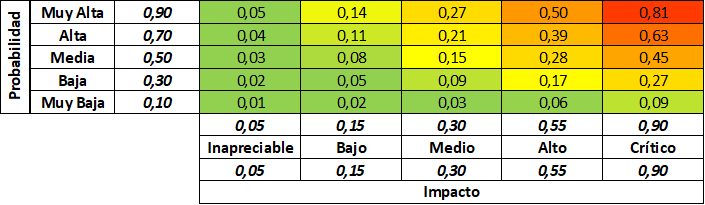
\includegraphics[scale=0.8]{matriz-prob}}
\caption{Matriz de Probabilidad e Impacto}
\end{figure}

\paragraph*{Estrategias de riesgo}
Para afrontar riesgos negativos se definen cuatro estrategias:
\begin{itemize}
\item Eliminar el riesgo.
\item Mitigar el riesgo.
\item Asumir el riesgo.
\item Transferir el riesgo.
\end{itemize}
Hay otras cuatro para riesgos positivos u oportunidades:
\begin{itemize}
\item Aprovechamiento.
\item Mejora.
\item Compartición.
\item Aceptación.
\end{itemize}


\newpage
\section{CONTENIDO ENTREGADO EN LOS ANEXOS}\label{sec:contenido_anexos}
%\addcontentsline{toc}{section}{CONTENIDO ENTREGADO EN LOS ANEXOS}

\subsection{Contenidos} 


Además de este documento, se hace entrega de una carpeta comprimida ``Entregables.zip'' en la que ahora se describirán sus contenidos. Se estructurará también la organización del código fuente.
\begin{itemize}
	\item \textbf{WBS.mpp} \(\rightarrow\) Archivo de Microsoft Project que contiene la planificación inicial del proyecto.
	\item \textbf{Presupuesto\_inicial.xlsx} \(\rightarrow\) Archivo Microsoft Excel que contiene los cálculos del presupuesto inicial del proyecto.
	\item \textbf{Presupuesto\_final.xlsx} \(\rightarrow\) Archivo Microsoft Excel que contiene los cálculos del presupuesto final del proyecto.
	\item \textbf{Informe\_Riesgos.xlsx} \(\rightarrow\) Archivo Microsoft Excel con el cálculo de probabilidad e impacto de los riesgos del proyecto.
	\item \textbf{Documentación\_Compodoc} \(\rightarrow\) Carpeta que contiene la documentación de los proyectos (museo y administración) generada con Compodoc. Abriendo el archivo \textit{index.html} de cada una de ellas se muestra la documentación correspondiente.
	\begin{itemize}
		\item \textbf{Documentación\_Museo} \(\rightarrow\) Contiene la documentación del proyecto del museo (museo-eii).
		\item \textbf{Documentación\_Admin} \(\rightarrow\) Contiene la documentación del proyecto de la administración del museo (museo-eii-admin).
	\end{itemize}
 	Cada una de estas carpetas contiene los archivos HTML con la documentación generada. Abriendo el archivo \textit{index.html} de cada una se puede ver la documentación al completo de su respectivo proyecto.
	\item \textbf{Diagramas} \(\rightarrow\) Carpeta que contiene todos los diagramas utilizados en este documento.
	\begin{itemize}
		\item \textit{Diagrama\_arquitectura\_tecnologica.png}
		\item \textit{Diagrama\_casos\_uso\_museo.png}
		\item \textit{Diagrama\_casos\_uso\_admin.png}
		\item \textit{Diagrama\_clases\_museo-Analisis.png}
		\item \textit{Diagrama\_clases\_admin-Analisis.png}
		\item \textit{Diagrama\_navegabilidad\_museo.png}
		\item \textit{Diagrama\_navegabilidad\_admin.png}
		\item \textit{Diagrama\_clases\_museo-Diseño.png}
		\item \textit{Diagrama\_clases\_admin-Diseño.png}
		\item \textit{Diagrama\_paquetes.png}
		%\item \textit{Diagrama\_componentes.png}
		\item \textit{Diagrama\_despliegue.png}
		\item \textit{Diagrama\_E-R.png}
		\item \textit{PBS.png}
		\item \textit{RBS.png}
	\end{itemize}
	\item \textbf{Codigo.zip} \(\rightarrow\) Carpeta comprimida con todo el código fuente. Está dividida a su vez en tres carpetas:
	\begin{itemize}
		\item \textbf{museo-eii} \(\rightarrow\) Contiene el proyecto de la aplicación del museo.
		\item \textbf{museo-eii-admin} \(\rightarrow\) Contiene el proyecto de la administración del museo.
		\item \textbf{back-end} \(\rightarrow\) Contiene los archivos PHP necesarios para conectarse con la base de datos del sistema, así como el script de creación de la base de datos e inserción de los datos iniciales. También tiene una carpeta \textit{upload}, con las imágenes de los componentes insertados a través del script.
	\end{itemize}
	museo-eii y museo-eii-admin tienen la misma estructura en su contenido. Ambas carpetas contienen:
	\begin{itemize}
		\item Carpeta \textbf{dist}: contiene los archivos necesarios para la distribución del proyecto.
		\item Carpeta \textbf{src}: contiene el código fuente del proyecto.
		\item \textbf{src/assets}: contiene las imágenes utilizadas en la aplicación y los archivos de internacionalización.
		\item \textbf{src/app}: contiene las clases (carpeta classes), los servicios (carpeta services) y los componentes de la aplicación (cada uno de ellos con su propia carpeta). Cada uno de estos elementos es un archivo \textit{.ts} donde se encuentra la funcionalidad correspondiente, al que acompaña un archivo \textit{.spec.ts} con las pruebas unitarias. Además los componentes también tienen asociados un archivo HTML y otro CSS para su visualización.
	\end{itemize} 
\par Se incluye un archivo \textit{README.md} con las instrucciones para la ejecución de ambos proyectos.
\end{itemize}



%\newpage
%\nocite{*} %El comando bibliography enseña solo las referencias que se hayan usado en el texto. Este comando permite "no citar" todas y así que aparezcan.
%\bibliographystyle{ieeetr} 
%\bibliography{references}
\newpage





\end{document}
